%                                                                 aa.dem
% AA vers. 9.1, LaTeX class for Astronomy & Astrophysics
% demonstration file
%                                                       (c) EDP Sciences
%-----------------------------------------------------------------------
%
%\documentclass[referee]{aa} % for a referee version
%\documentclass[onecolumn]{aa} % for a paper on 1 column  
%\documentclass[longauth]{aa} % for the long lists of affiliations 
%\documentclass[letter]{aa} % for the letters 
%\documentclass[bibyear]{aa} % if the references are not structured 
%                              according to the author-year natbib style

%
\documentclass{aa}  
\renewcommand{\arraystretch}{1.4}
\graphicspath{ {./imgs/} }

%
\usepackage{graphicx}
\usepackage{lscape}
%%%%%%%%%%%%%%%%%%%%%%%%%%%%%%%%%%%%%%%%
\usepackage{txfonts}
%%%%%%%%%%%%%%%%%%%%%%%%%%%%%%%%%%%%%%%%
%\usepackage[options]{hyperref}
% To add links in your PDF file, use the package "hyperref"
% with options according to your LaTeX or PDFLaTeX drivers.
%
\begin{document} 


   \title{Chemistry Study on Hot Corino Serpen South CARMA-7}



   \author{Haotian Liu (under supervision of Dr. Adele L. Plunkett)}

   \institute{University of Virginia,
              \email{hl7gr@virginia.edu}}




% \abstract{}{}{}{}{} 
% 5 {} token are mandatory
 
  \abstract
  % context heading (optional)
  % {} leave it empty if necessary  
   {To study the interesting chemistry of a newly found hot corino CARMA-7 in Serpen South region}
  % aims heading (mandatory)
   {Chemical line identification and source motion analysis}
  % methods heading (mandatory)
   {CASA ADMIT + other spectral processing tools}
  % results heading (mandatory)
   {See line identification and conclusion}
  % conclusions heading (optional), leave it empty if necessary 
   {}

   \keywords{Hot corino, Astrochemistry, Scientific computing}

   \maketitle
%
%-------------------------------------------------------------------

\section{Introduction}

    This thesis contains spectral line analysis of 6 spectral windows of ALMA observation on source Serpen South CARMA-7.

%--------------------------------------------------------------------
\section{Observation}
   ALMA observation was conducted with 6 spectral windows.
\begin{table*}   
 \label{table:1}  
     \caption{Line identification results for spectral window 0}
 \tiny
    \centering    
    \begin{tabular}{l l l l l l l l l} 
    \hline    
    Molecule & Name &Transition & Frequency & $E_{u}$ & Intensity & Velocity & $v_{lsr}$ & Peak / rms\\ 
    \hline   
$(CH_{3})_{2}CO$ & Acetone & $33_{2,32}-32_{2,31}AE$ & $336.94769$ & $284.9779$ & $5.8645$ & $6.7346$ & $8.0$ & $8.2528$\\
$c-HCCCH$ & Cyclopropenylidene & $4_{4,1}-3_{1,2}$ & $336.94859$ & $32.2203$ & $7.7754$ & $8.5402$ & $8.0$ & $10.942$\\
$g'Ga-(CH_{2}OH)_{2}$ & Ethylene Glycol & $29_{17,12}v=0-29_{16,13}v=0$ & $336.95735$ & $355.5986$ & $22.9795$ & $7.6964$ & $8.0$ & $32.3382$\\
$(CH_{3})_{2}CO$ & Acetone & $33_{1,32}-32_{2,31}EE$ & $336.96839$ & $284.9042$ & $8.6102$ & $8.9506$ & $8.0$ & $12.1167$\\
$(CH_{3})_{2}CO$ & Acetone & $24_{12,13}-23_{11,12}EE$ & $336.97681$ & $230.3935$ & $2.1859$ & $6.0204$ & $8.0$ & $3.0761$\\
$(CH_{3})_{2}CO$ & Acetone & $33_{1,32}-32_{2,31}AA$ & $336.98907$ & $284.8304$ & $3.5648$ & $9.0125$ & $8.0$ & $5.0166$\\
$H_{2}NCH_{2}CN$ & Aminoacetonitrile & $37_{5,33}-36_{5,32}$ & $337.01833$ & $337.6508$ & $8.1389$ & $8.8251$ & $8.0$ & $11.4536$\\
$g-CH_{3}CH_{2}OH$ & gauche-Ethanol & $36_{5,32}-35_{6,29},vt=0-0$ & $337.02461$ & $643.1397$ & $8.0259$ & $13.0103$ & $8.0$ & $11.2946$\\
$c-H_{13}CCCH$ & Cyclopropenylidene & $21_{11,10}-21_{11,11}$ & $337.02915$ & $649.5308$ & $0.0$ & $0.0$ & $8.0$ & $0.0$\\
$CH_{2}CHCN$ & Vinyl Cyanide & $36_{2,35}-35_{2,34}$ & $337.03974$ & $309.7482$ & $6.3892$ & $7.3691$ & $8.0$ & $8.9912$\\
$C_{17}O$ & Carbon Monoxide & $J=3-2$ & $337.0611$ & $32.3538$ & $32.425$ & $0.5295$ & $8.0$ & $45.6304$\\
$g'Ga-(CH_{2}OH)_{2}$ & Ethylene Glycol & $33_{8,25}v=0-32_{8,24}v=1$ & $337.08211$ & $309.0677$ & $6.6297$ & $5.9492$ & $8.0$ & $9.3296$\\
$cis-CH_{2}OHCHO$ & Glycolaldehyde & $29_{13,17}-28_{13,16}$ & $337.09926$ & $344.463$ & $20.9463$ & $7.5278$ & $8.0$ & $29.4769$\\
$cis-CH_{2}OHCHO$ & Glycolaldehyde & $29_{13,16}-28_{13,15}$ & $337.09927$ & $344.463$ & $0.0$ & $0.0$ & $8.0$ & $0.0$\\
$g'Ga-(CH_{2}OH)_{2}$ & Ethylene Glycol & $69_{18,52}v=1-69_{17,53}v=1$ & $337.10336$ & $1346.196$ & $-0.0118$ & $8.1634$ & $8.0$ & $-2.8258$\\
$CH_{3}NH_{2}$ & Methylamine & $2_{2}E2-1-1_{1}E2-1,F=2-2$ & $337.11864$ & $22.2636$ & $0.0$ & $0.0$ & $8.0$ & $0.0$\\
$CH_{3}NH_{2}$ & Methylamine & $2_{2}E2-1-1_{1}E2-1,F=2-1$ & $337.11894$ & $22.2636$ & $8.052$ & $3.7404$ & $8.0$ & $11.3313$\\
$CH_{3}OHvt=_{0}$ & Methanol & $3_{3,0}-4_{2,2}$ & $337.13586$ & $61.6392$ & $36.2978$ & $7.6565$ & $8.0$ & $51.0804$\\
$cis-CH_{2}OHCHO$ & Glycolaldehyde & $15_{7,9}-14_{6,8}$ & $337.15086$ & $96.4924$ & $2.1438$ & $7.3493$ & $8.0$ & $3.0169$\\
$CH_{3}CHO$ & Acetaldehyde & $13_{1,12}-12_{-1,12}E$ & $337.15207$ & $88.4514$ & $0.0247$ & $6.2404$ & $8.0$ & $5.9389$\\
$g'Ga-(CH_{2}OH)_{2}$ & Ethylene Glycol & $26_{17,9}v=1-26_{16,10}v=1$ & $337.16832$ & $314.6439$ & $0.0147$ & $7.4294$ & $8.0$ & $3.5352$\\
$g'Ga-(CH_{2}OH)_{2}$ & Ethylene Glycol & $24_{17,7}v=0-24_{16,8}v=0$ & $337.17585$ & $289.264$ & $0.0$ & $0.0$ & $8.0$ & $0.0$\\

    \hline                  
    \end{tabular}
\end{table*}


   \begin{figure*}
    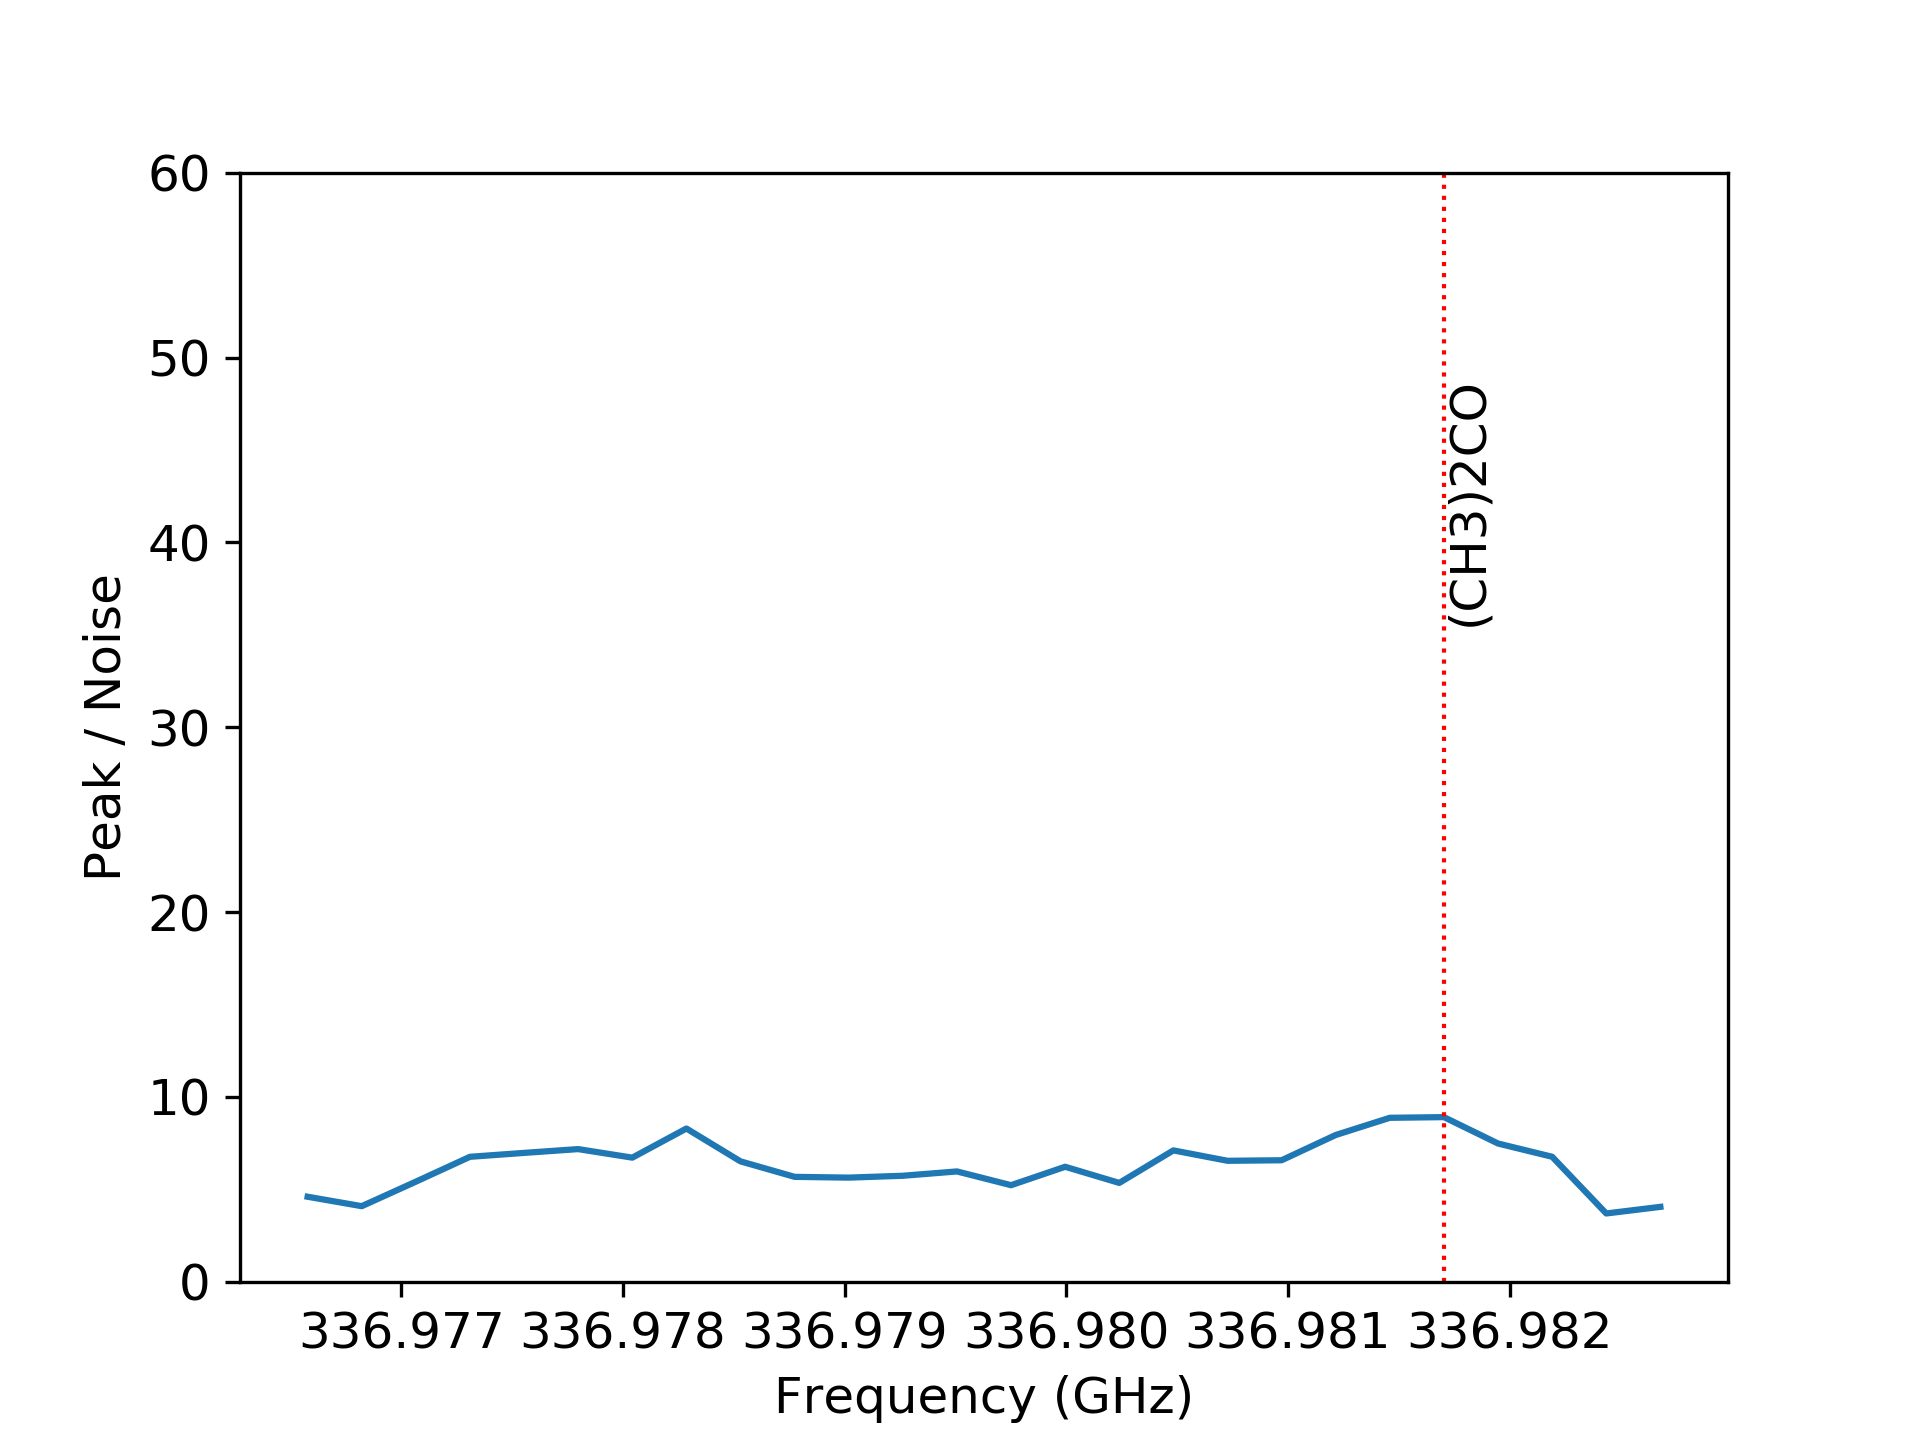
\includegraphics[width=0.33\textwidth]{spw0_(CH3)2CO}
    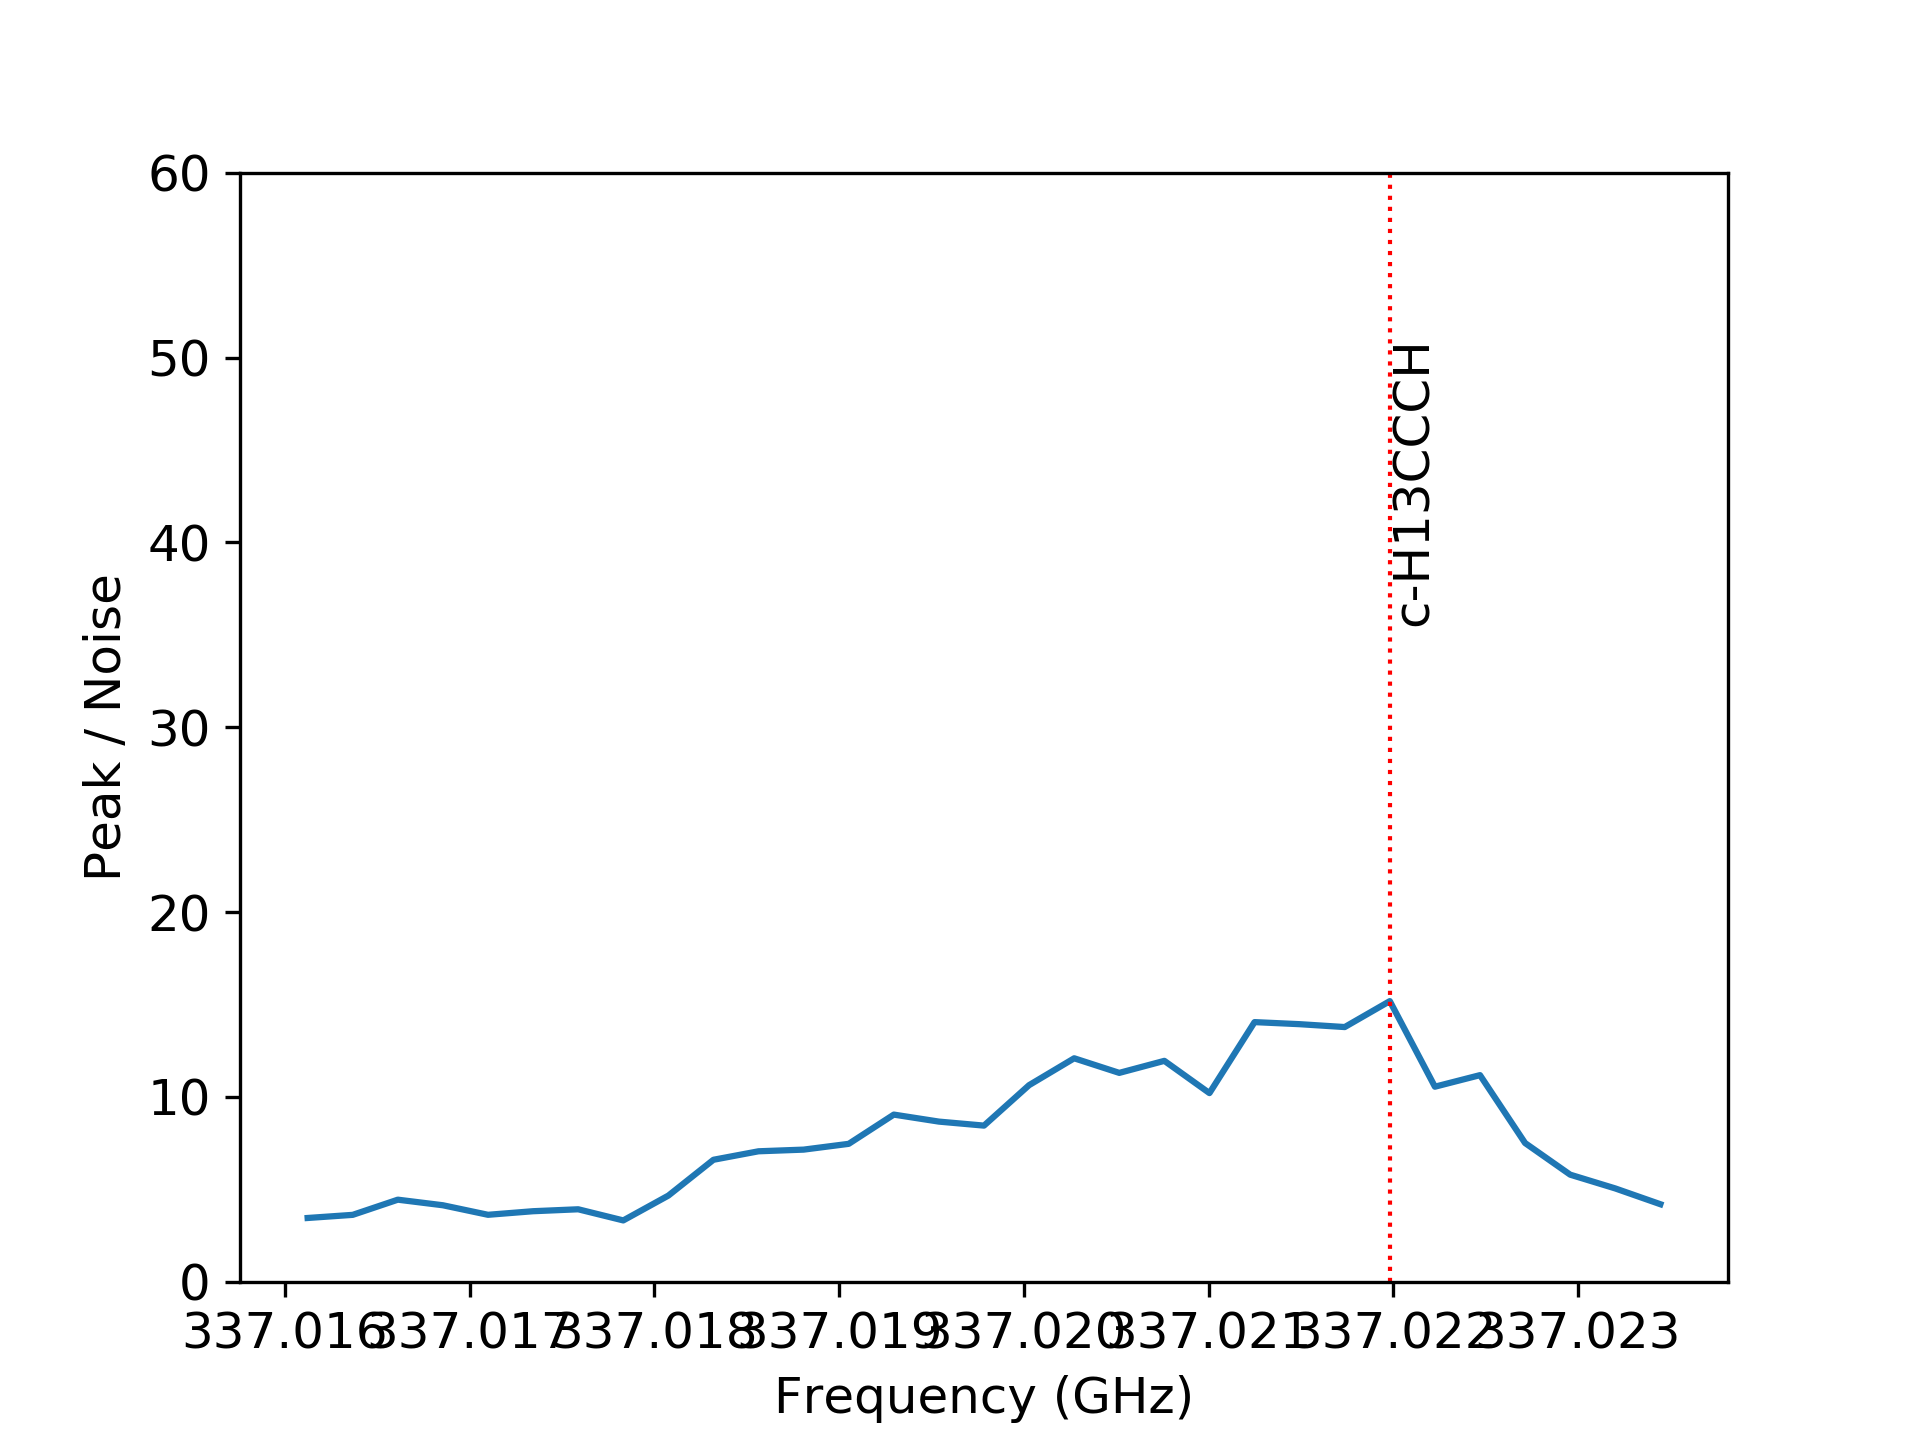
\includegraphics[width=0.33\textwidth]{spw0_c-H13CCCH}
    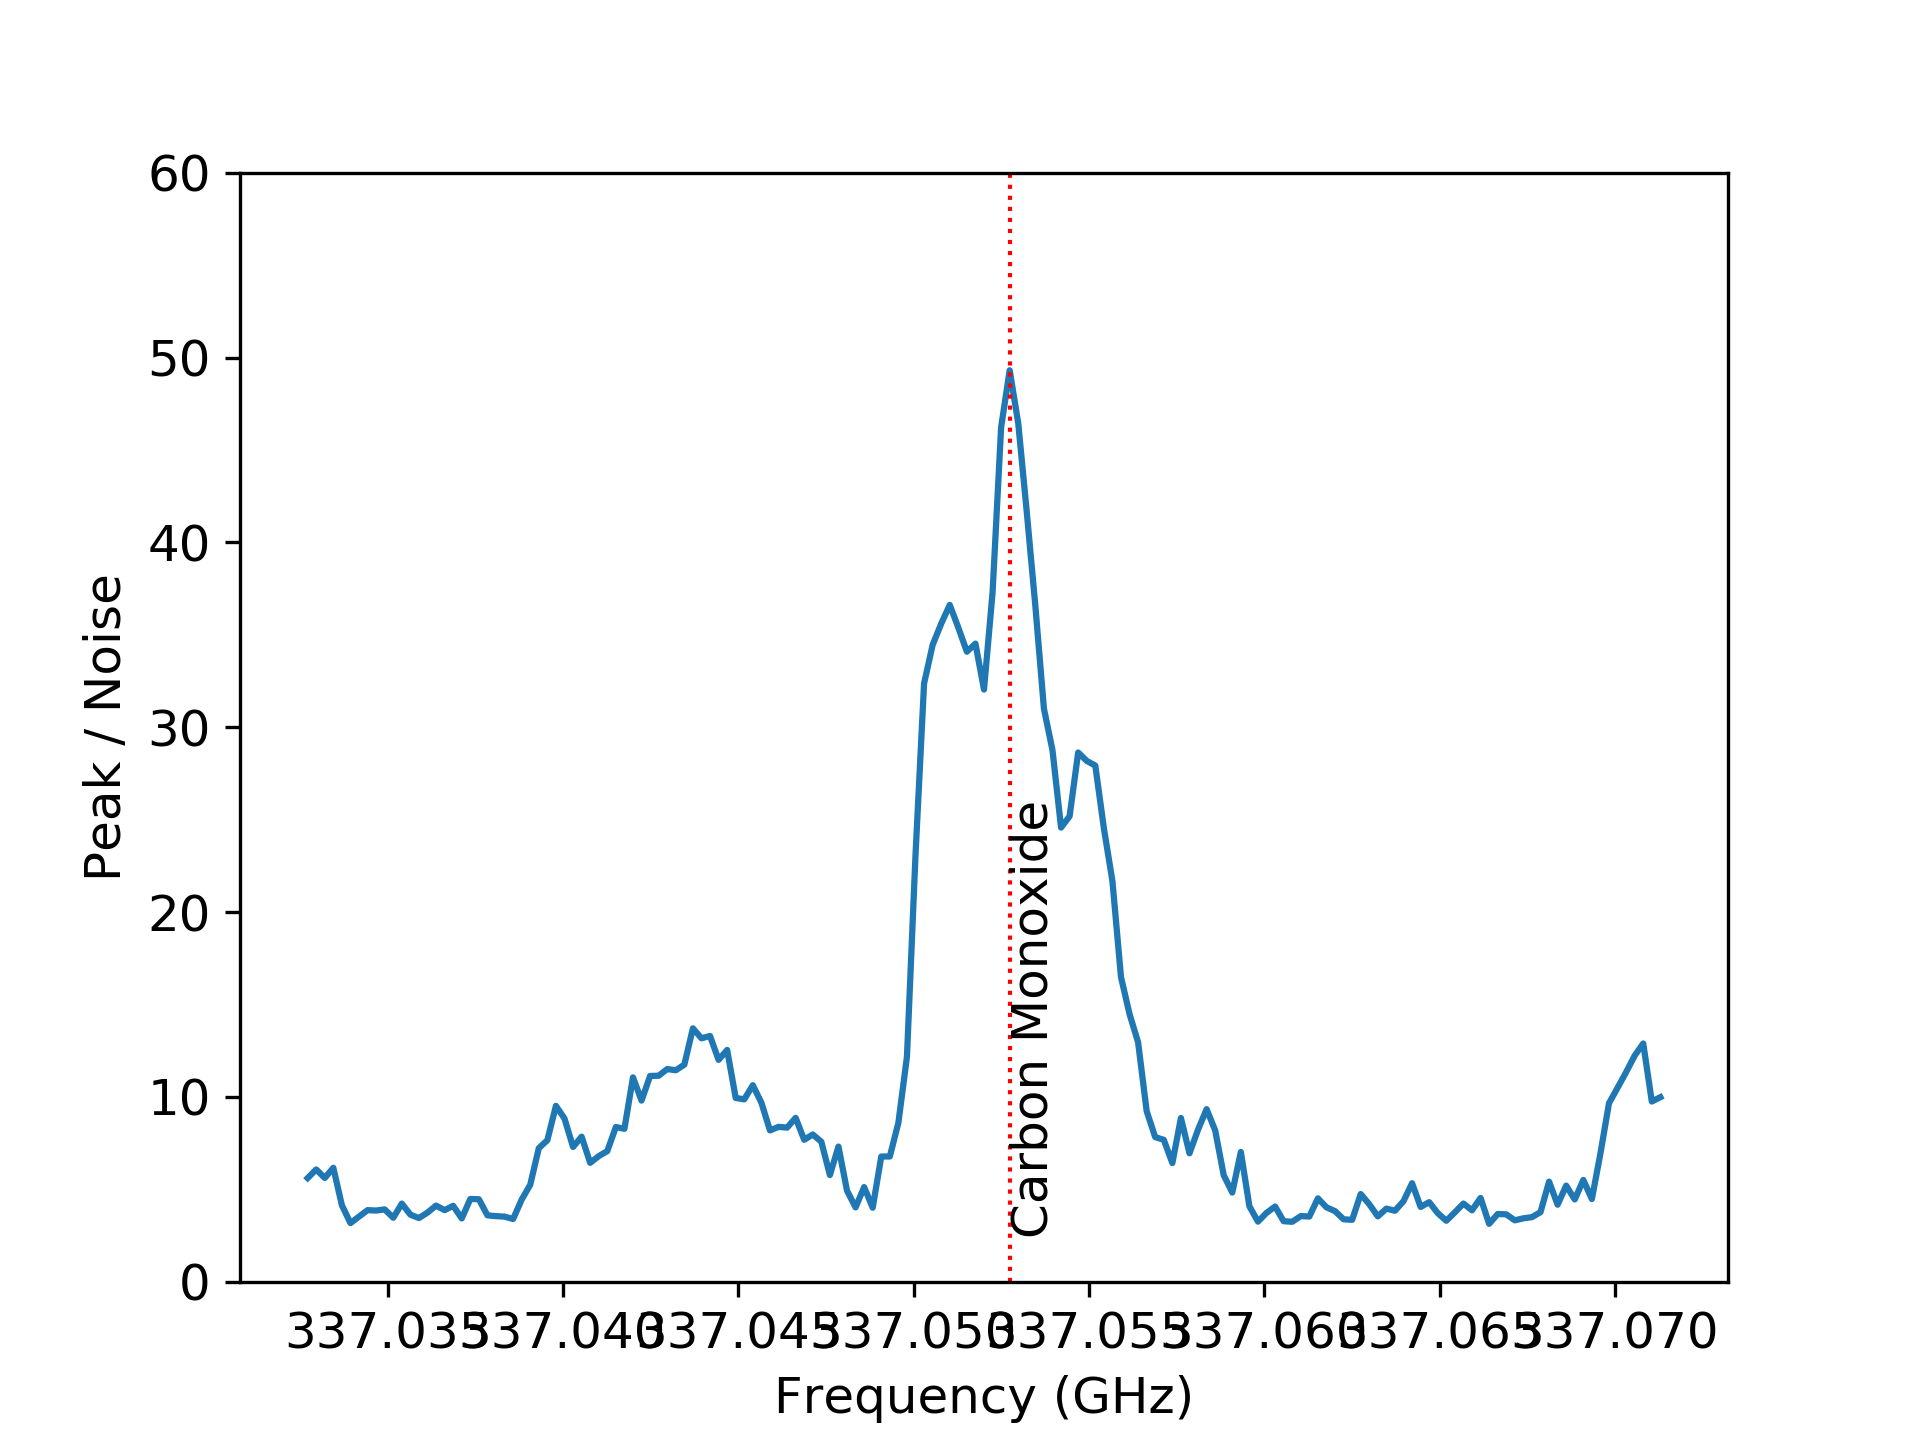
\includegraphics[width=0.33\textwidth]{spw0_C17O}
    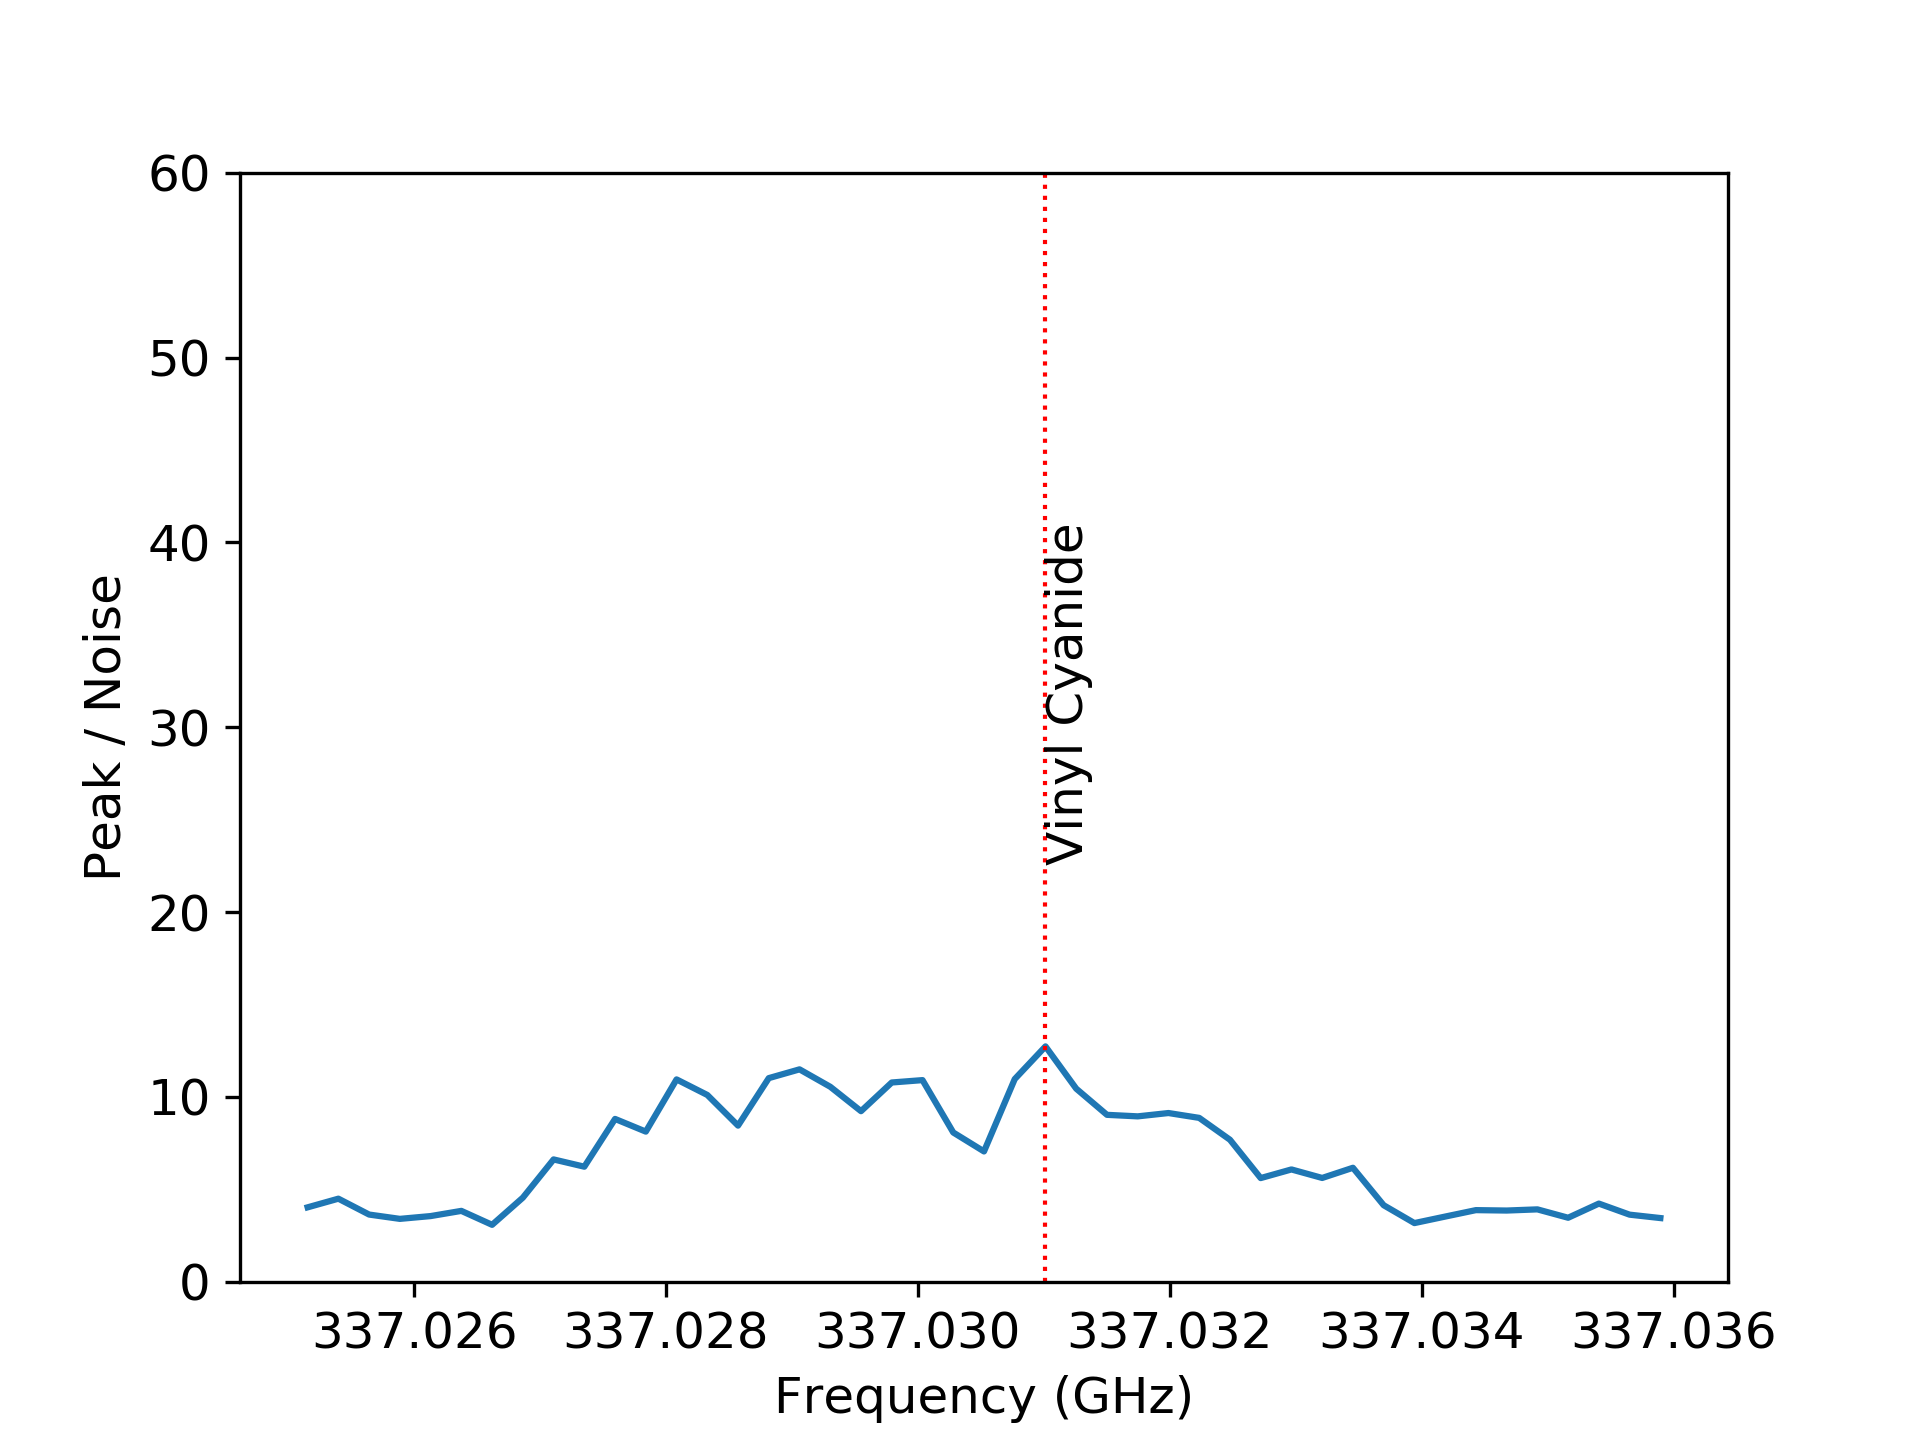
\includegraphics[width=0.33\textwidth]{spw0_CH2CHCN}
    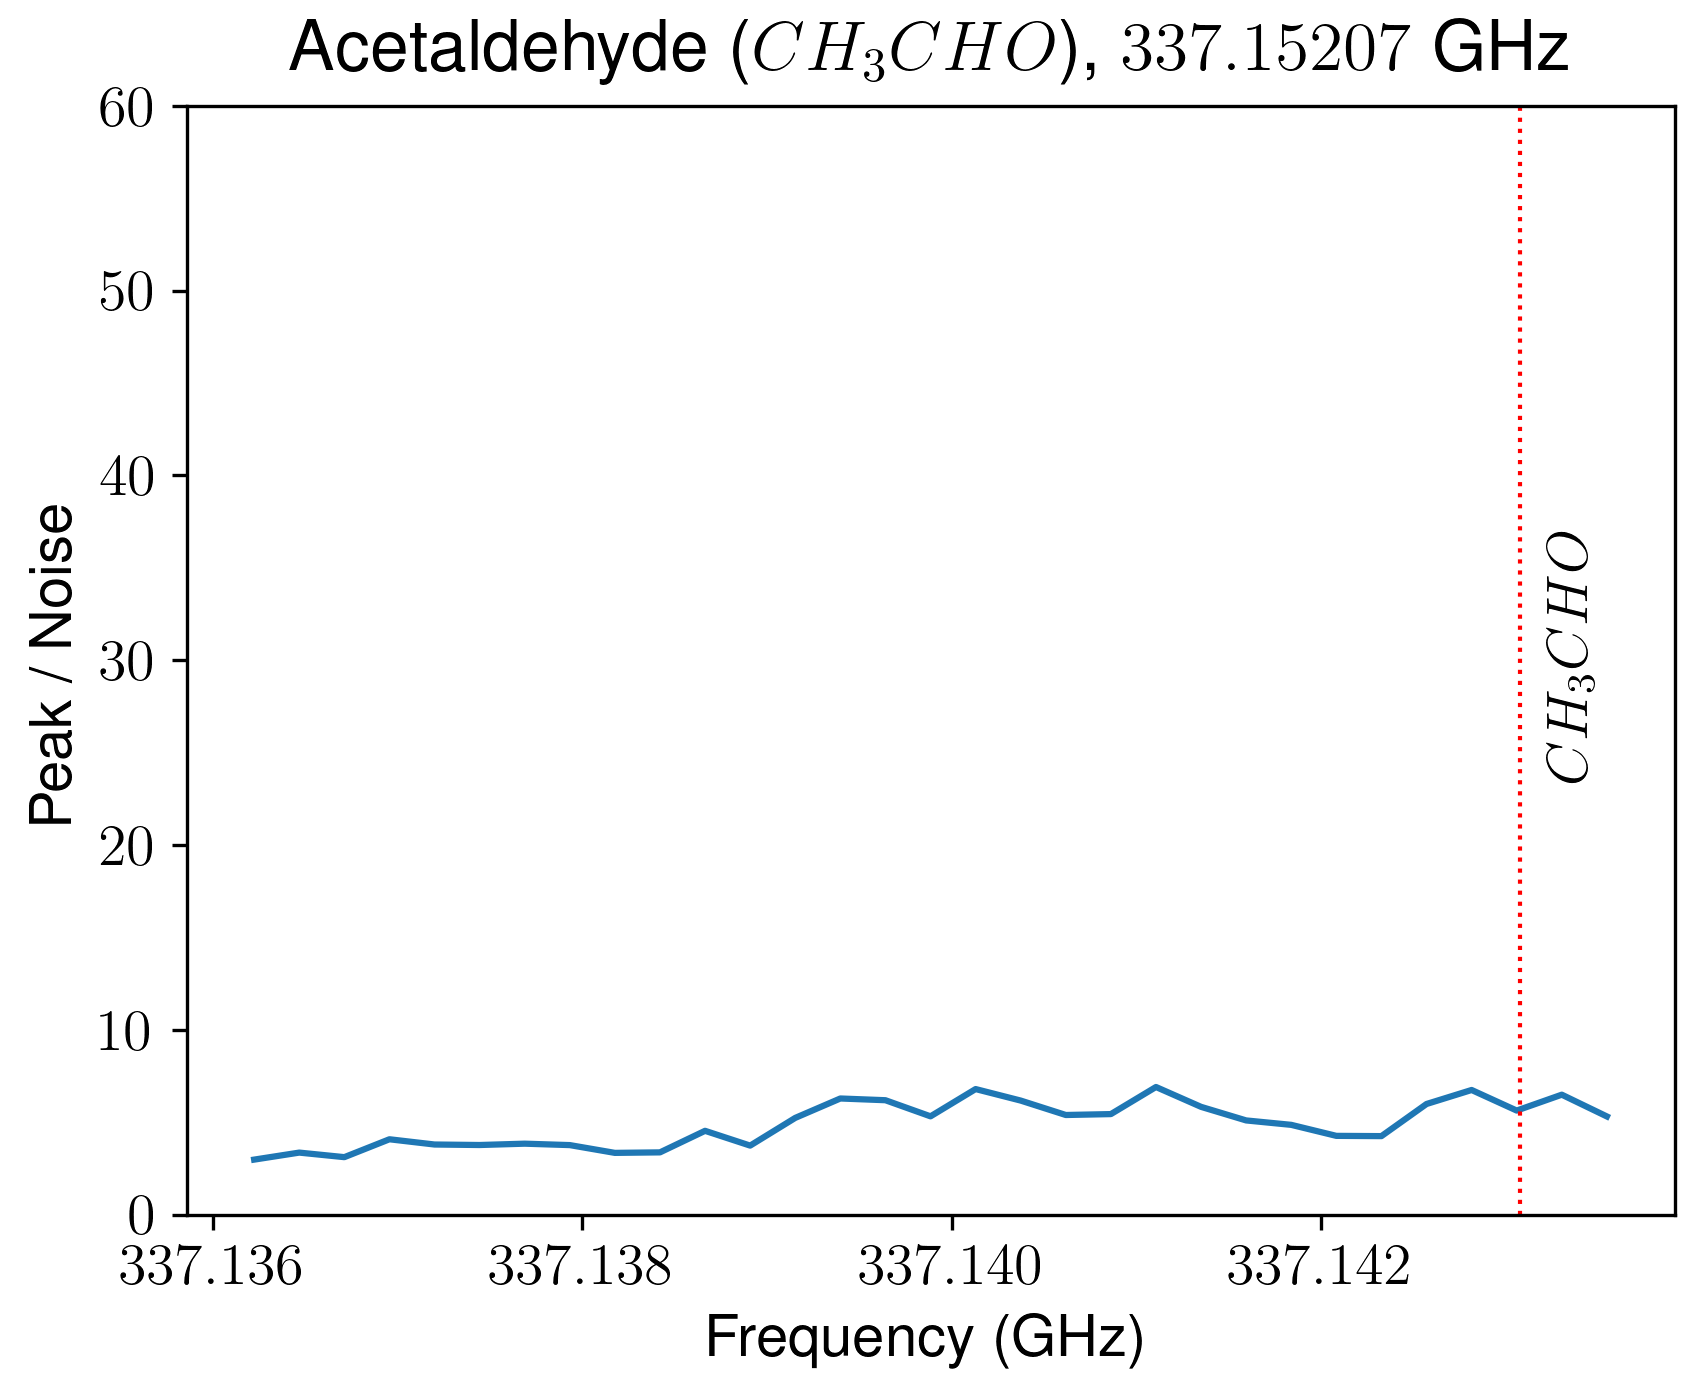
\includegraphics[width=0.33\textwidth]{spw0_CH3CHO}
    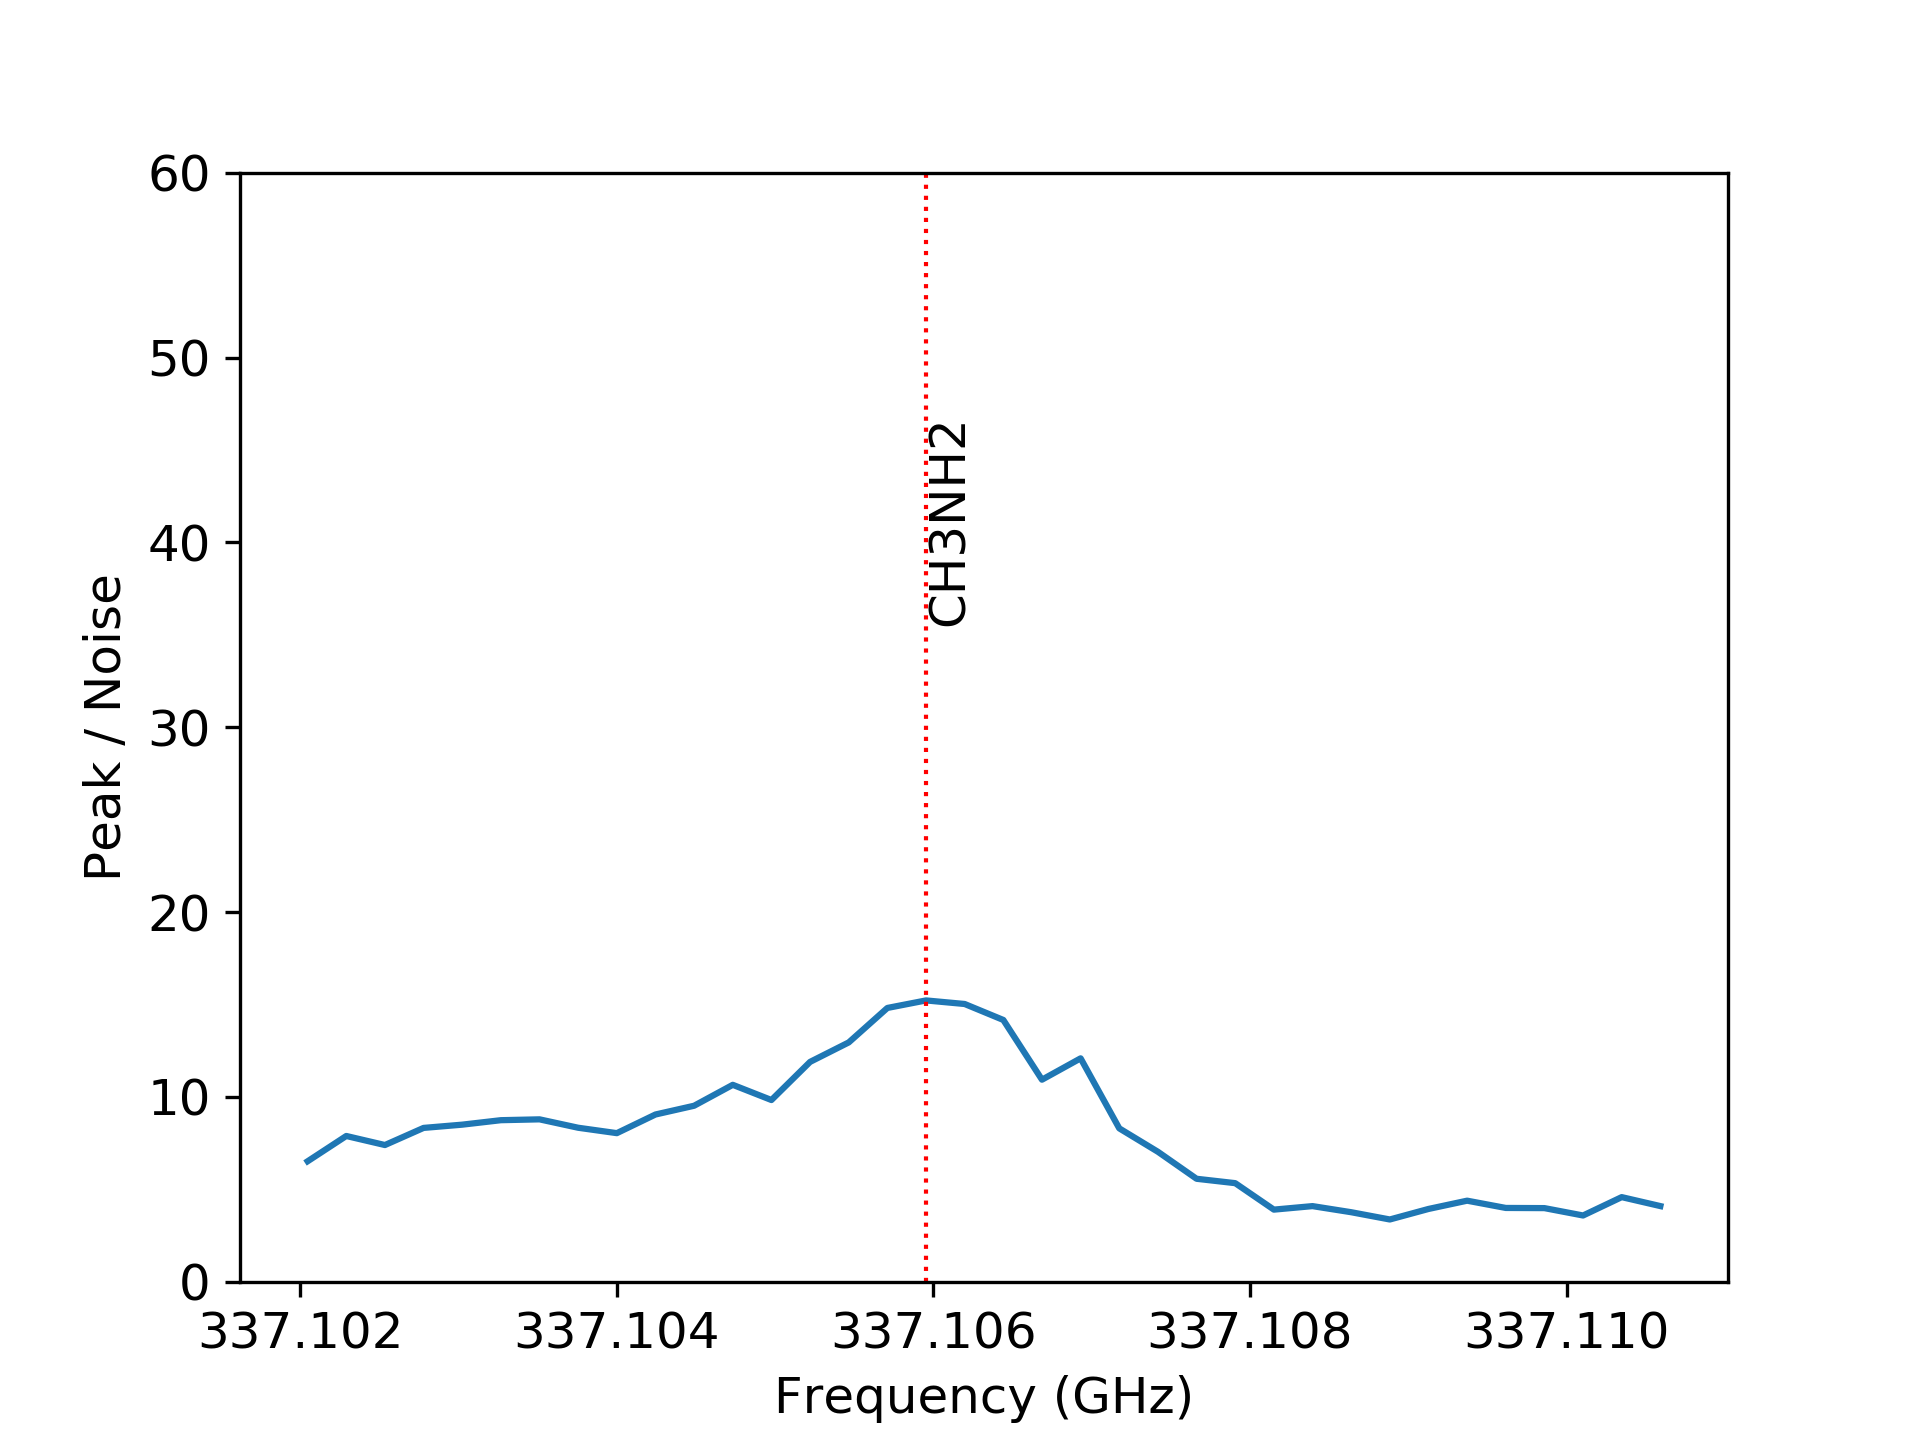
\includegraphics[width=0.33\textwidth]{spw0_CH3NH2}
    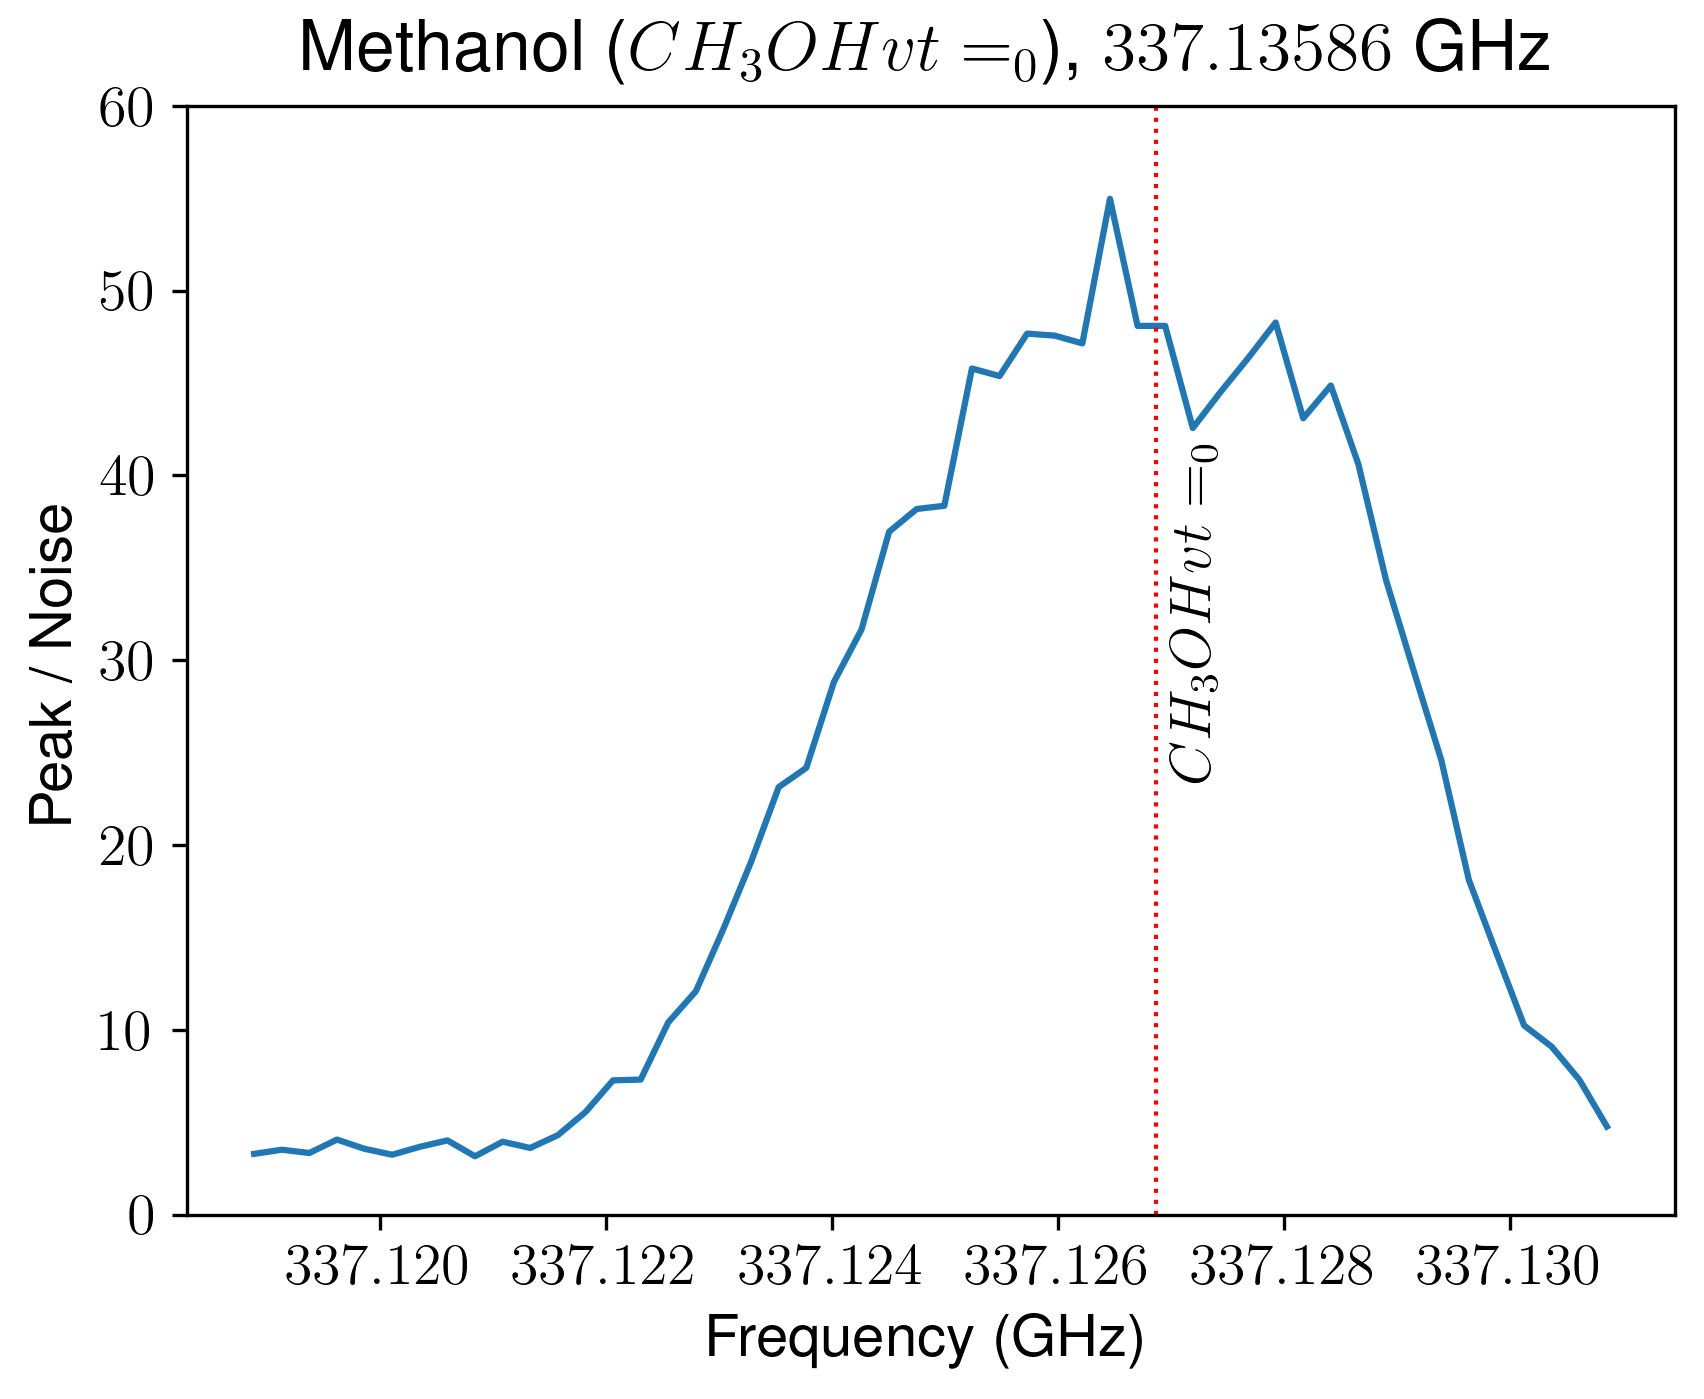
\includegraphics[width=0.33\textwidth]{spw0_CH3OHvt=0}
    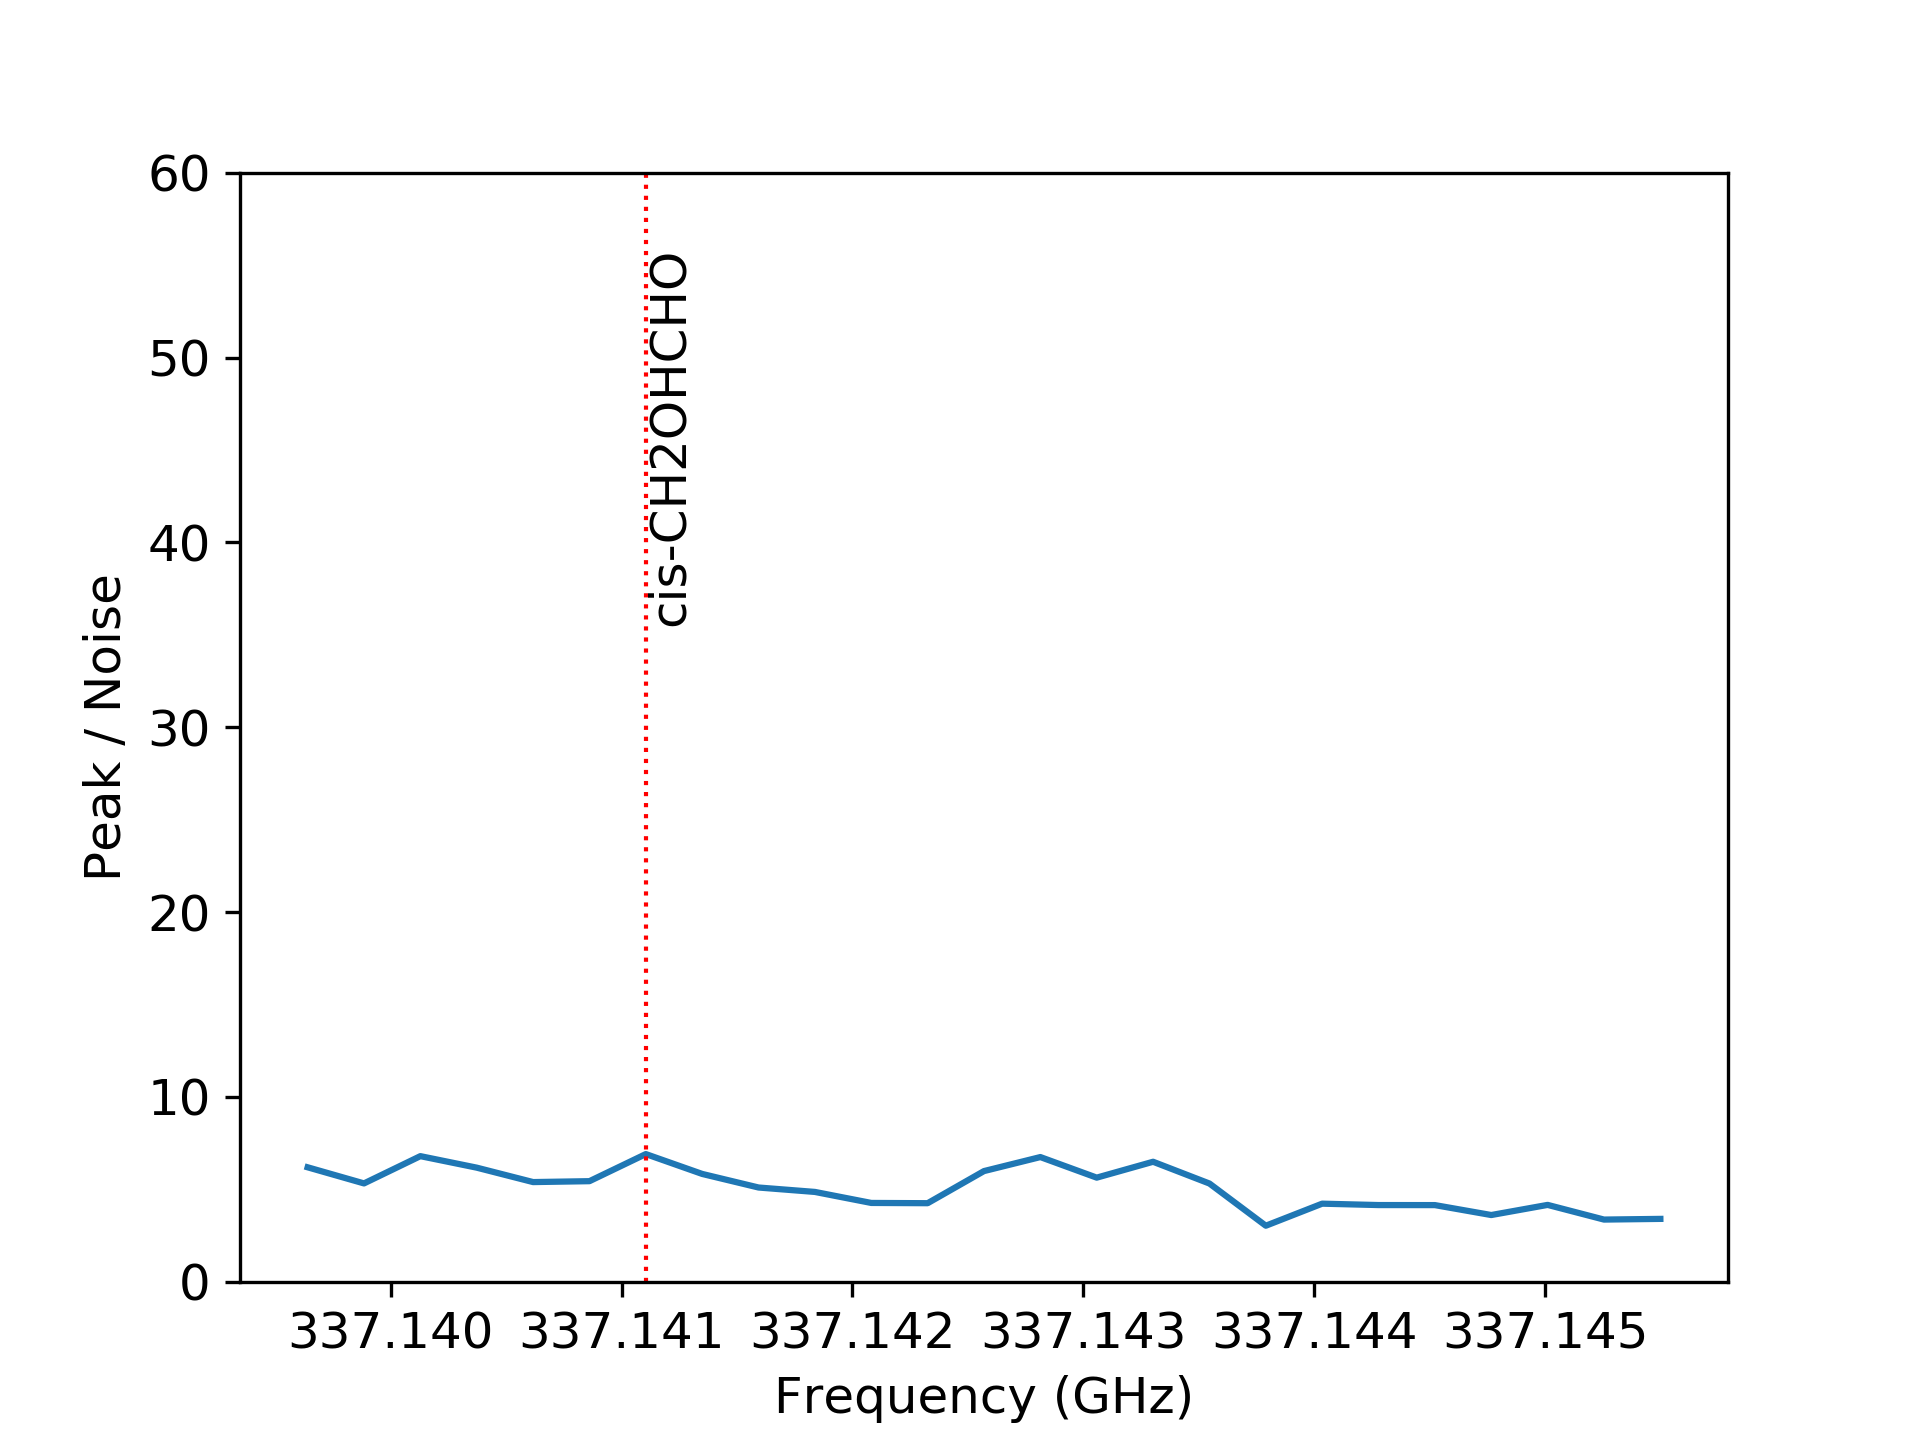
\includegraphics[width=0.33\textwidth]{spw0_cis-CH2OHCHO}
    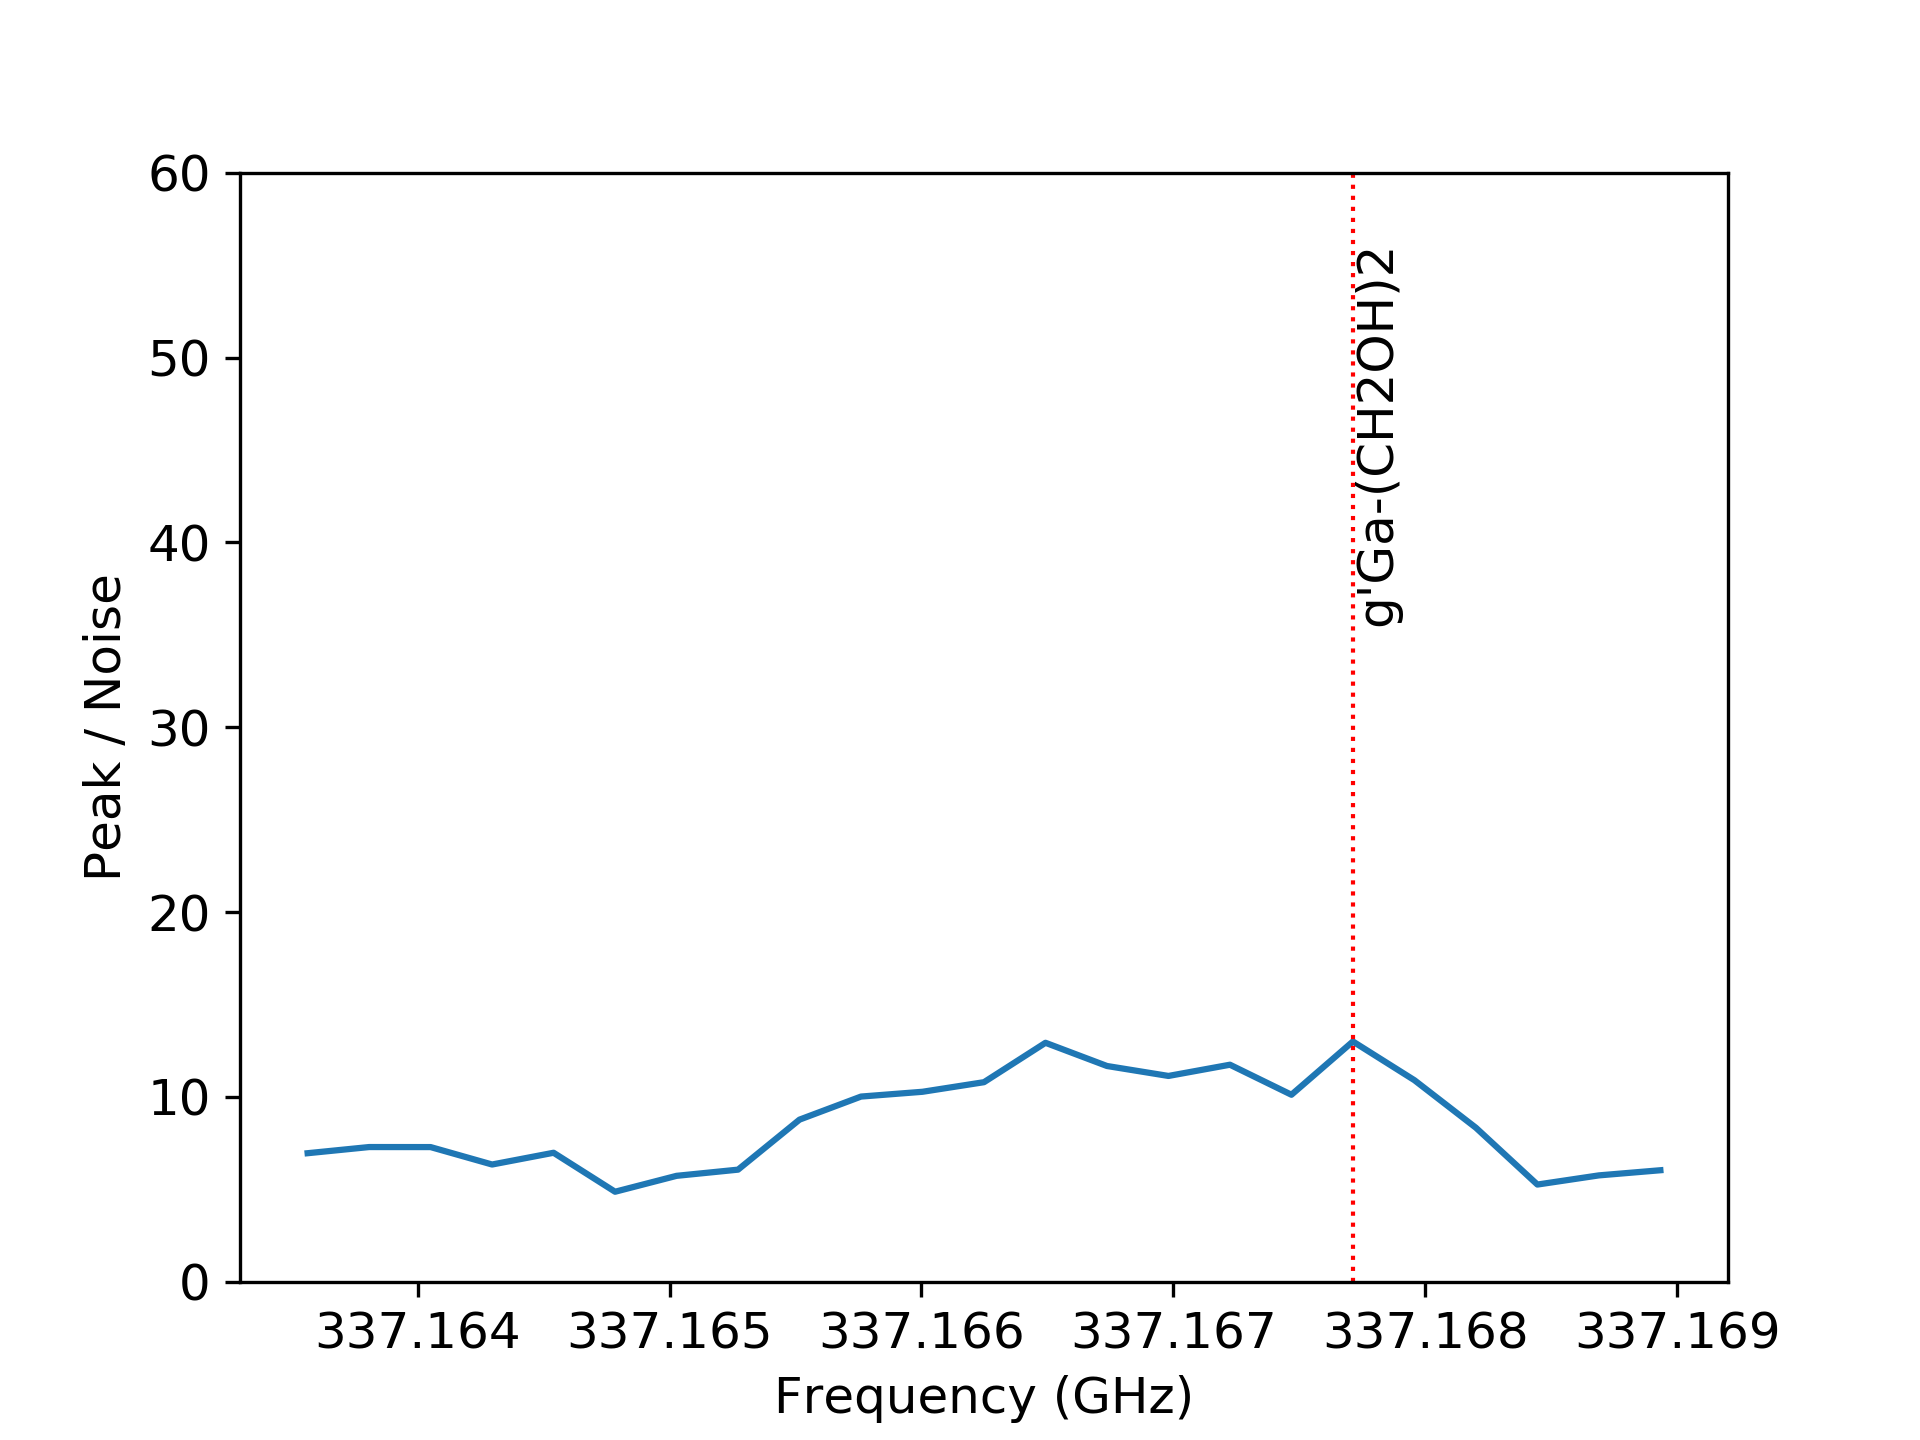
\includegraphics[width=0.33\textwidth]{spw0_g'Ga-(CH2OH)2}
    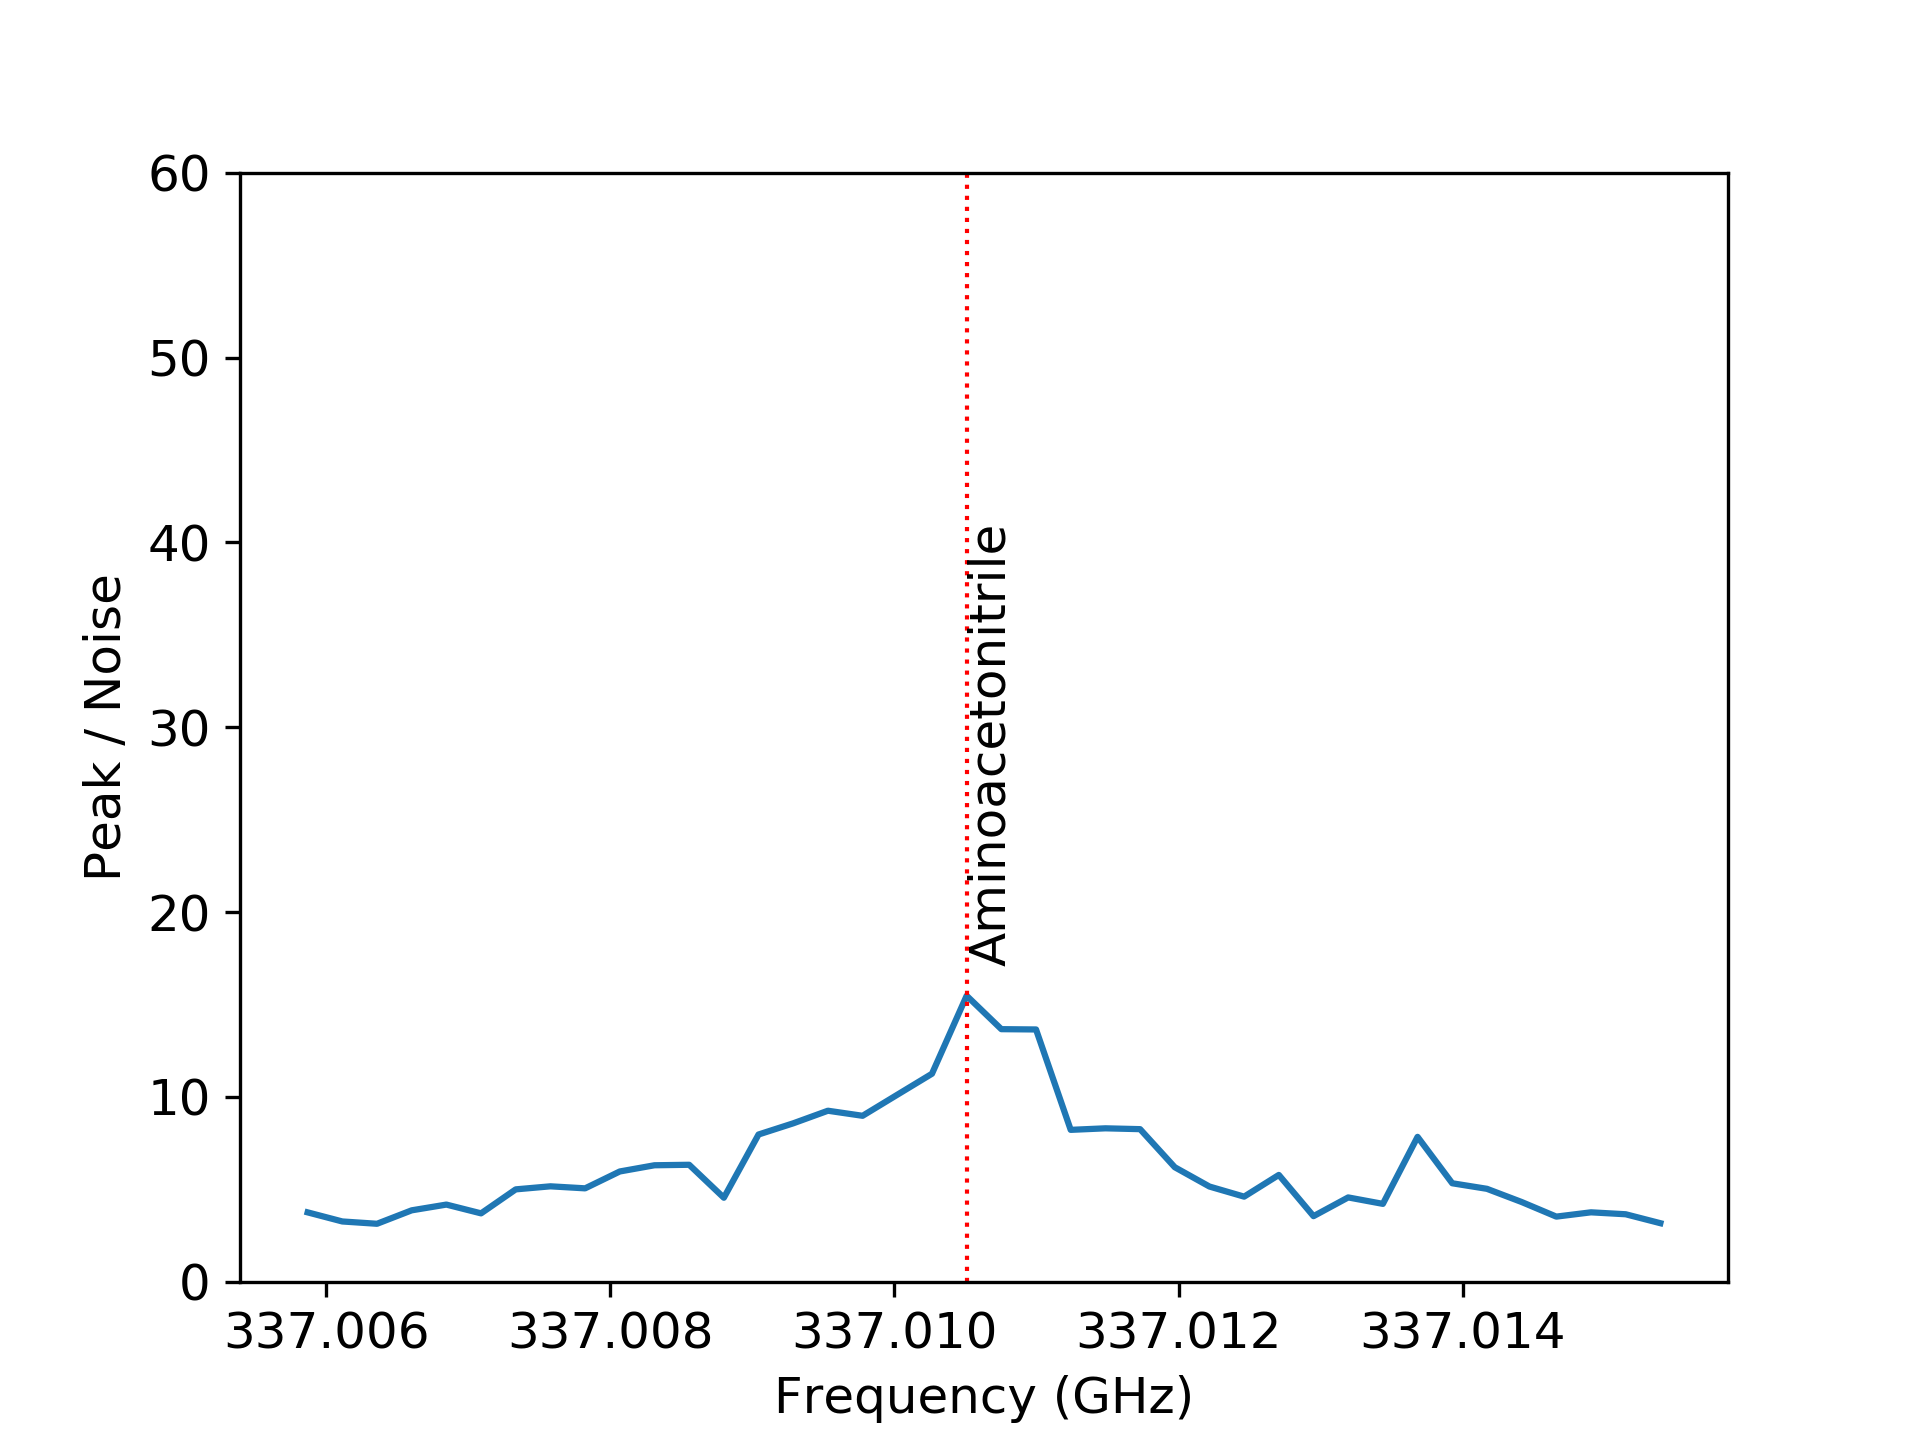
\includegraphics[width=0.33\textwidth]{spw0_H2NCH2CN}
    \caption{Promising molecular lines identified in spectral window 0}
   \end{figure*}

\begin{table*}   
 \label{table:2}  
    \caption{Line identification results for spectral window 1}
    \tiny
    \centering    
    \begin{tabular}{l l l l l l l l l} 
    \hline     
    Molecule & Name &Transition & Frequency & $E_{u}$ & Intensity & Velocity & $v_{lsr}$ & Peak / rms\\ 
    \hline
$CH_{3}OHvt=_{0}$ & Methanol & $14_{7,8}-15_{6,9}++$ & $336.43822$ & $488.2179$ & $3.3687$ & $7.3909$ & $8.0$ & $3.1028$\\
$CNCHO$ & Cyanoformaldehyde & $35_{6,30}-36_{5,31}$ & $336.44841$ & $400.3188$ & $2.7454$ & $7.0118$ & $8.0$ & $2.5287$\\
$CH_{313}CH_{2}CN$ & Ethyl Cyanide & $34_{8,26}-34_{7,27}$ & $336.45107$ & $323.9327$ & $0.6648$ & $8.7744$ & $8.0$ & $1.7433$\\
$CH_{3}OCHO$ & Methyl Formate & $35_{13,23}-35_{12,24}A$ & $336.45452$ & $484.8088$ & $2.9014$ & $6.3529$ & $8.0$ & $2.6725$\\
$CH_{3}OCHO$ & Methyl Formate & $35_{13,22}-35_{12,23}E$ & $336.46561$ & $484.8108$ & $1.7567$ & $7.9995$ & $8.0$ & $4.6065$\\
$CNCHO$ & Cyanoformaldehyde & $35_{6,29}-36_{5,32}$ & $336.46699$ & $400.3188$ & $3.3371$ & $6.9874$ & $8.0$ & $3.0738$\\
$HC_{3}N$ & Cyanoacetylene & $J=37-36$ & $336.52008$ & $306.905$ & $8.053$ & $13.4069$ & $8.0$ & $21.1174$\\
$CCCO$ & 3-Oxo-1,2-Propadienylidene & $35-34$ & $336.62937$ & $290.8558$ & $-0.3128$ & $12.6003$ & $8.0$ & $-0.8202$\\
$(CH_{3})_{2}CO$ & Acetone & $23_{13,10}-22_{14,9}EA$ & $336.64028$ & $222.2164$ & $-13.5255$ & $10.0258$ & $8.0$ & $-12.458$\\
$H_{2}NCH_{2}CN$ & Aminoacetonitrile & $37_{19,18}-36_{19,17}$ & $336.65152$ & $748.4583$ & $-13.5255$ & $6.1625$ & $8.0$ & $-12.458$\\
$(CH_{3})_{2}CO$ & Acetone & $20_{13,8}-19_{12,7}AA$ & $336.65982$ & $171.7552$ & $-16.9879$ & $6.8598$ & $8.0$ & $-15.6472$\\
$SO_{2}$ & Sulfur dioxide & $16_{7,9}-17_{6,12}$ & $336.66958$ & $245.1142$ & $-13.0386$ & $7.5137$ & $8.0$ & $-12.0096$\\
    \hline                  
    \end{tabular}
\end{table*}

\newpage
   \begin{figure*}
    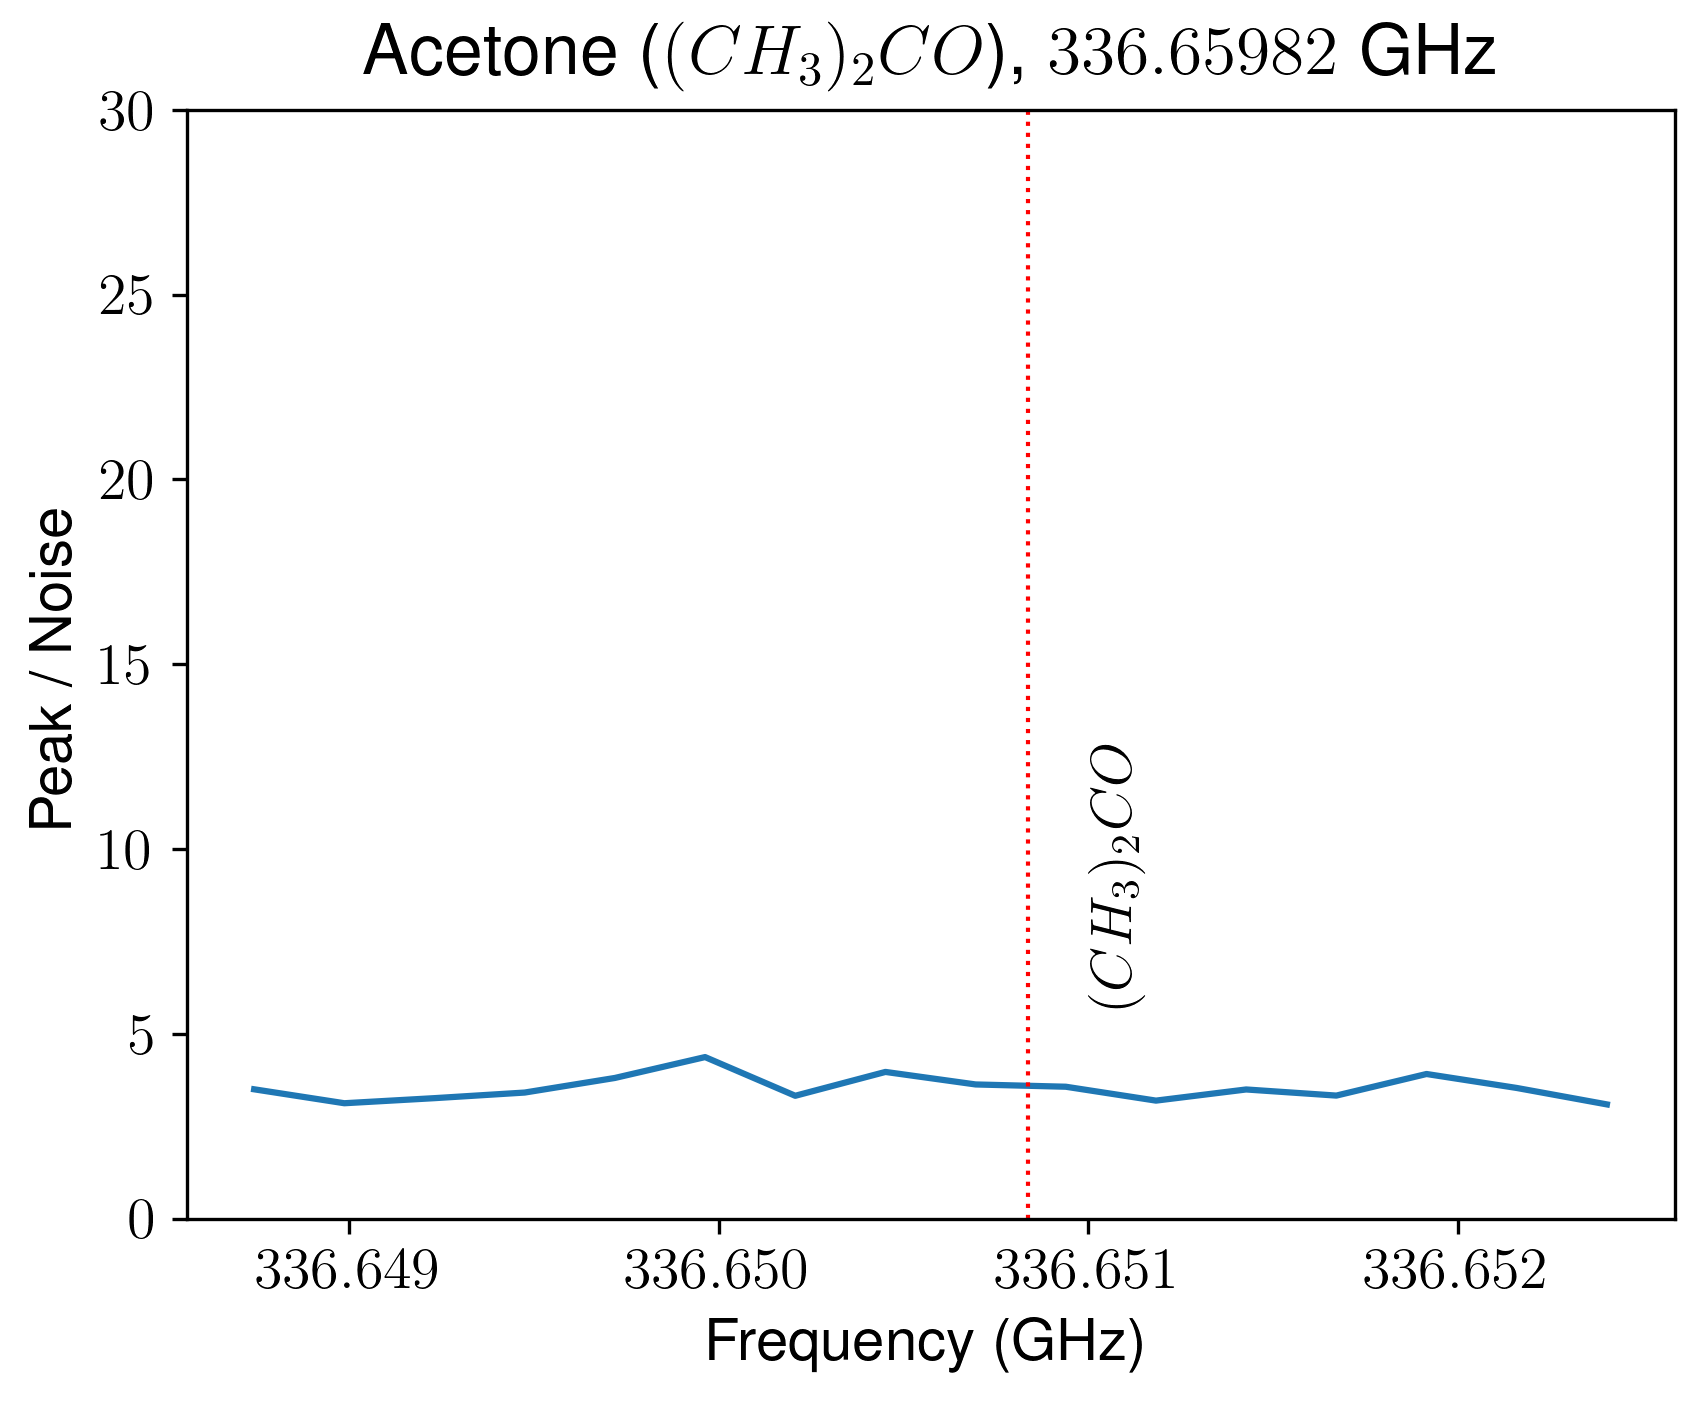
\includegraphics[width=0.33\textwidth]{spw1_(CH3)2CO}
    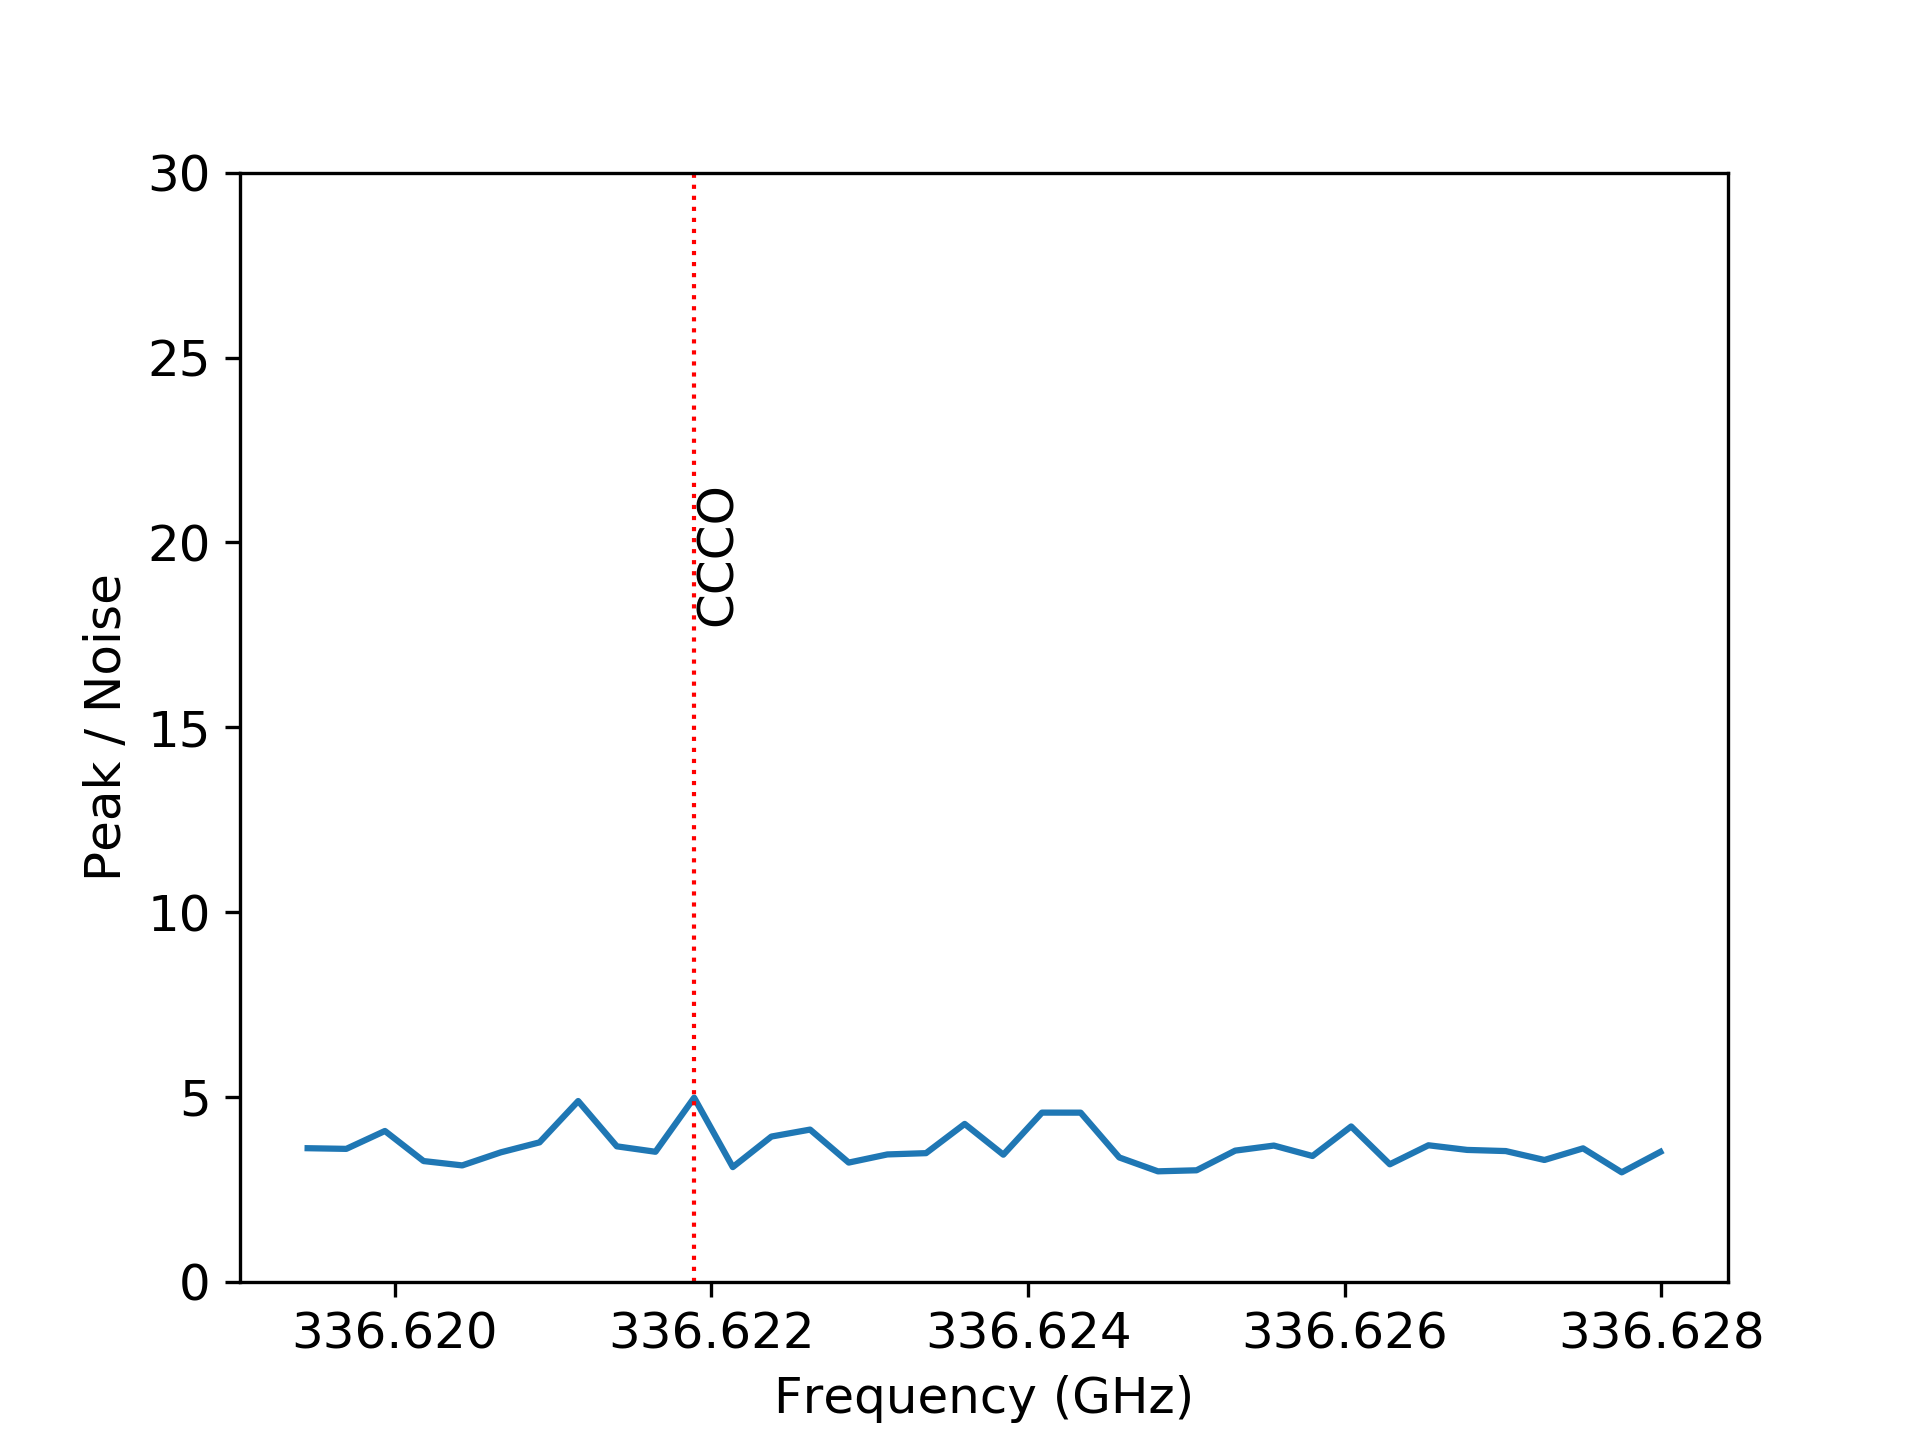
\includegraphics[width=0.33\textwidth]{spw1_CCCO}
    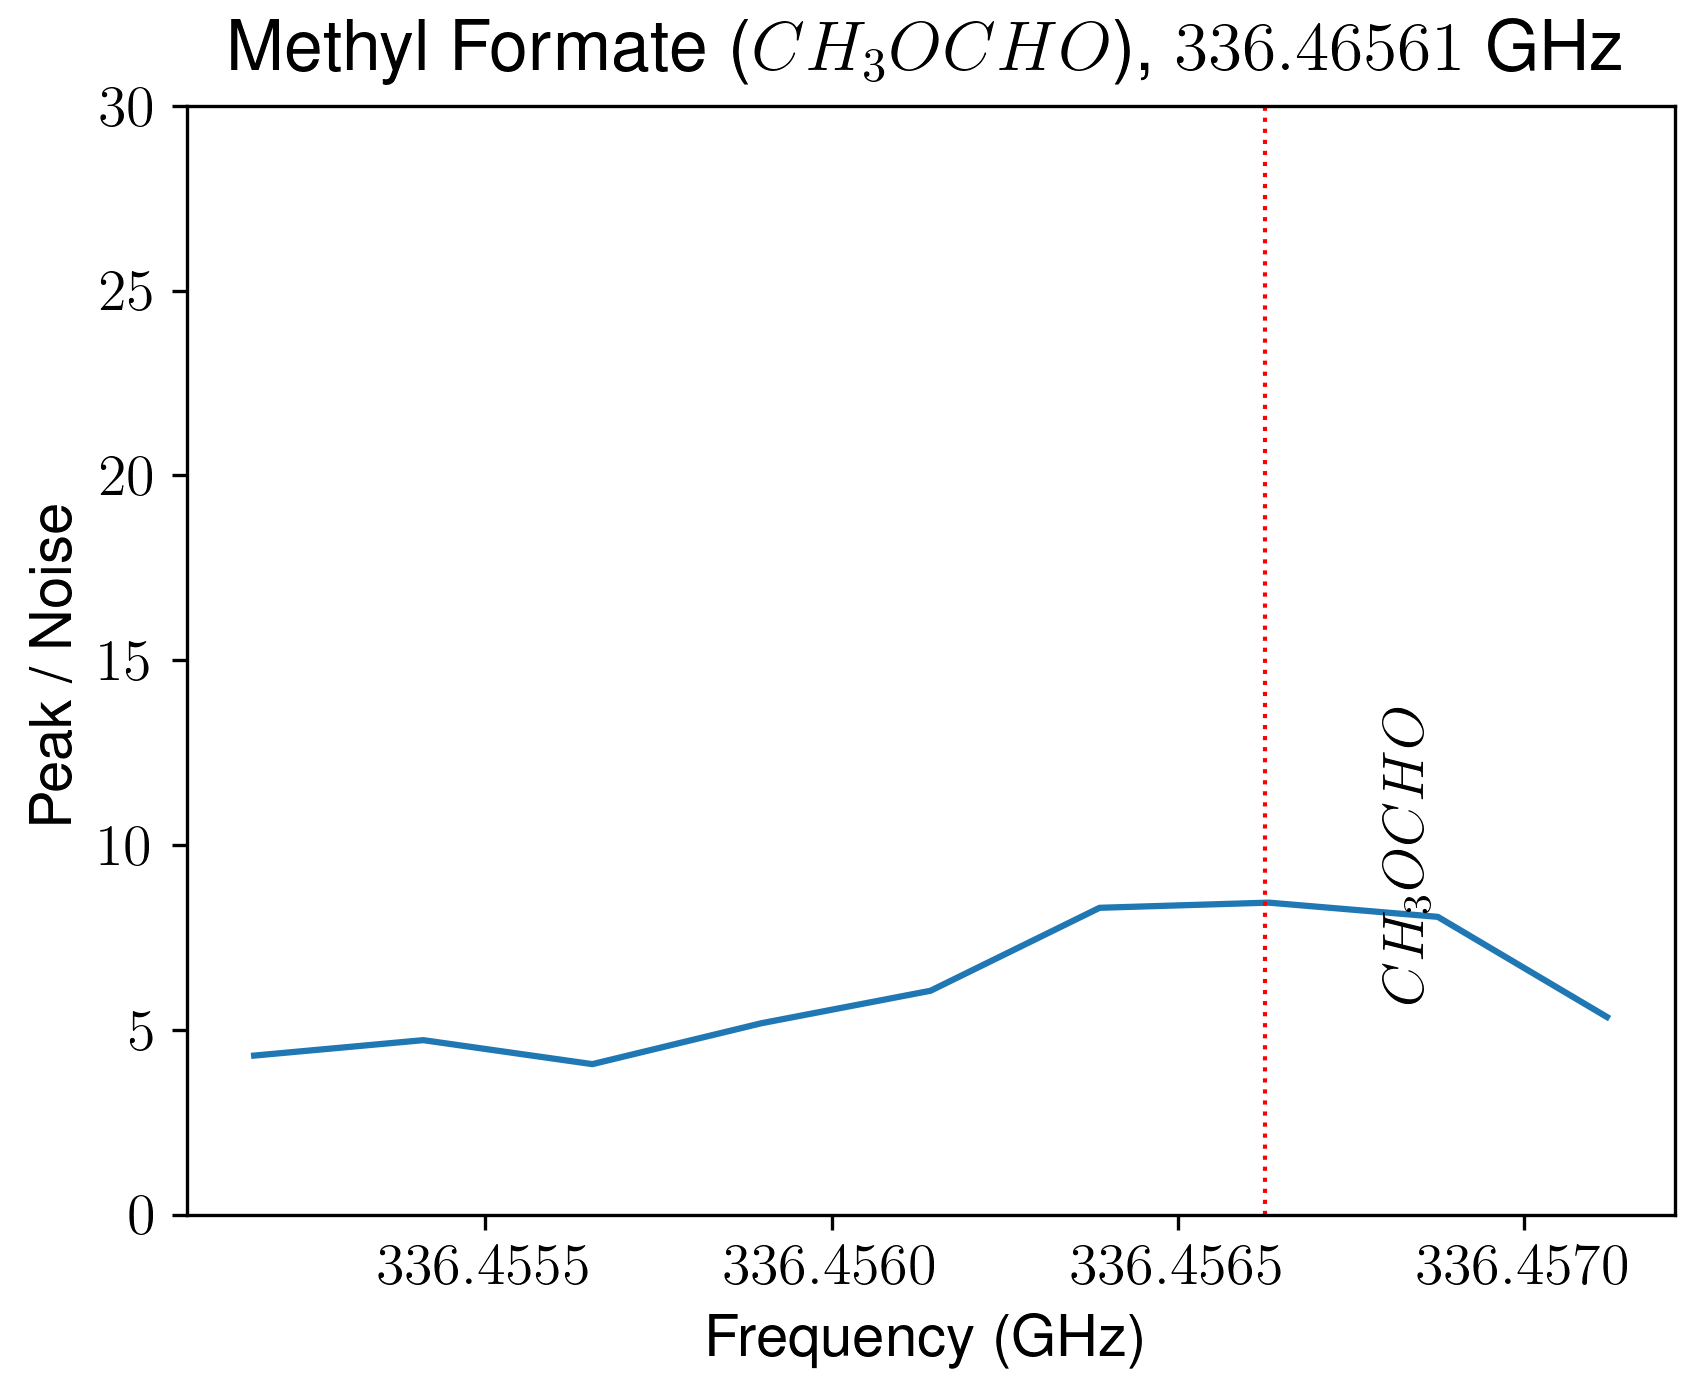
\includegraphics[width=0.33\textwidth]{spw1_CH3OCHO}
    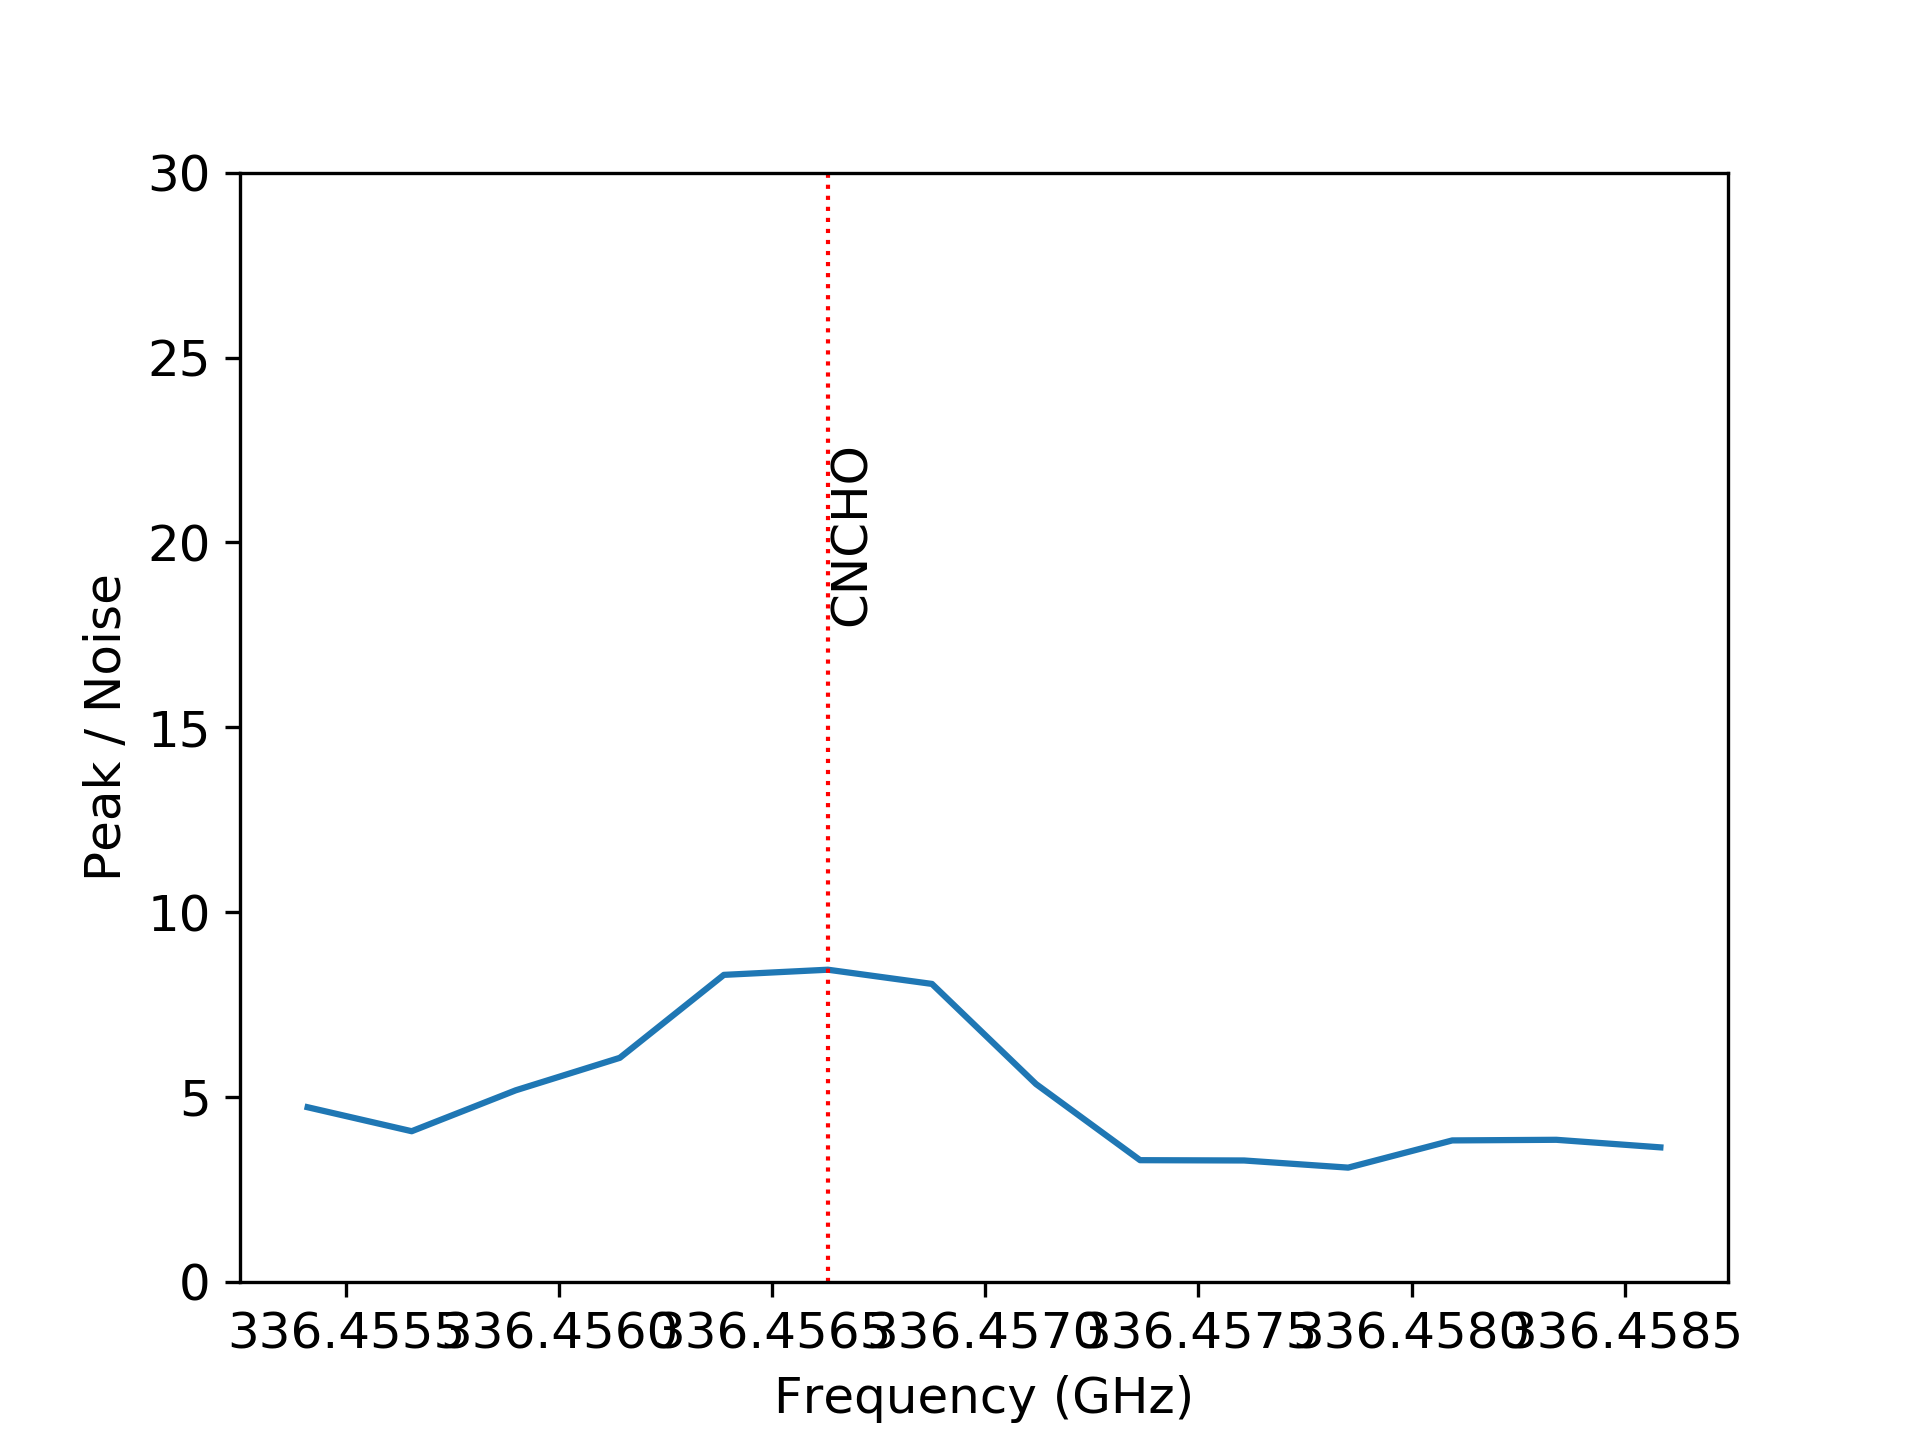
\includegraphics[width=0.33\textwidth]{spw1_CNCHO}
    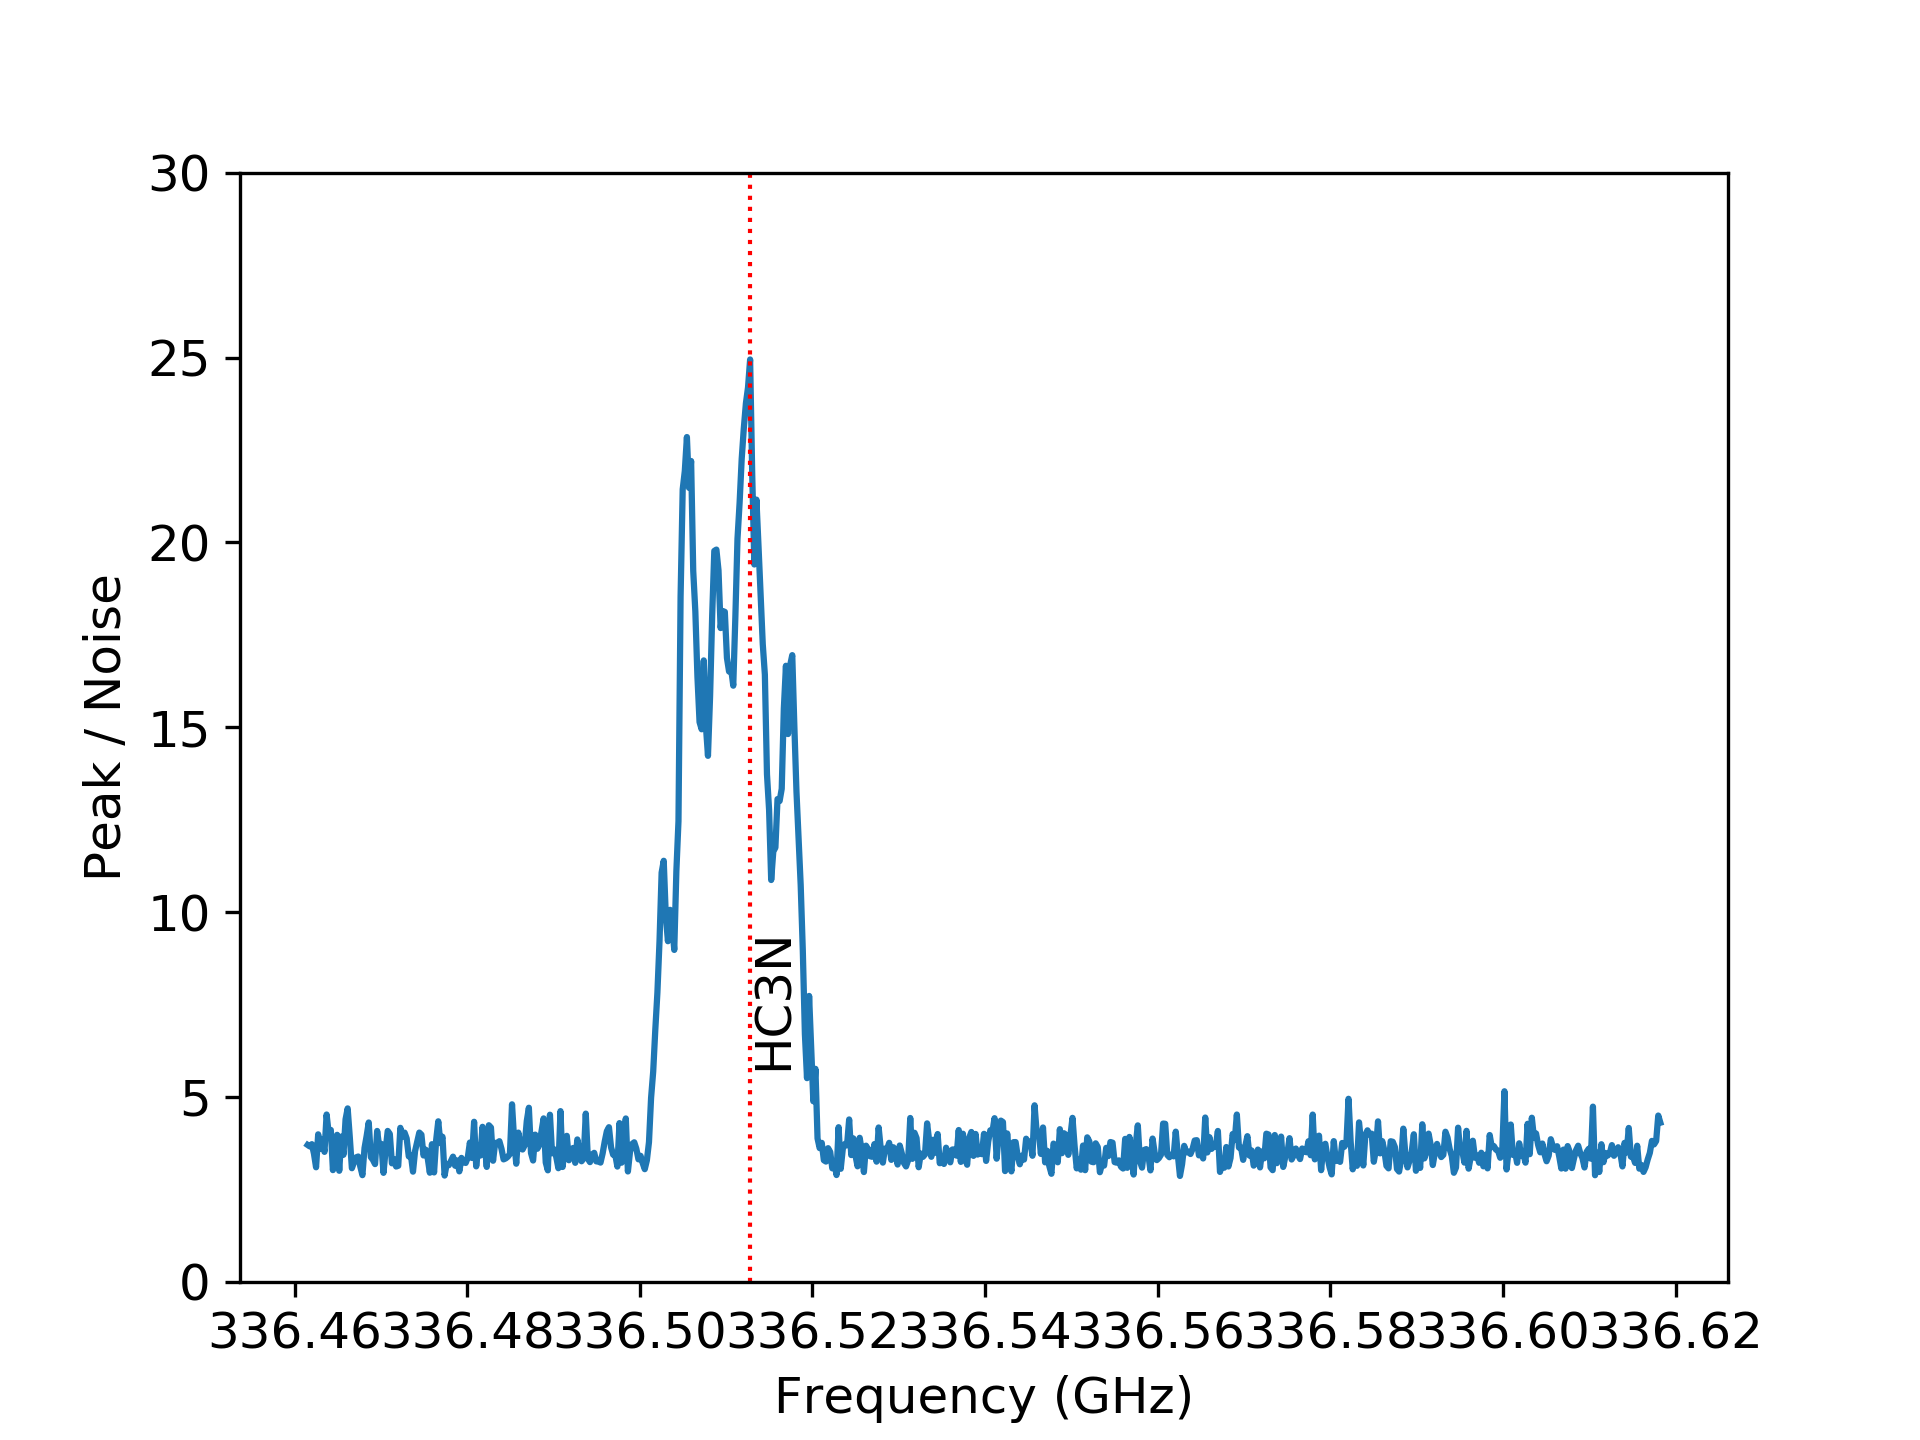
\includegraphics[width=0.33\textwidth]{spw1_HC3N}
    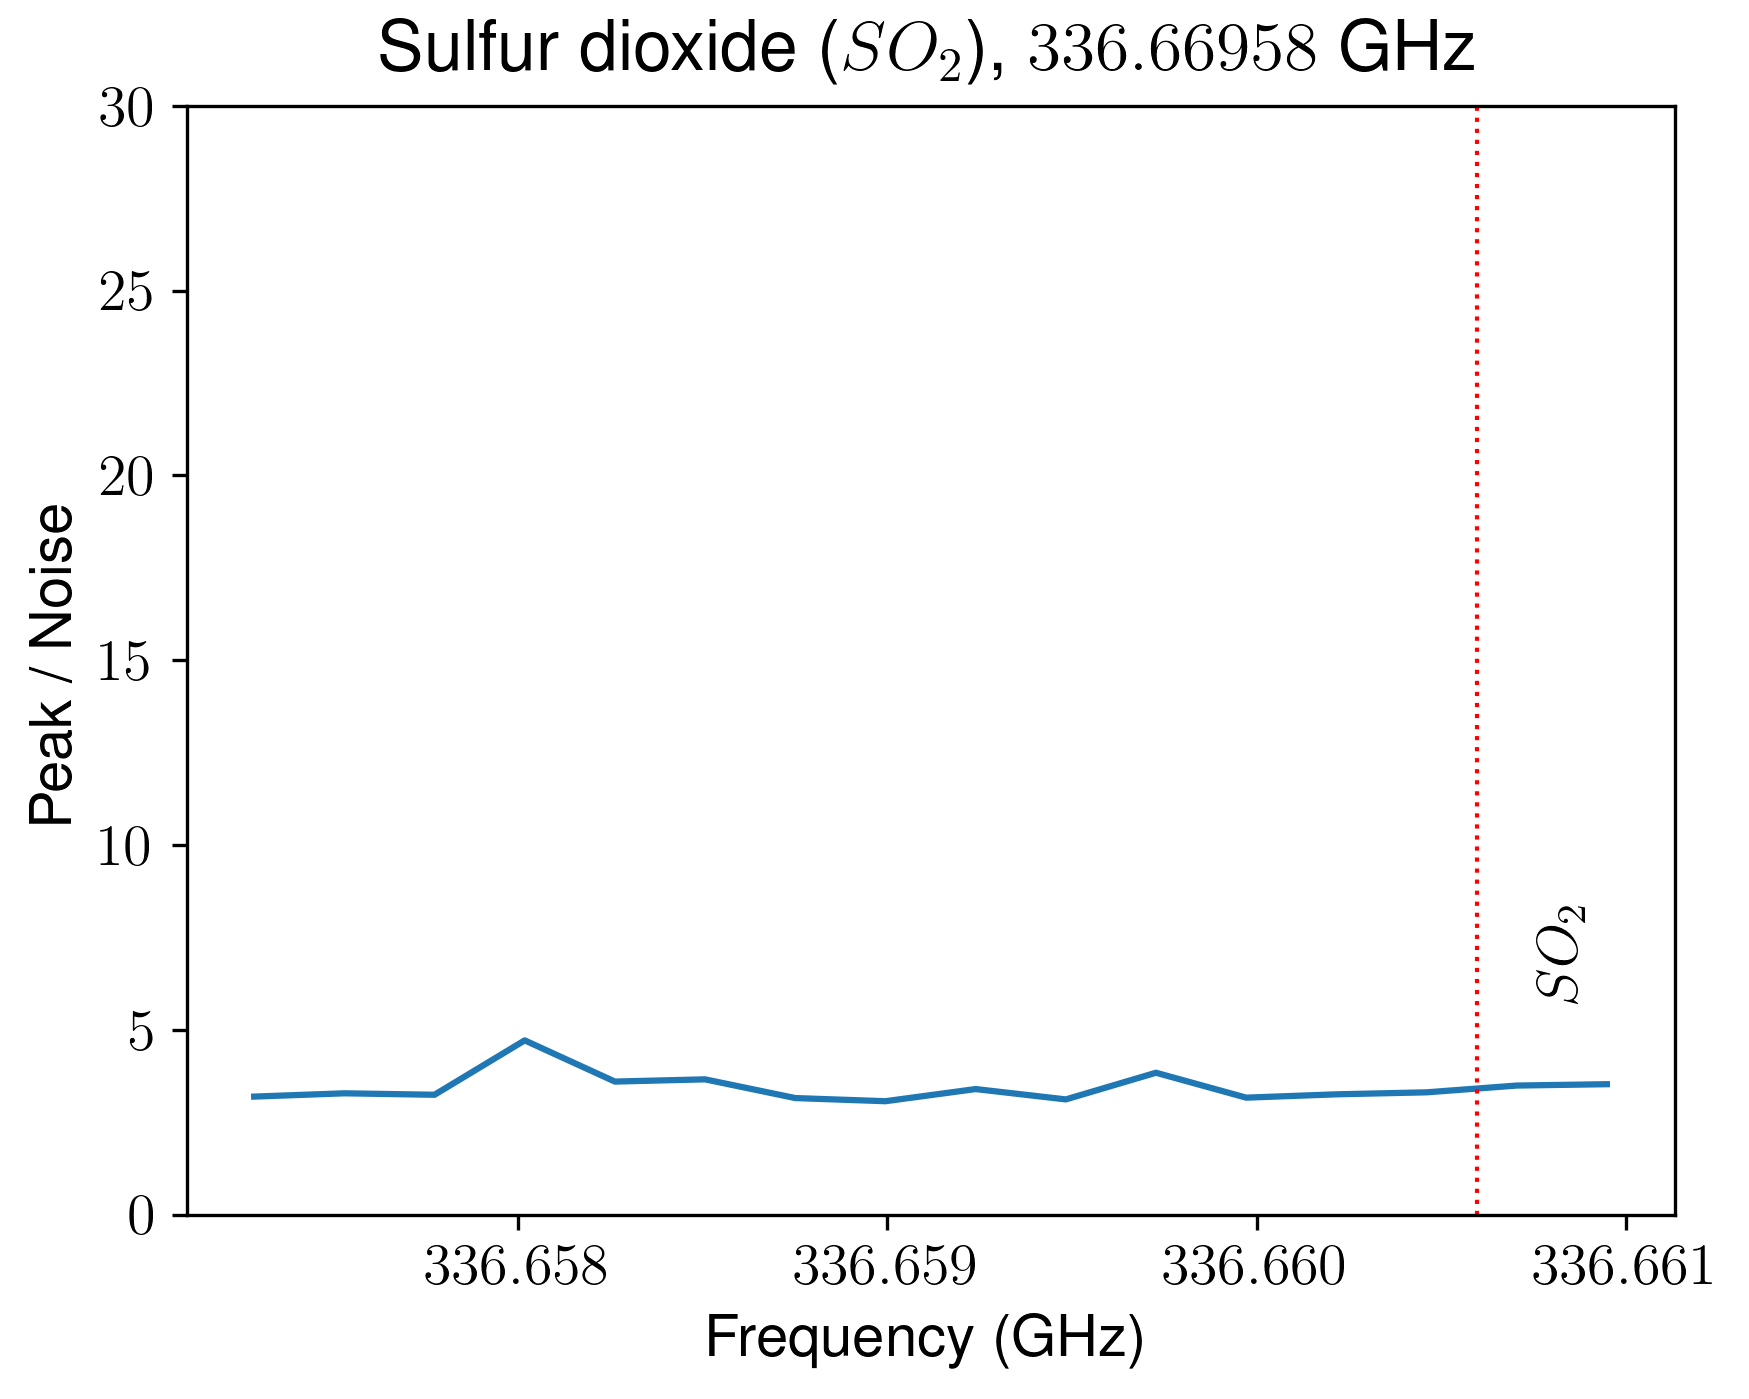
\includegraphics[width=0.33\textwidth]{spw1_SO2}
    \caption{Promising molecular lines identified in spectral window 1}
   \end{figure*}


   \begin{table*}   
 \label{table:3}  
    \caption{Line identification results for spectral window 2}
    \tiny
    \centering    
    \begin{tabular}{l l l l l l l l l} 
    \hline     
    Molecule & Name &Transition & Frequency & $E_{u}$ & Intensity & Velocity & $v_{lsr}$ & Peak / rms\\ 
    \hline
$cis-CH_{2}OHCHO$ & Glycolaldehyde & $7_{6,2}-6_{4,3}$ & $334.05821$ & $37.4116$ & $45.0294$ & $6.5106$ & $8.0$ & $50.0827$\\
$CH_{3}OCHO$ & Methyl Formate & $15_{6,10}-14_{5,9}A$ & $334.10909$ & $94.8964$ & $17.0495$ & $9.9217$ & $8.0$ & $18.9629$\\
$CH_{3}NH_{2}$ & Methylamine & $17_{2}E1+1-17_{1}E1-1$ & $334.13094$ & $342.265$ & $10.4351$ & $14.8478$ & $8.0$ & $11.6061$\\
$_{33}SO_{2}$ & Sulfur Dioxide & $36_{11,25}-37_{10,28},F=69/2-71/2$ & $334.14626$ & $915.5991$ & $-0.6228$ & $8.9463$ & $8.0$ & $-1.4553$\\
$t-CH_{2}CHCHO$ & Propenal & $9_{3,7}-9_{1,8}$ & $334.20301$ & $37.7617$ & $3.1656$ & $6.2555$ & $8.0$ & $3.5209$\\
$CH_{3}NH_{2}$ & Methylamine & $8_{5}B1-9_{4}B2$ & $334.20979$ & $174.0493$ & $3.9923$ & $8.9327$ & $8.0$ & $4.4404$\\
$(CH_{3})_{2}CO$ & Acetone & $13_{11,3}-12_{8,4}AA$ & $334.21979$ & $80.4654$ & $-0.4388$ & $7.6194$ & $8.0$ & $-1.0253$\\
$CH_{3}OCHO$ & Methyl Formate & $29_{5,24}-28_{6,23}A$ & $334.23598$ & $282.1007$ & $3.9697$ & $1.2063$ & $8.0$ & $4.4152$\\
$_{13}CH_{3}OHvt=_{0}$ & Methanol & $3_{2,1}-2_{0,2}$ & $334.25221$ & $35.9468$ & $3.4457$ & $9.4204$ & $8.0$ & $3.8324$\\
$CP$ & Carbon Monophosphide & $N=7-6,J=15/2-13/2,F=8-7$ & $334.26182$ & $64.2111$ & $45.3174$ & $11.3104$ & $8.0$ & $50.4031$\\
$CH_{3}OCHO$ & Methyl Formate & $15_{6,9}-14_{5,9}E$ & $334.28144$ & $94.9147$ & $13.9904$ & $12.98$ & $8.0$ & $15.5604$\\
$g'Ga-(CH_{2}OH)_{2}$ & Ethylene Glycol & $15_{9,7}v=1-14_{8,7}v=0$ & $334.30955$ & $99.0907$ & $4.2402$ & $7.0359$ & $8.0$ & $4.7161$\\
$CH_{3}OHvt=_{1}$ & Methanol & $21_{5,16}-22_{4,19}$ & $334.32728$ & $964.3871$ & $6.4237$ & $12.1515$ & $8.0$ & $7.1446$\\
$s-H_{2}CCHOH$ & Vinyl Alcohol & $17_{4,13}-16_{4,12}$ & $334.34291$ & $182.2279$ & $15.4923$ & $6.892$ & $8.0$ & $17.2309$\\
$CH_{3}COOH$ & Acetic Acid & $30_{*,29}-29_{*,28}v=0$ & $334.37851$ & $259.444$ & $4.3631$ & $-4.0152$ & $8.0$ & $4.8527$\\
$g'Ga-(CH_{2}OH)_{2}$ & Ethylene Glycol & $24_{6,19}v=0-23_{5,18}v=0$ & $334.41275$ & $165.9969$ & $45.6615$ & $10.8101$ & $8.0$ & $50.7858$\\
$CH_{3}OHvt=_{1}$ & Methanol & $3_{0,3}-2_{1,2}$ & $334.42656$ & $314.4694$ & $52.4693$ & $7.1835$ & $8.0$ & $58.3575$\\
$g'Ga-(CH_{2}OH)_{2}$ & Ethylene Glycol & $13_{10,4}v=1-12_{9,4}v=0$ & $334.46125$ & $94.1713$ & $44.2048$ & $-2.9053$ & $8.0$ & $49.1656$\\
$(CH_{3})_{2}CO$ & Acetone & $13_{11,2}-12_{8,4}EE$ & $334.58973$ & $80.5543$ & $8.5715$ & $-10.7174$ & $8.0$ & $9.5334$\\
$t-CH_{3}CH_{2}OH$ & trans-Ethanol & $24_{7,17}-24_{6,18}$ & $334.60263$ & $313.8344$ & $12.3572$ & $5.1576$ & $8.0$ & $13.7439$\\
$CH_{3}OHvt=_{1}$ & Methanol & $22_{3,20}-22_{2,21}$ & $334.63249$ & $1001.3148$ & $13.0942$ & $11.6487$ & $8.0$ & $14.5637$\\
$CH_{3}OHvt=_{1}$ & Methanol & $25_{-3,22}-24_{-2,22}$ & $334.67771$ & $1073.8453$ & $21.2092$ & $-0.8691$ & $8.0$ & $23.5894$\\
$CH_{3}NH_{2}$ & Methylamine & $2_{2}A2-1_{1}A1,F=2-1$ & $334.71119$ & $22.5092$ & $0.0$ & $0.0$ & $8.0$ & $0.0$\\
$CCO$ & Oxoethenylidene & $N=14-13,J=14-14$ & $334.75876$ & $116.8058$ & $12.7521$ & $-3.4945$ & $8.0$ & $14.1832$\\
$(CH_{3})_{2}CO$ & Acetone & $12_{8,4}-11_{5,7}AE$ & $334.76545$ & $64.565$ & $20.6655$ & $11.5016$ & $8.0$ & $22.9846$\\
$CH_{3}CHO$ & Acetaldehyde & $17_{2,15}-16_{2,14}A++$ & $334.93139$ & $152.6118$ & $43.1424$ & $6.3067$ & $8.0$ & $47.9839$\\
$H_{213}CS$ & Thioformaldehyde & $10_{1,9}-9_{1,8}$ & $334.94932$ & $101.6033$ & $7.7273$ & $9.4859$ & $8.0$ & $8.5944$\\
$(CH_{3})_{2}CO$ & Acetone & $12_{8,4}-11_{5,7}EE$ & $334.99117$ & $64.4966$ & $13.4849$ & $-0.0038$ & $8.0$ & $14.9982$\\
$g'Ga-(CH_{2}OH)_{2}$ & Ethylene Glycol & $41_{17,24}v=0-41_{16,25}v=0$ & $335.07602$ & $565.0077$ & $0.462$ & $10.367$ & $8.0$ & $1.0795$\\
$c-H_{13}CCCH$ & Cyclopropenylidene & $5_{3,2}-5_{0,5}$ & $335.08781$ & $43.7198$ & $83.5866$ & $13.1283$ & $8.0$ & $92.9669$\\
$CH_{3}OHvt=_{0}$ & Methanol & $2_{2,1}-3_{1,2}--$ & $335.13369$ & $44.6721$ & $77.7538$ & $7.0251$ & $8.0$ & $86.4796$\\
$CH_{3}OCHO$ & Methyl Formate & $28_{4,24}-27_{5,23}A$ & $335.18332$ & $257.0799$ & $2.4819$ & $9.7965$ & $8.0$ & $2.7604$\\
$g-CH_{3}CH_{2}OH$ & gauche-Ethanol & $32_{6,27}-32_{5,27},vt=1-0$ & $335.2683$ & $545.844$ & $7.8166$ & $7.151$ & $8.0$ & $8.6938$\\
$CH_{3}CH_{2}CN$ & Ethyl Cyanide & $55_{8,48}-55_{7,49}$ & $335.27492$ & $733.8889$ & $7.8166$ & $8.2166$ & $8.0$ & $8.6938$\\
$HDO$ & Water & $3_{3,1}-4_{2,2}$ & $335.3955$ & $335.2672$ & $46.6299$ & $-58.3771$ & $8.0$ & $51.8628$\\
$HOCN$ & Cyanic acid & $16_{2,14}-15_{2,13}$ & $335.47103$ & $265.334$ & $3.6165$ & $14.814$ & $8.0$ & $4.0224$\\
$g-CH_{3}CH_{2}OH$ & gauche-Ethanol & $9_{4,5}-8_{3,6},vt=1-1$ & $335.48609$ & $118.6556$ & $39.5665$ & $1.356$ & $8.0$ & $44.0067$\\
$NHD_{2}$ & Ammonia & $1_{1,1}0s-0_{0,0}0s$ & $335.51385$ & $16.102$ & $47.0375$ & $68.9121$ & $8.0$ & $52.3161$\\
$CH_{3}OHvt=_{0}$ & Methanol & $7_{1,7}-6_{1,6}++$ & $335.58202$ & $78.9709$ & $56.2576$ & $-11.484$ & $8.0$ & $62.571$\\
$CH_{3}COOH$ & Acetic Acid & $15_{-15,0}-14_{-14,0}v=0$ & $335.60436$ & $128.6181$ & $10.8442$ & $-12.7636$ & $8.0$ & $12.0612$\\
$t-CH_{3}CH_{2}OH$ & trans-Ethanol & $23_{7,17}-23_{6,18}$ & $335.63059$ & $293.607$ & $17.1709$ & $8.6112$ & $8.0$ & $19.0979$\\
$cis-CH_{2}OHCHO$ & Glycolaldehyde & $21_{7,14}-21_{4,17}$ & $335.64676$ & $158.7973$ & $39.0976$ & $3.8067$ & $8.0$ & $43.4853$\\
$(CH_{3})_{2}CO$ & Acetone & $12_{11,1}-11_{8,4}EE$ & $335.67518$ & $71.4144$ & $24.4019$ & $8.8142$ & $8.0$ & $27.1404$\\
$cis-CH_{2}OHCHO$ & Glycolaldehyde & $68_{15,54}-68_{14,55}$ & $335.69367$ & $1456.6243$ & $-0.829$ & $8.4429$ & $8.0$ & $-1.9371$\\
$H_{2}NCH_{2}CN$ & Aminoacetonitrile & $21_{3,18}-20_{2,19}$ & $335.69558$ & $112.127$ & $-0.829$ & $6.7331$ & $8.0$ & $-1.9371$\\
$CH_{3}OHvt=_{0}$ & Methanol & $25_{8,17}-26_{7,20}++$ & $335.7015$ & $1073.9686$ & $0.0$ & $0.0$ & $8.0$ & $0.0$\\
$t-H_{13}COOH$ & Formic Acid & $6_{3,3}-7_{1,6}$ & $335.71489$ & $50.4224$ & $13.3501$ & $-0.5284$ & $8.0$ & $14.8482$\\
$CH_{3}NH_{2}$ & Methylamine & $14_{1}E1-1-13_{2}E1-1$ & $335.74509$ & $225.3446$ & $12.4894$ & $4.6287$ & $8.0$ & $13.8909$\\
$CH_{3}COOH$ & Acetic Acid & $13_{11,2}-12_{9,3}--v=0$ & $335.77985$ & $89.7941$ & $15.7797$ & $3.9964$ & $8.0$ & $17.5506$\\
$(CH_{3})_{2}CO$ & Acetone & $32_{2,30}-31_{3,29}EA$ & $335.80289$ & $281.4994$ & $0.0$ & $0.0$ & $8.0$ & $0.0$\\
$(CH_{3})_{2}CO$ & Acetone & $32_{2,30}-31_{2,29}AE$ & $335.80291$ & $281.4994$ & $11.5028$ & $1.213$ & $8.0$ & $12.7937$\\
$H_{2}C_{18}O$ & Formaldehyde & $5_{1,5}-4_{1,4}$ & $335.81594$ & $60.2335$ & $31.1124$ & $7.7668$ & $8.0$ & $34.6039$\\
$CH_{3}CH_{2}CN$ & Ethyl Cyanide & $10_{4,6}-10_{1,9}$ & $335.84026$ & $41.4386$ & $16.3359$ & $3.3581$ & $8.0$ & $18.1692$\\
$CH_{3}OCHO$ & Methyl Formate & $27_{9,19}-26_{9,17}E$ & $335.89969$ & $277.8455$ & $4.5668$ & $11.5288$ & $8.0$ & $5.0793$\\
    \hline                  
    \end{tabular}
\end{table*}


   \begin{figure*}
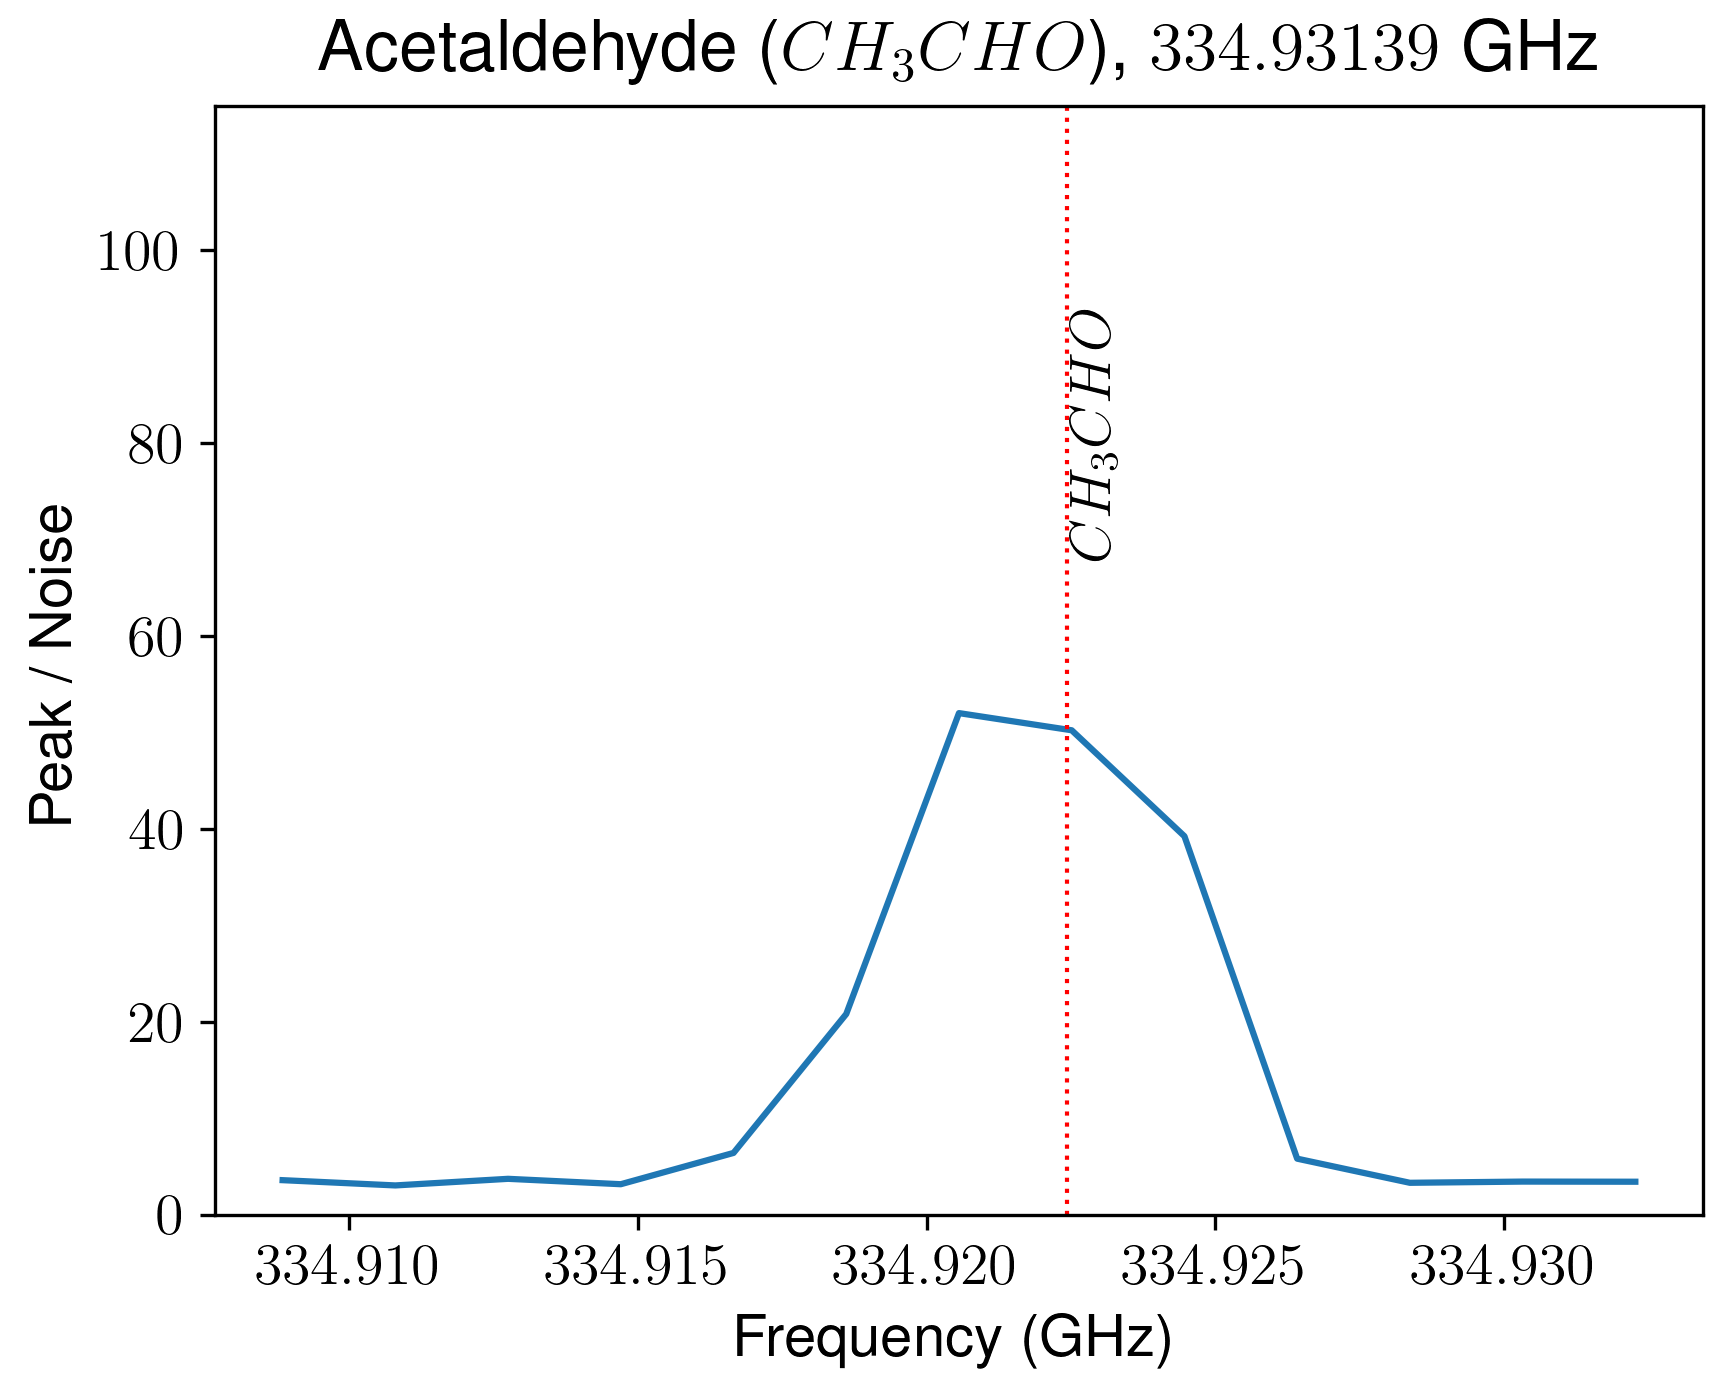
\includegraphics[width=0.33\textwidth]{spw2_CH3CHO}
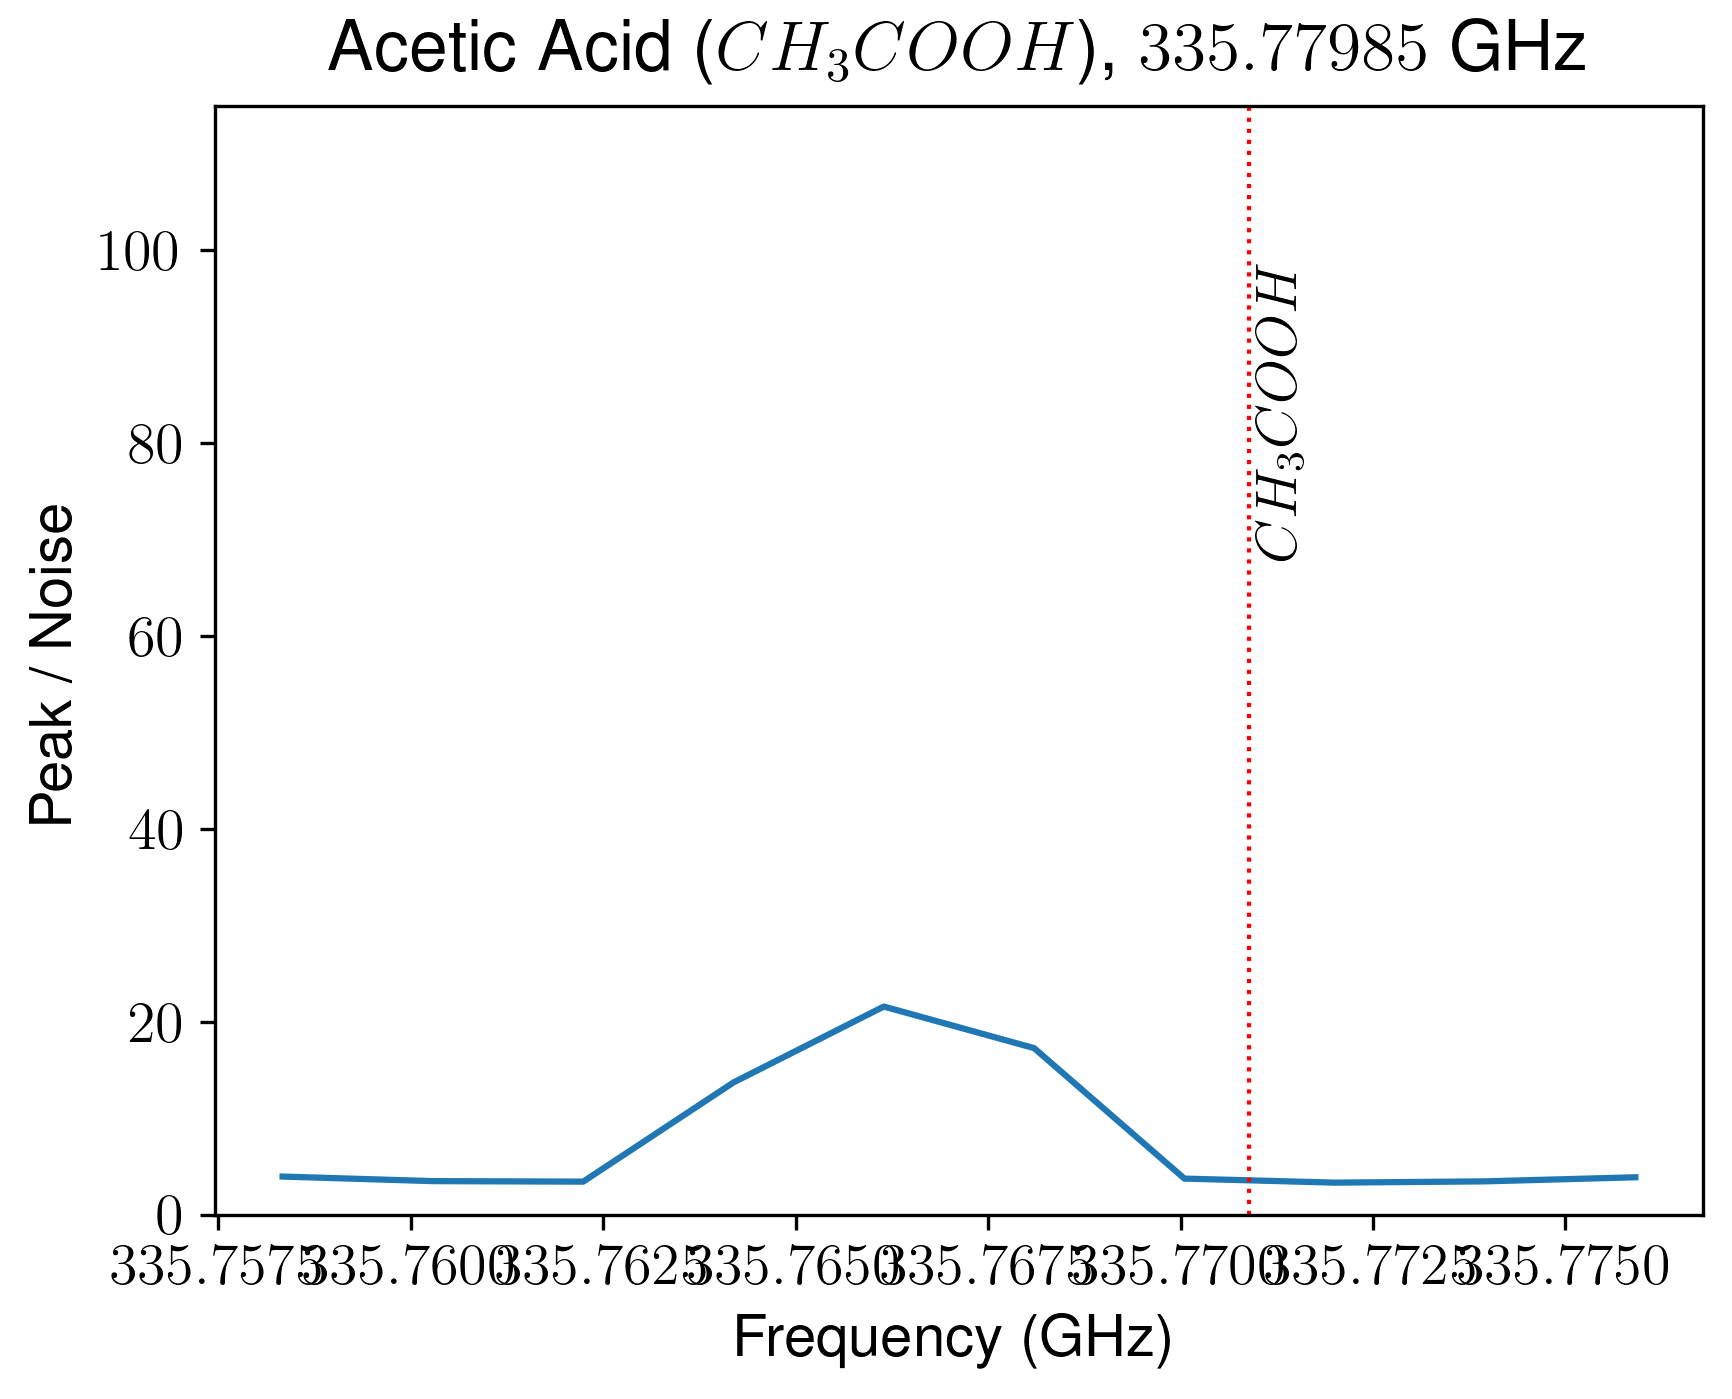
\includegraphics[width=0.33\textwidth]{spw2_CH3COOH}
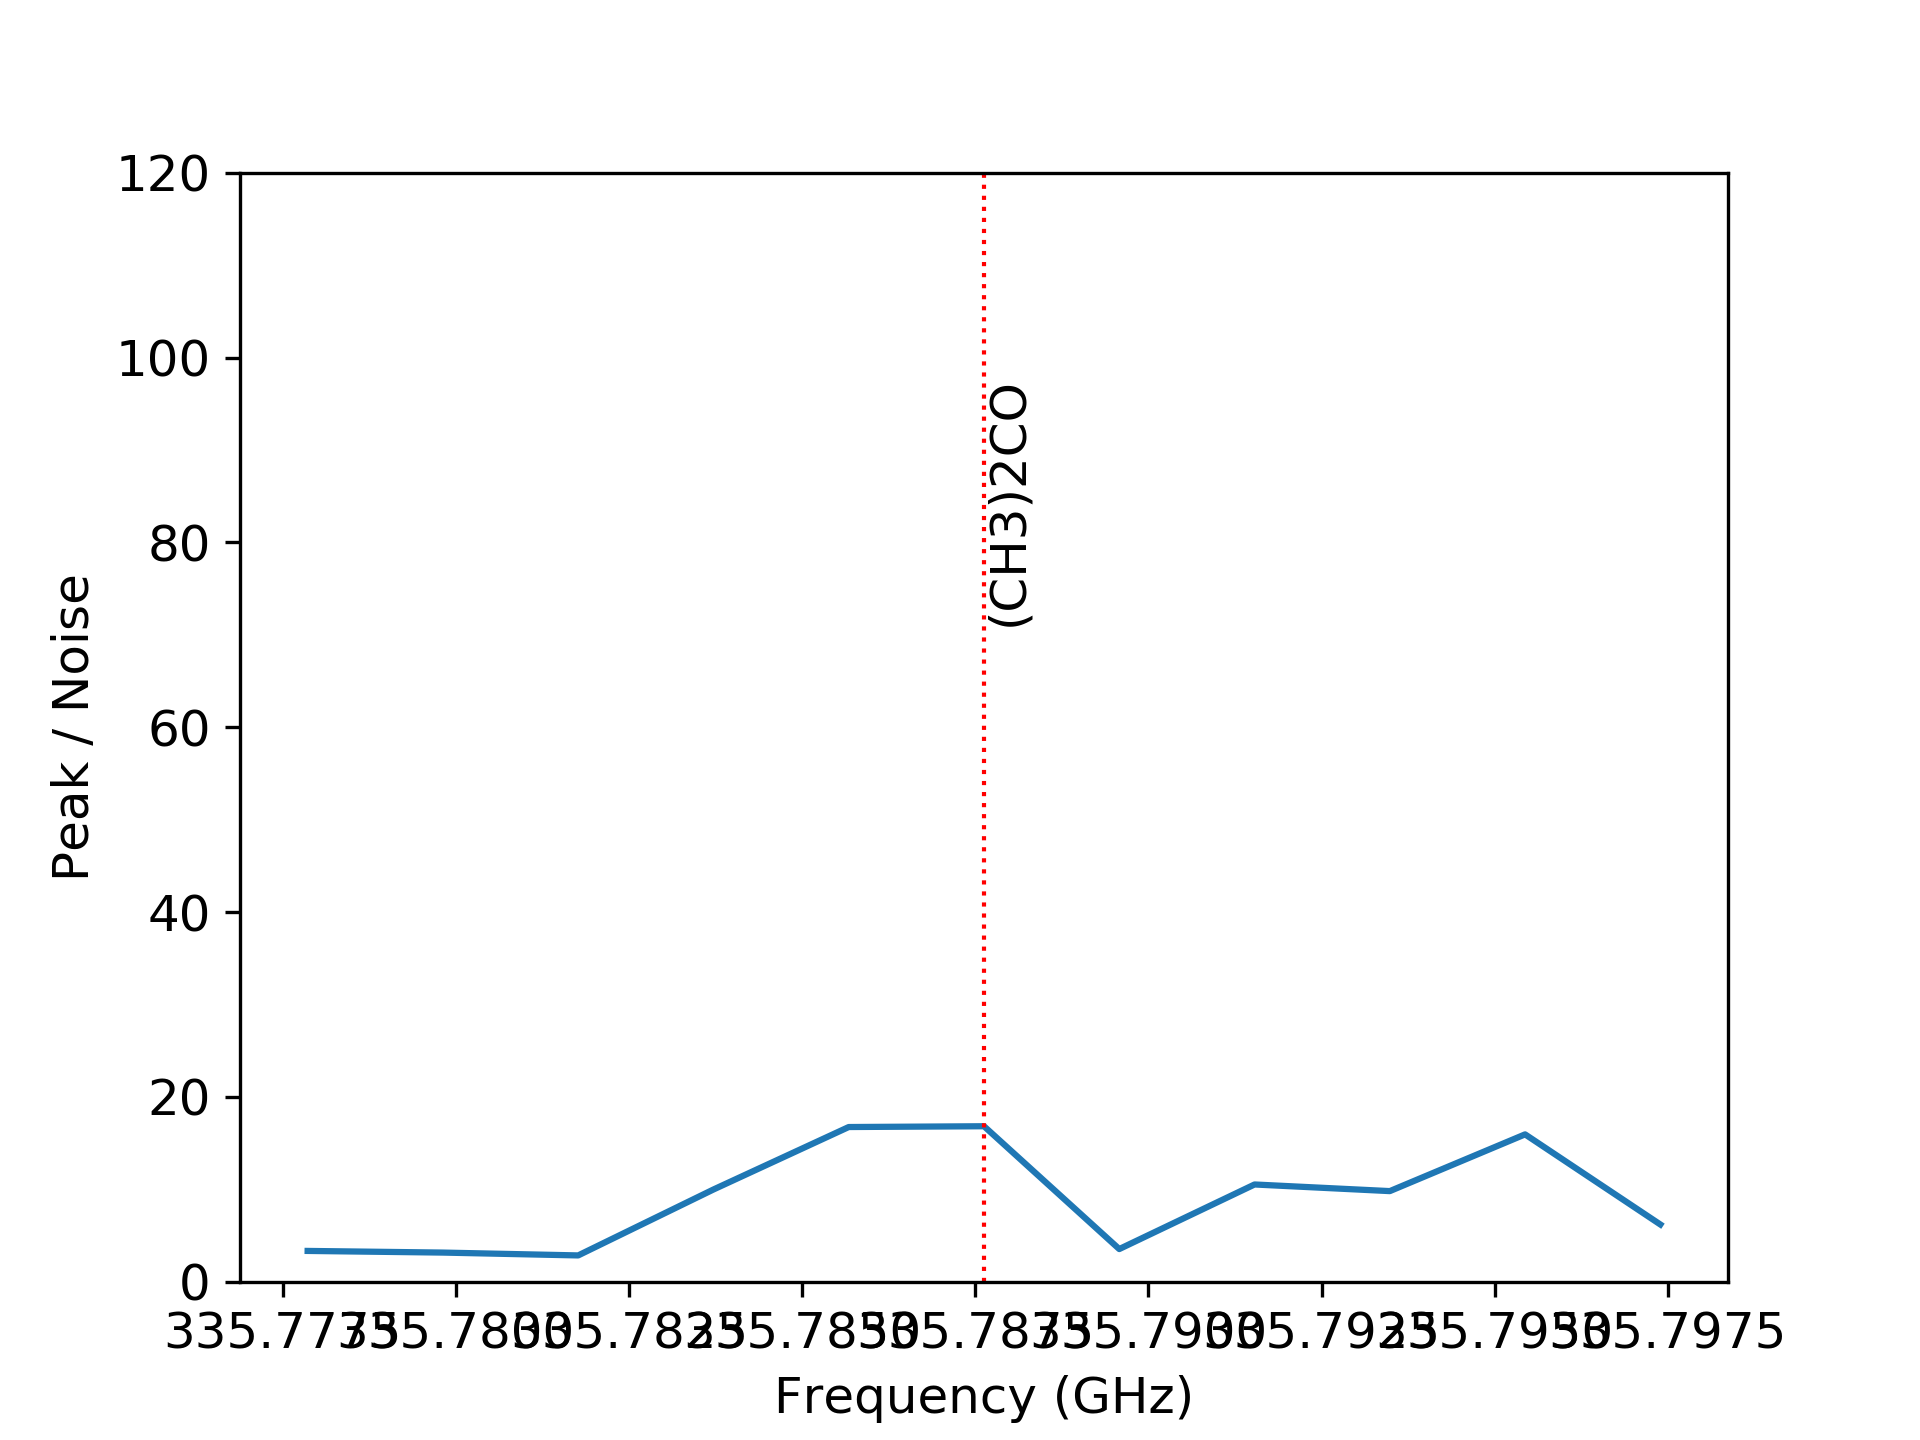
\includegraphics[width=0.33\textwidth]{spw2_(CH3)2CO}
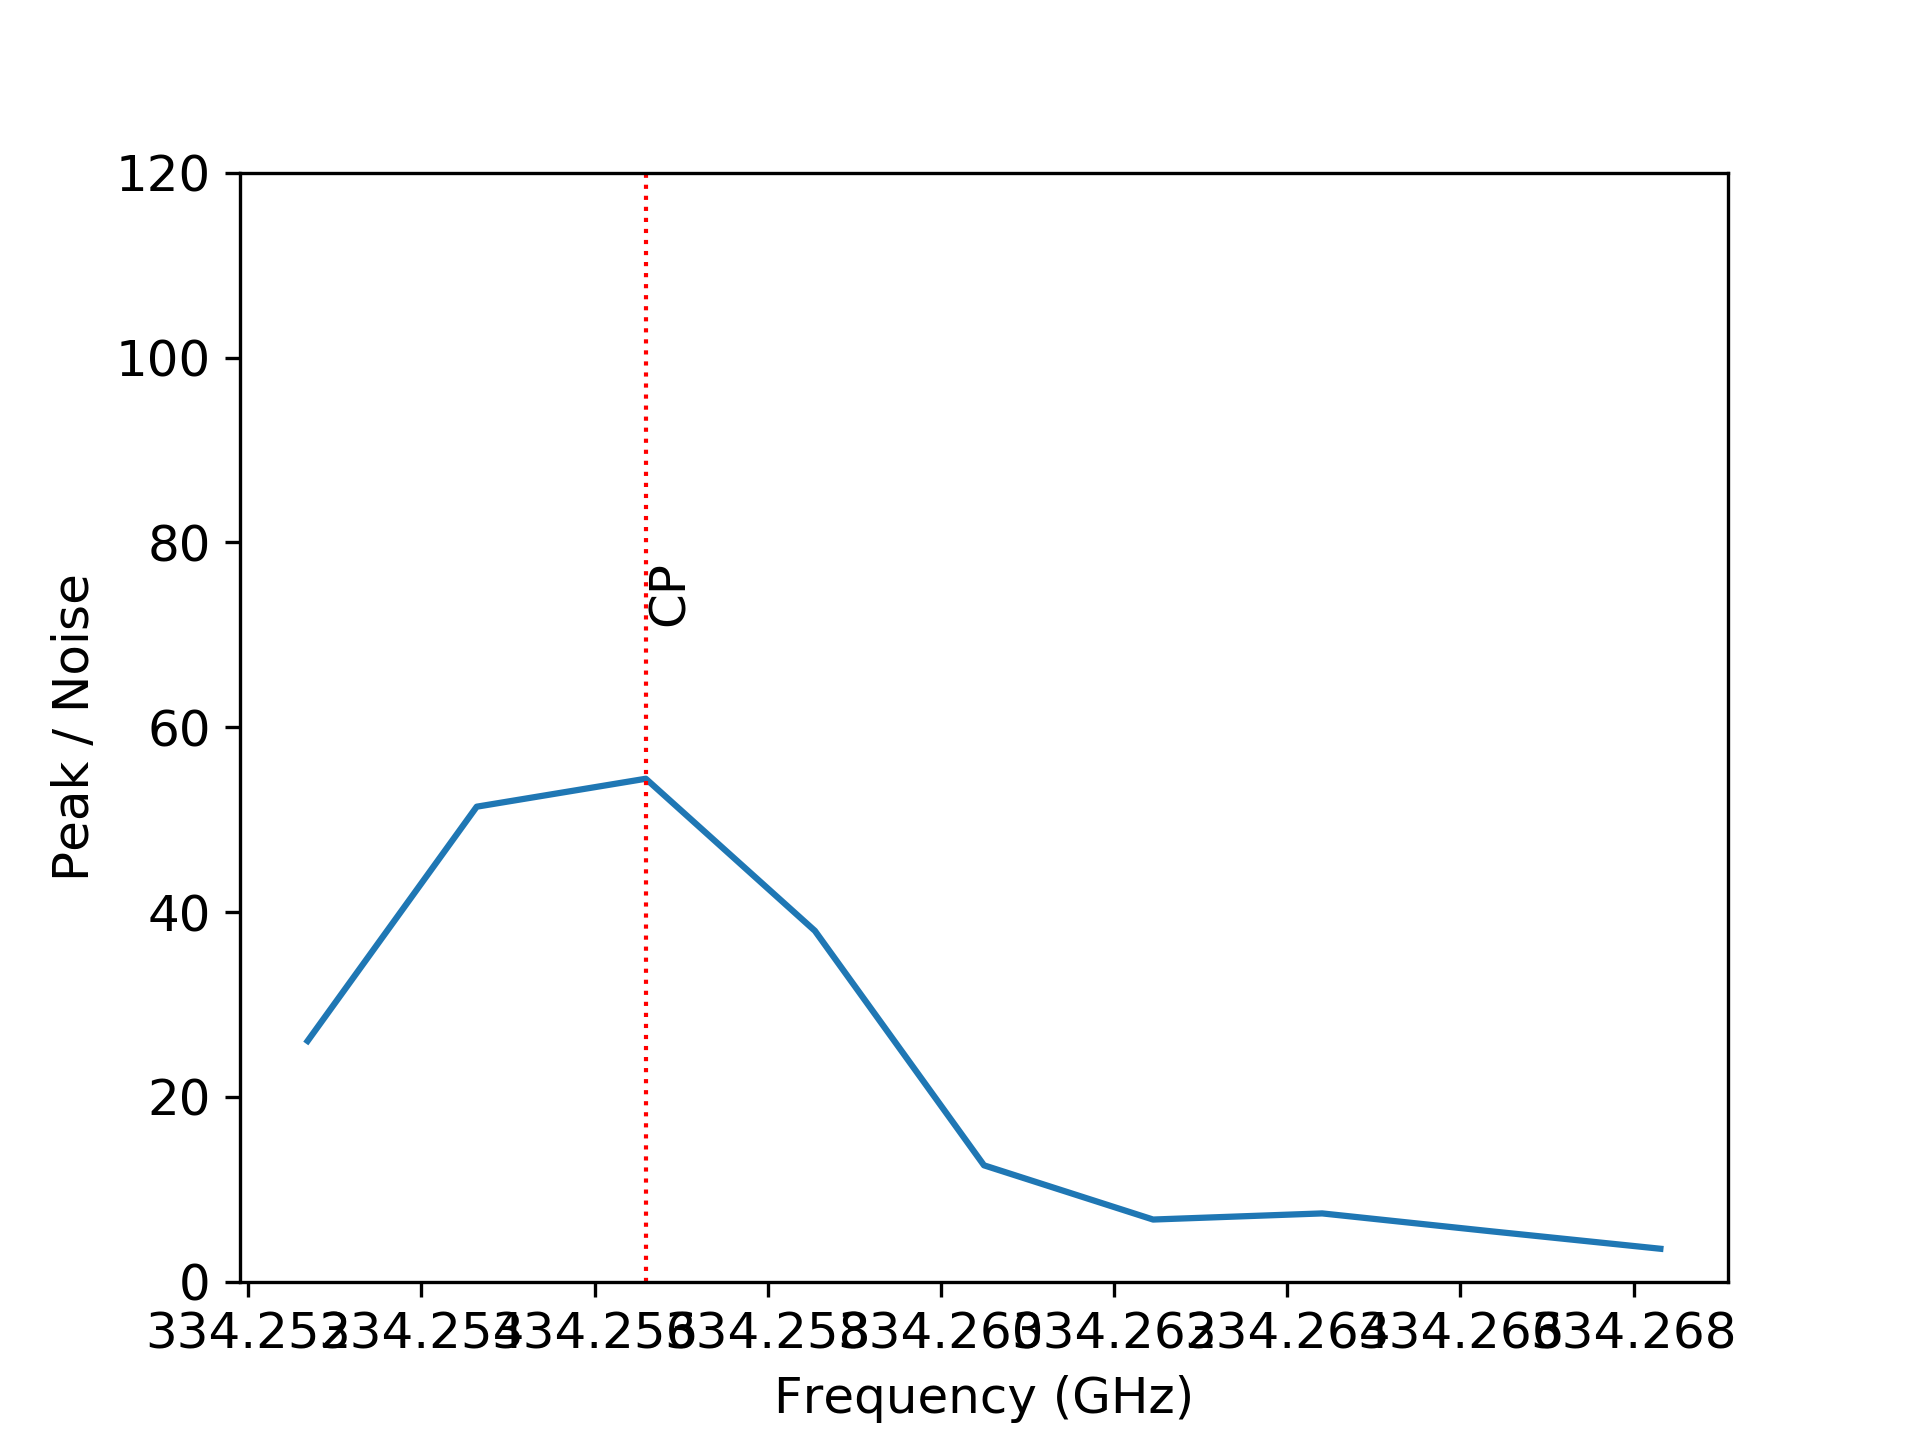
\includegraphics[width=0.33\textwidth]{spw2_CP}
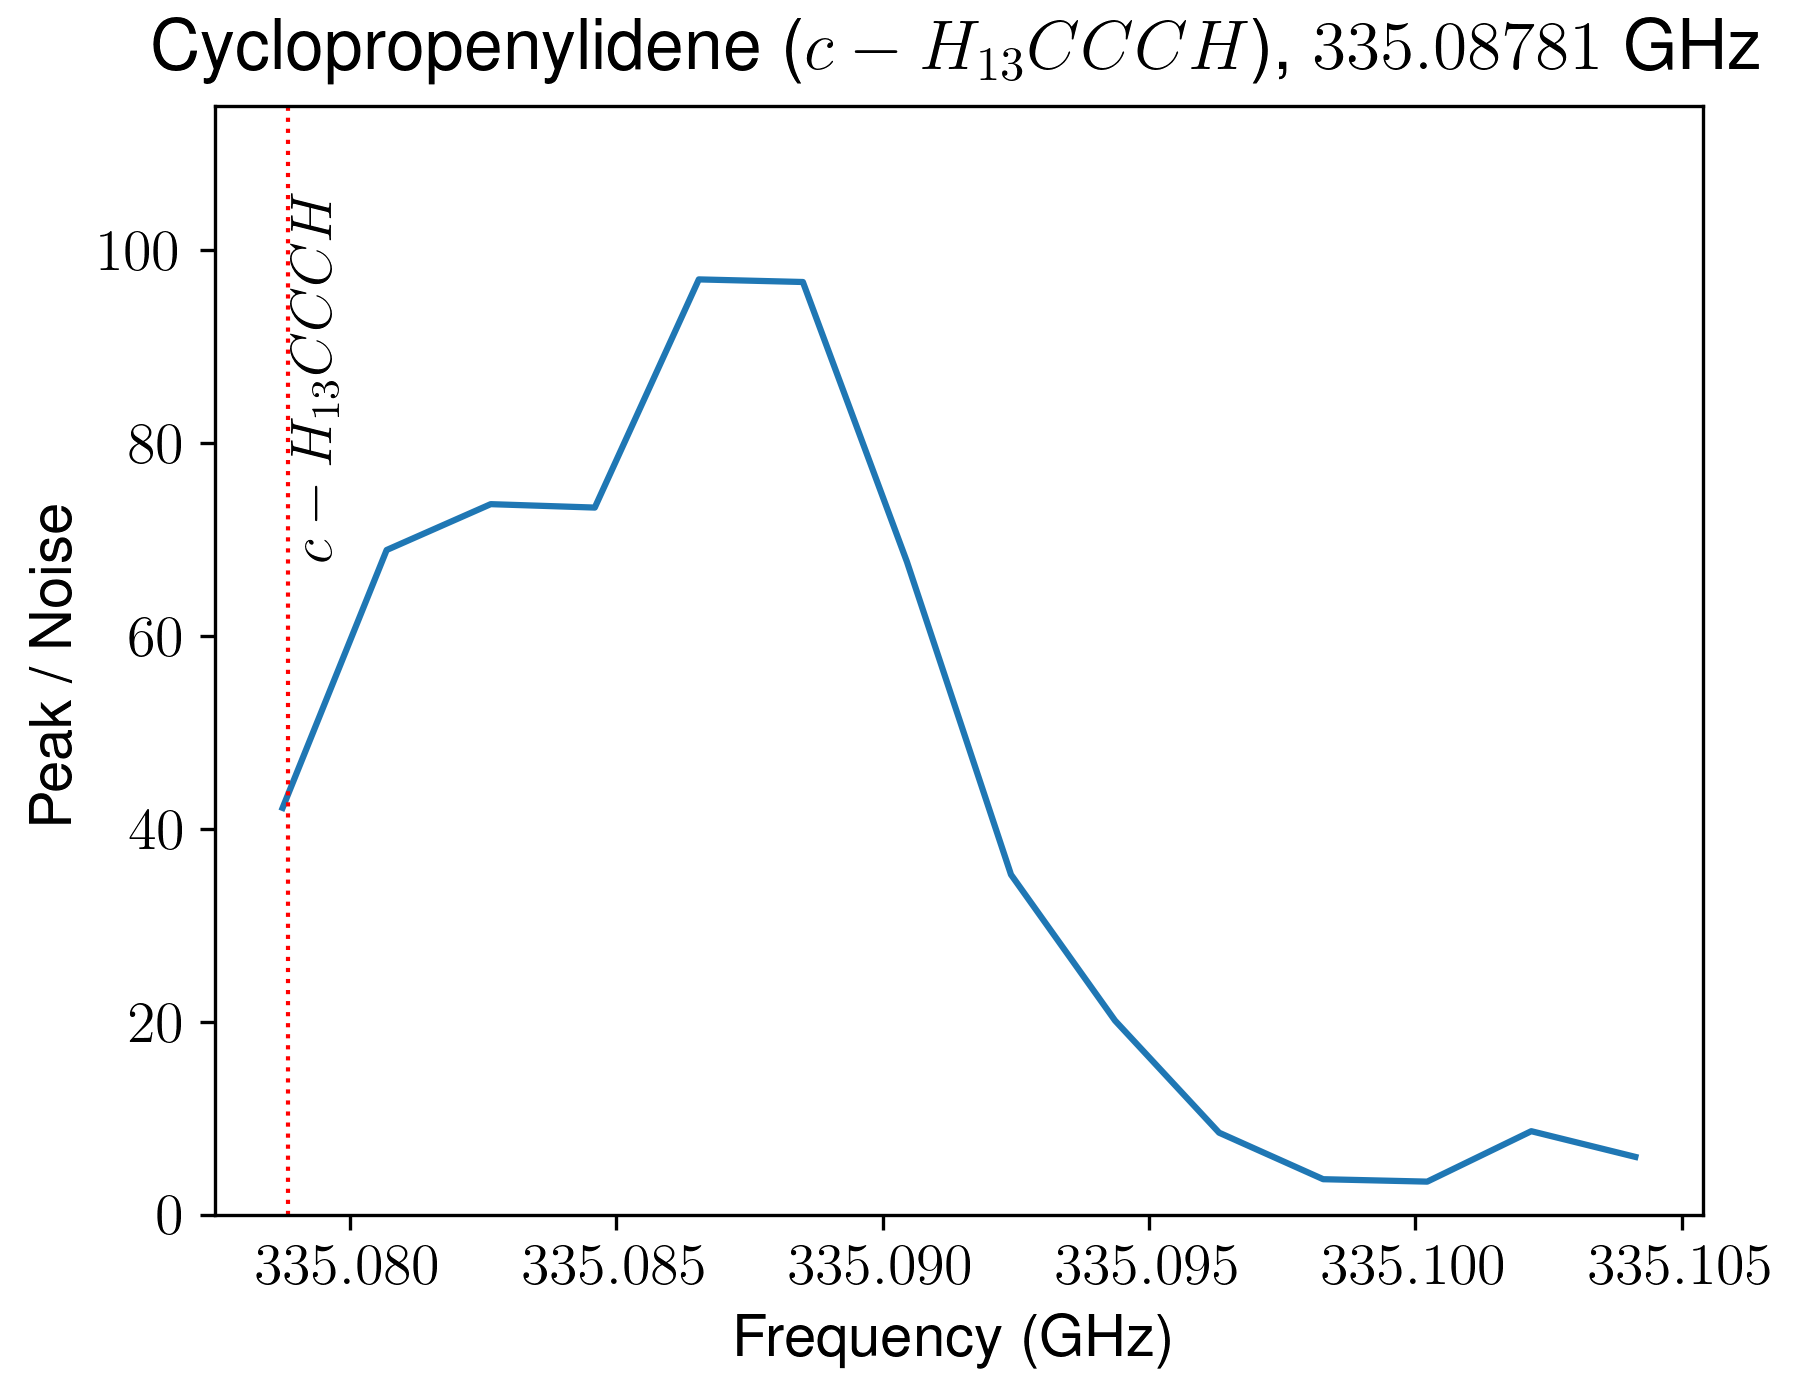
\includegraphics[width=0.33\textwidth]{spw2_c-H13CCCH}
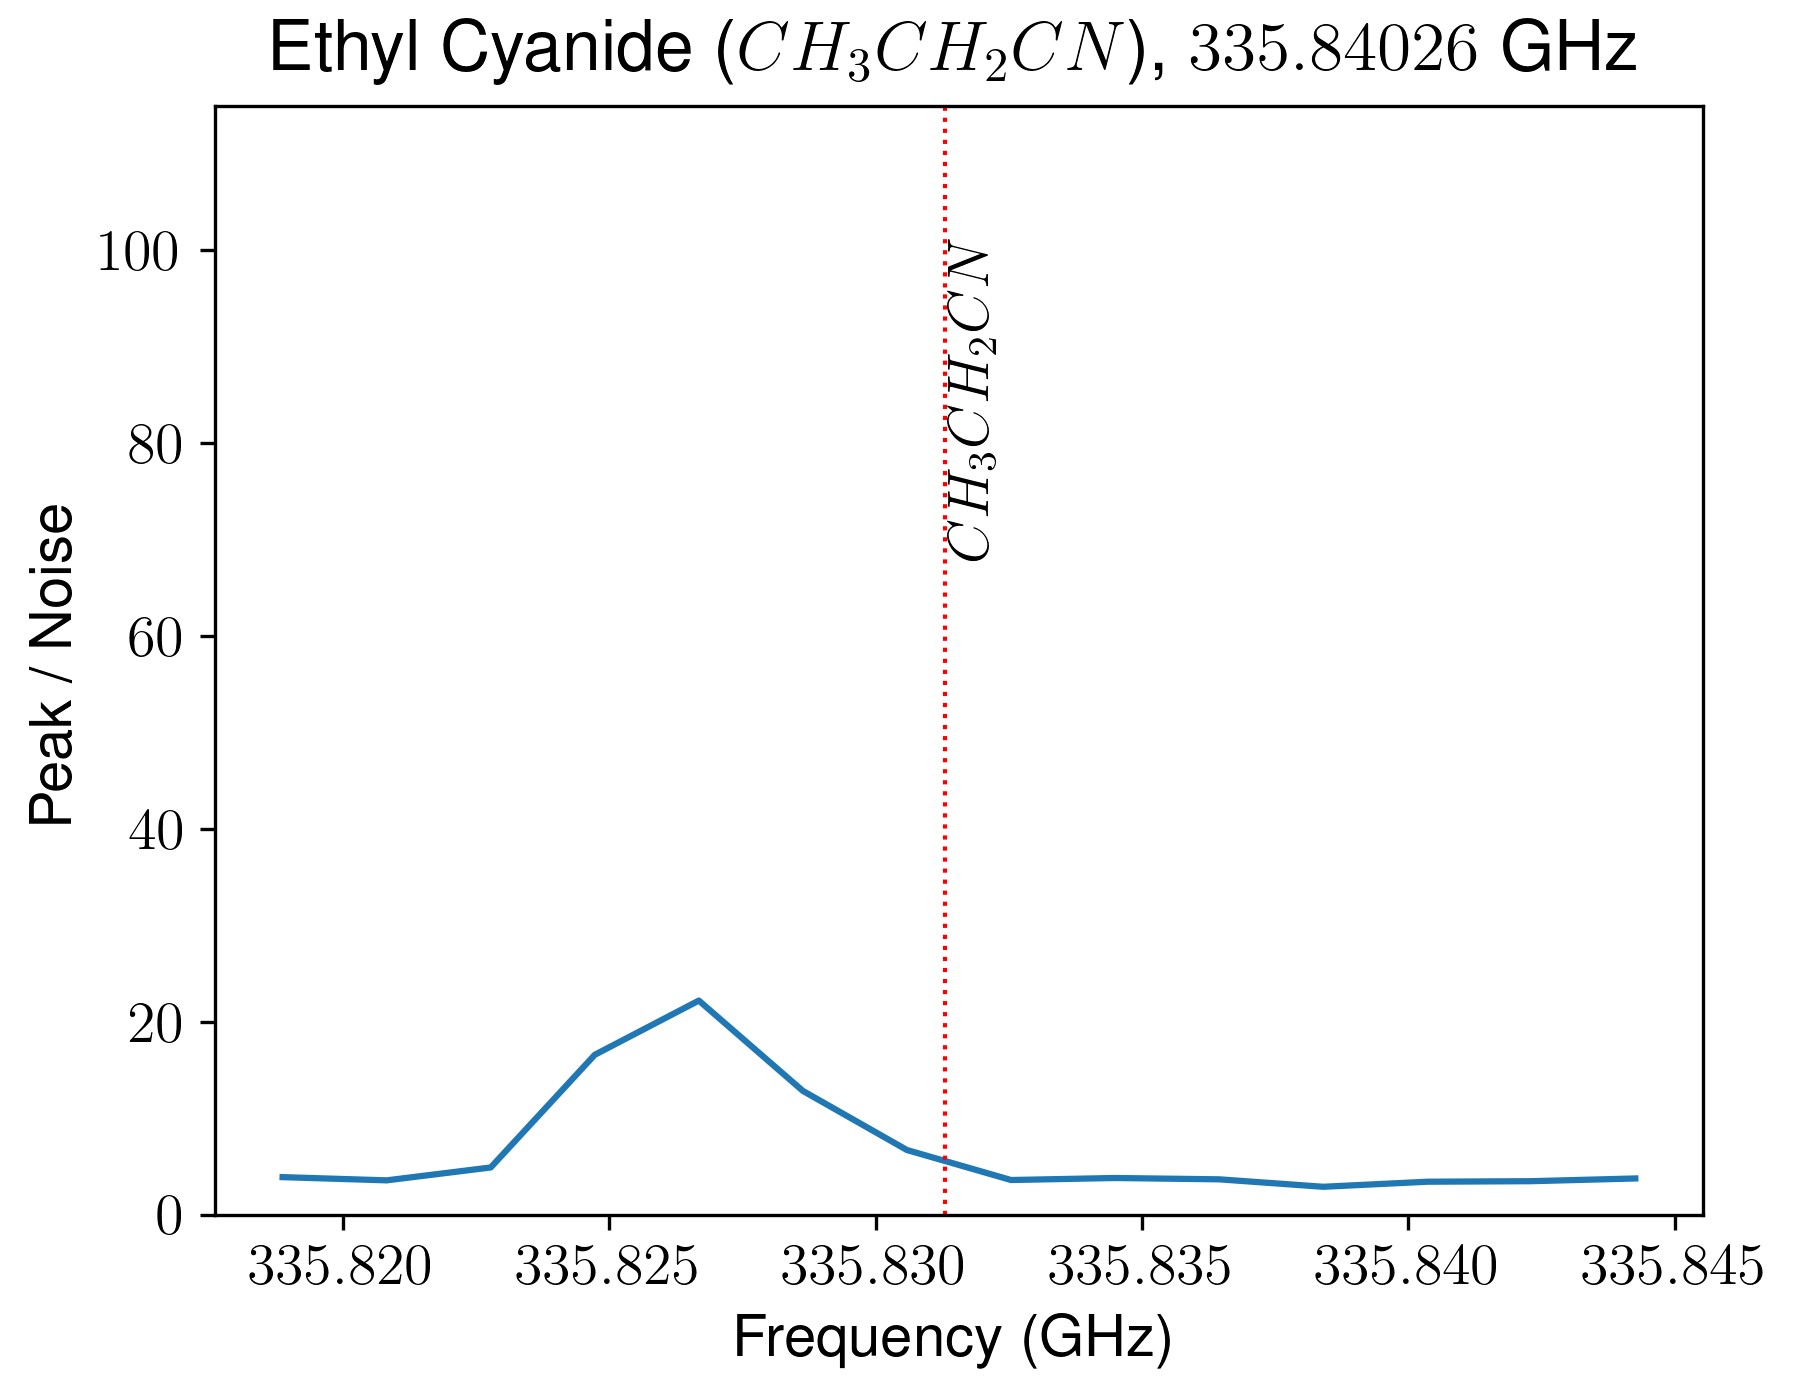
\includegraphics[width=0.33\textwidth]{spw2_CH3CH2CN}
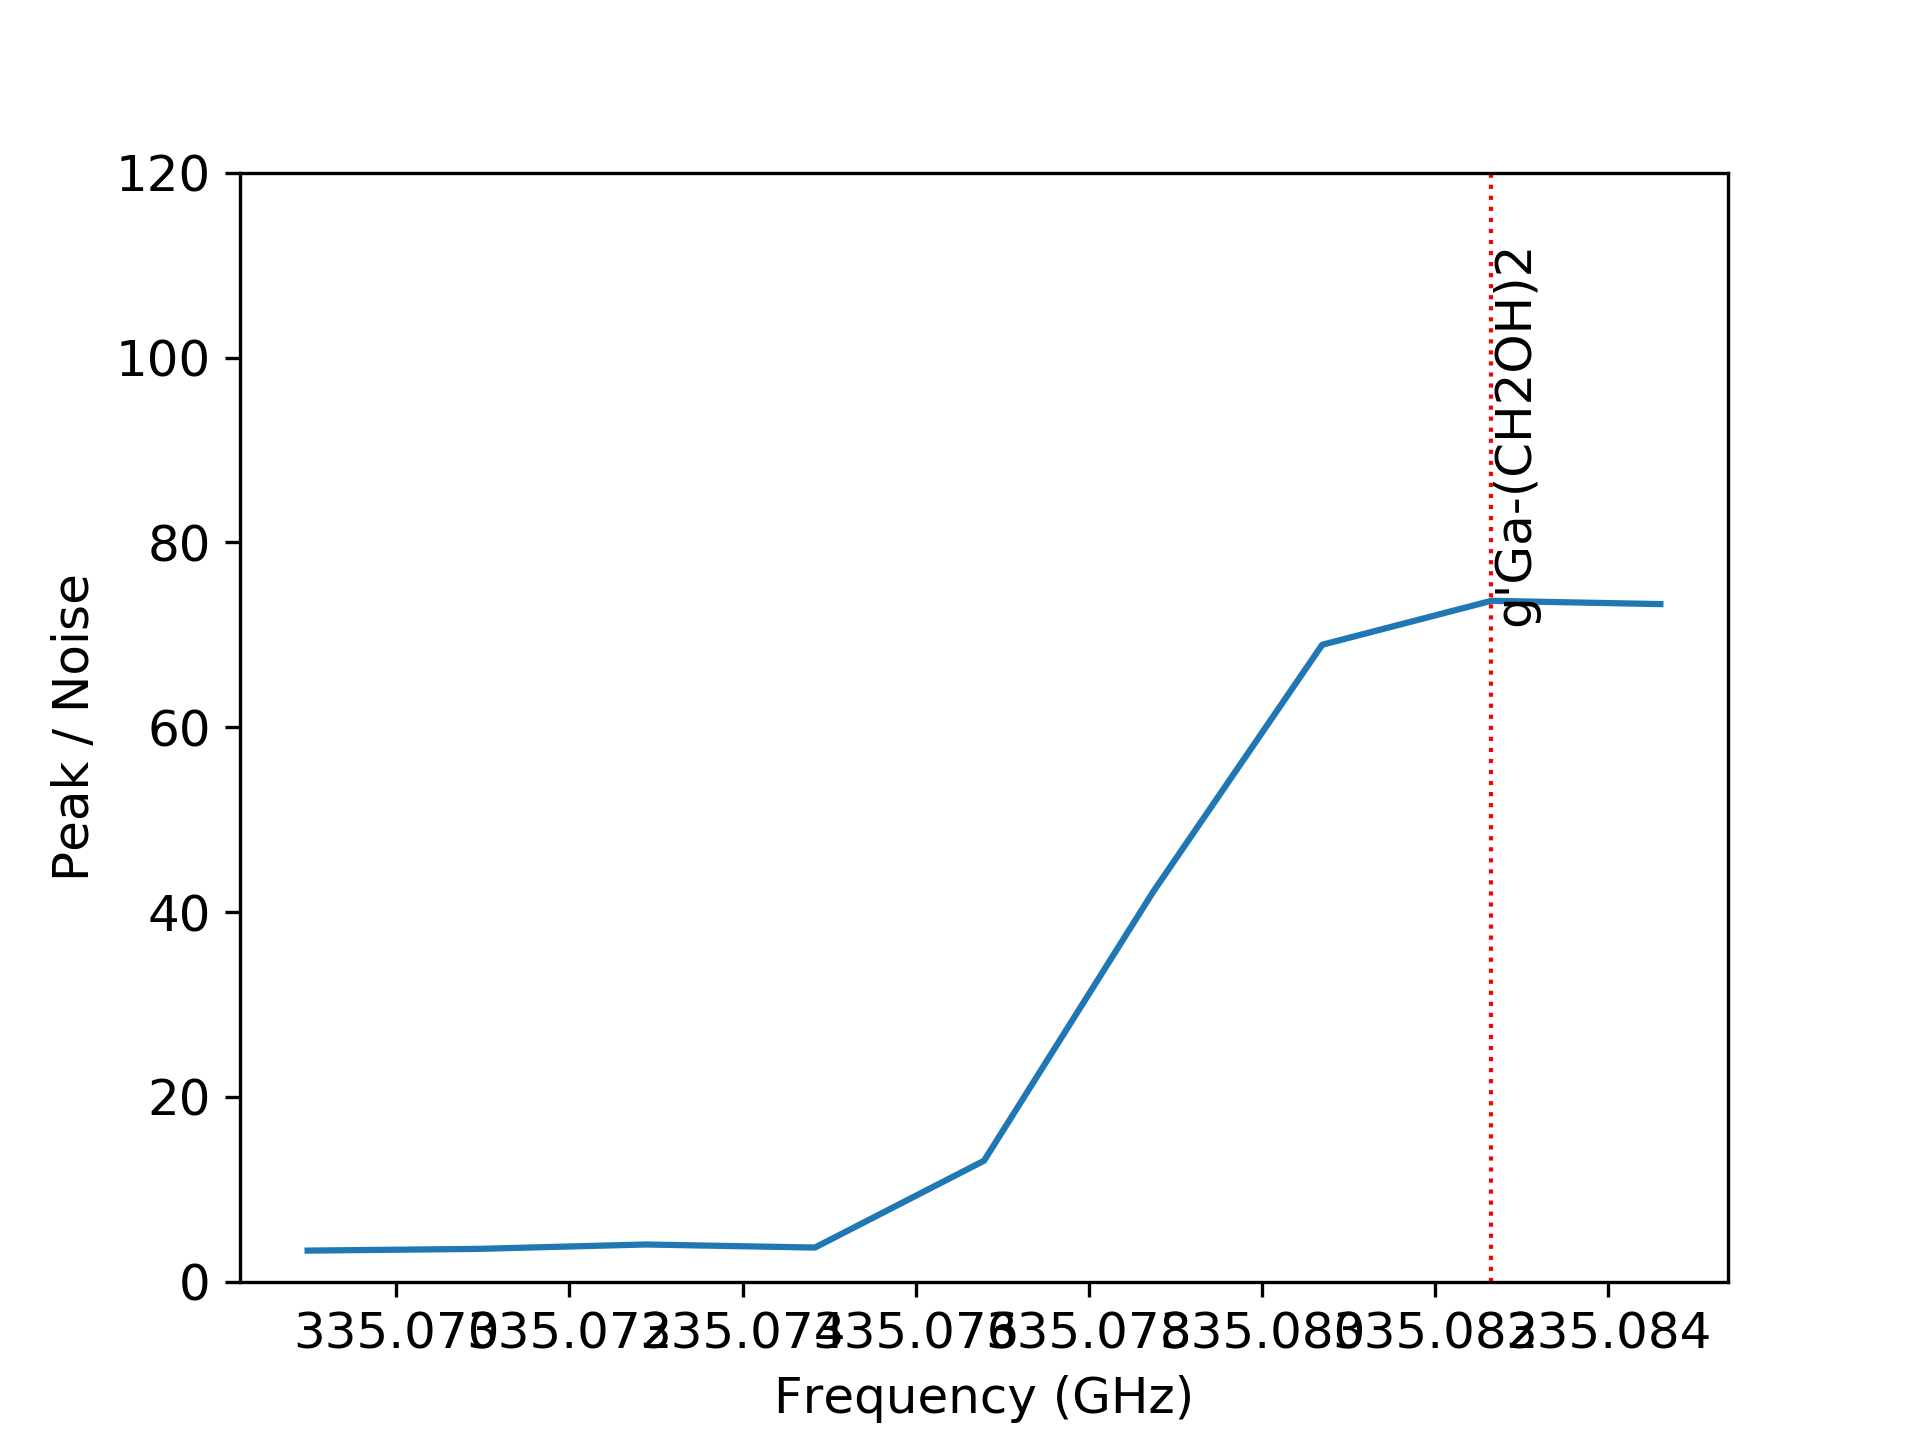
\includegraphics[width=0.33\textwidth]{spw2_g'Ga-(CH2OH)2}
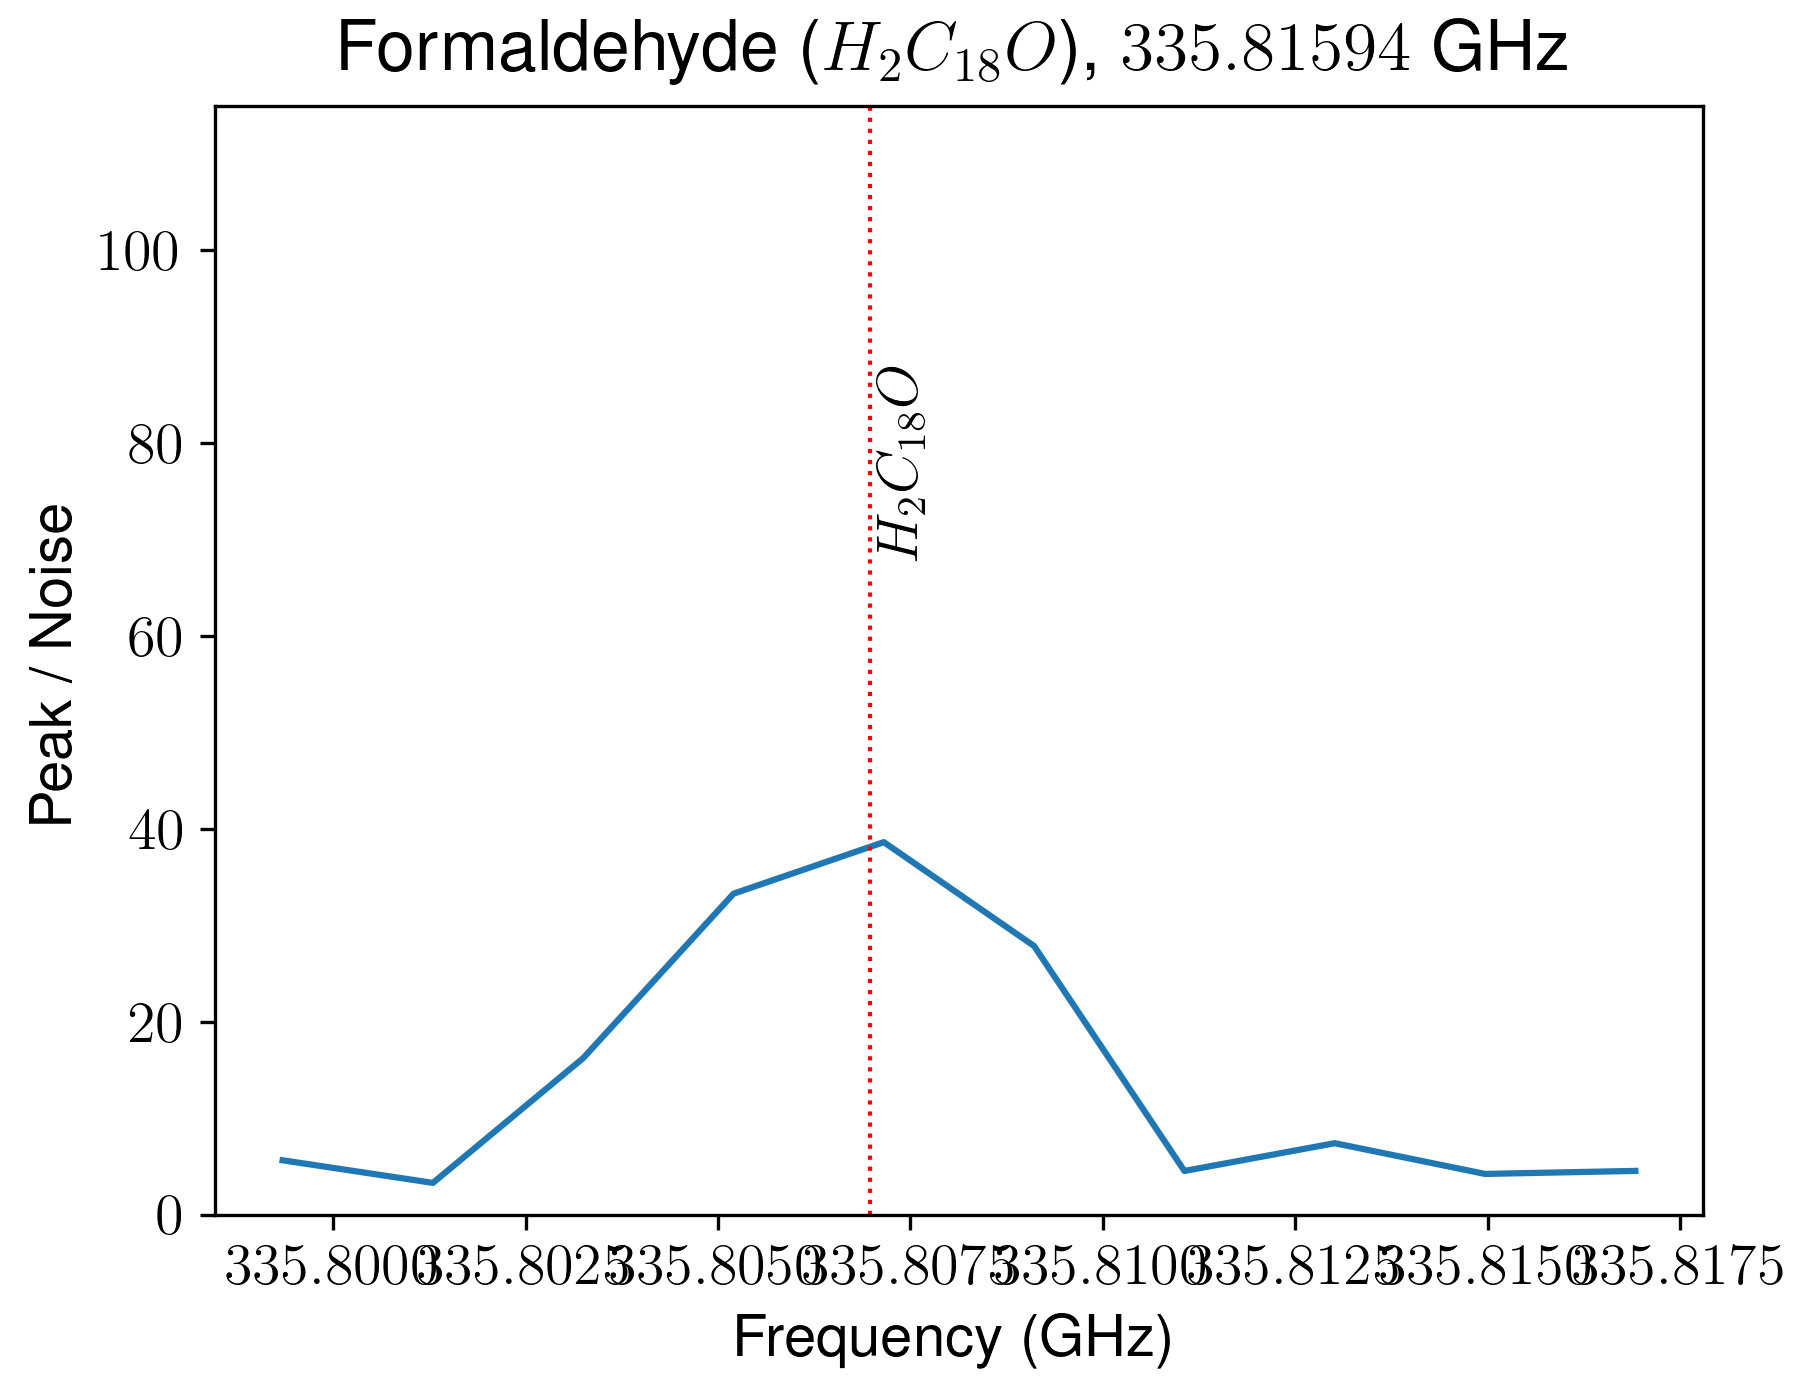
\includegraphics[width=0.33\textwidth]{spw2_H2C18O}
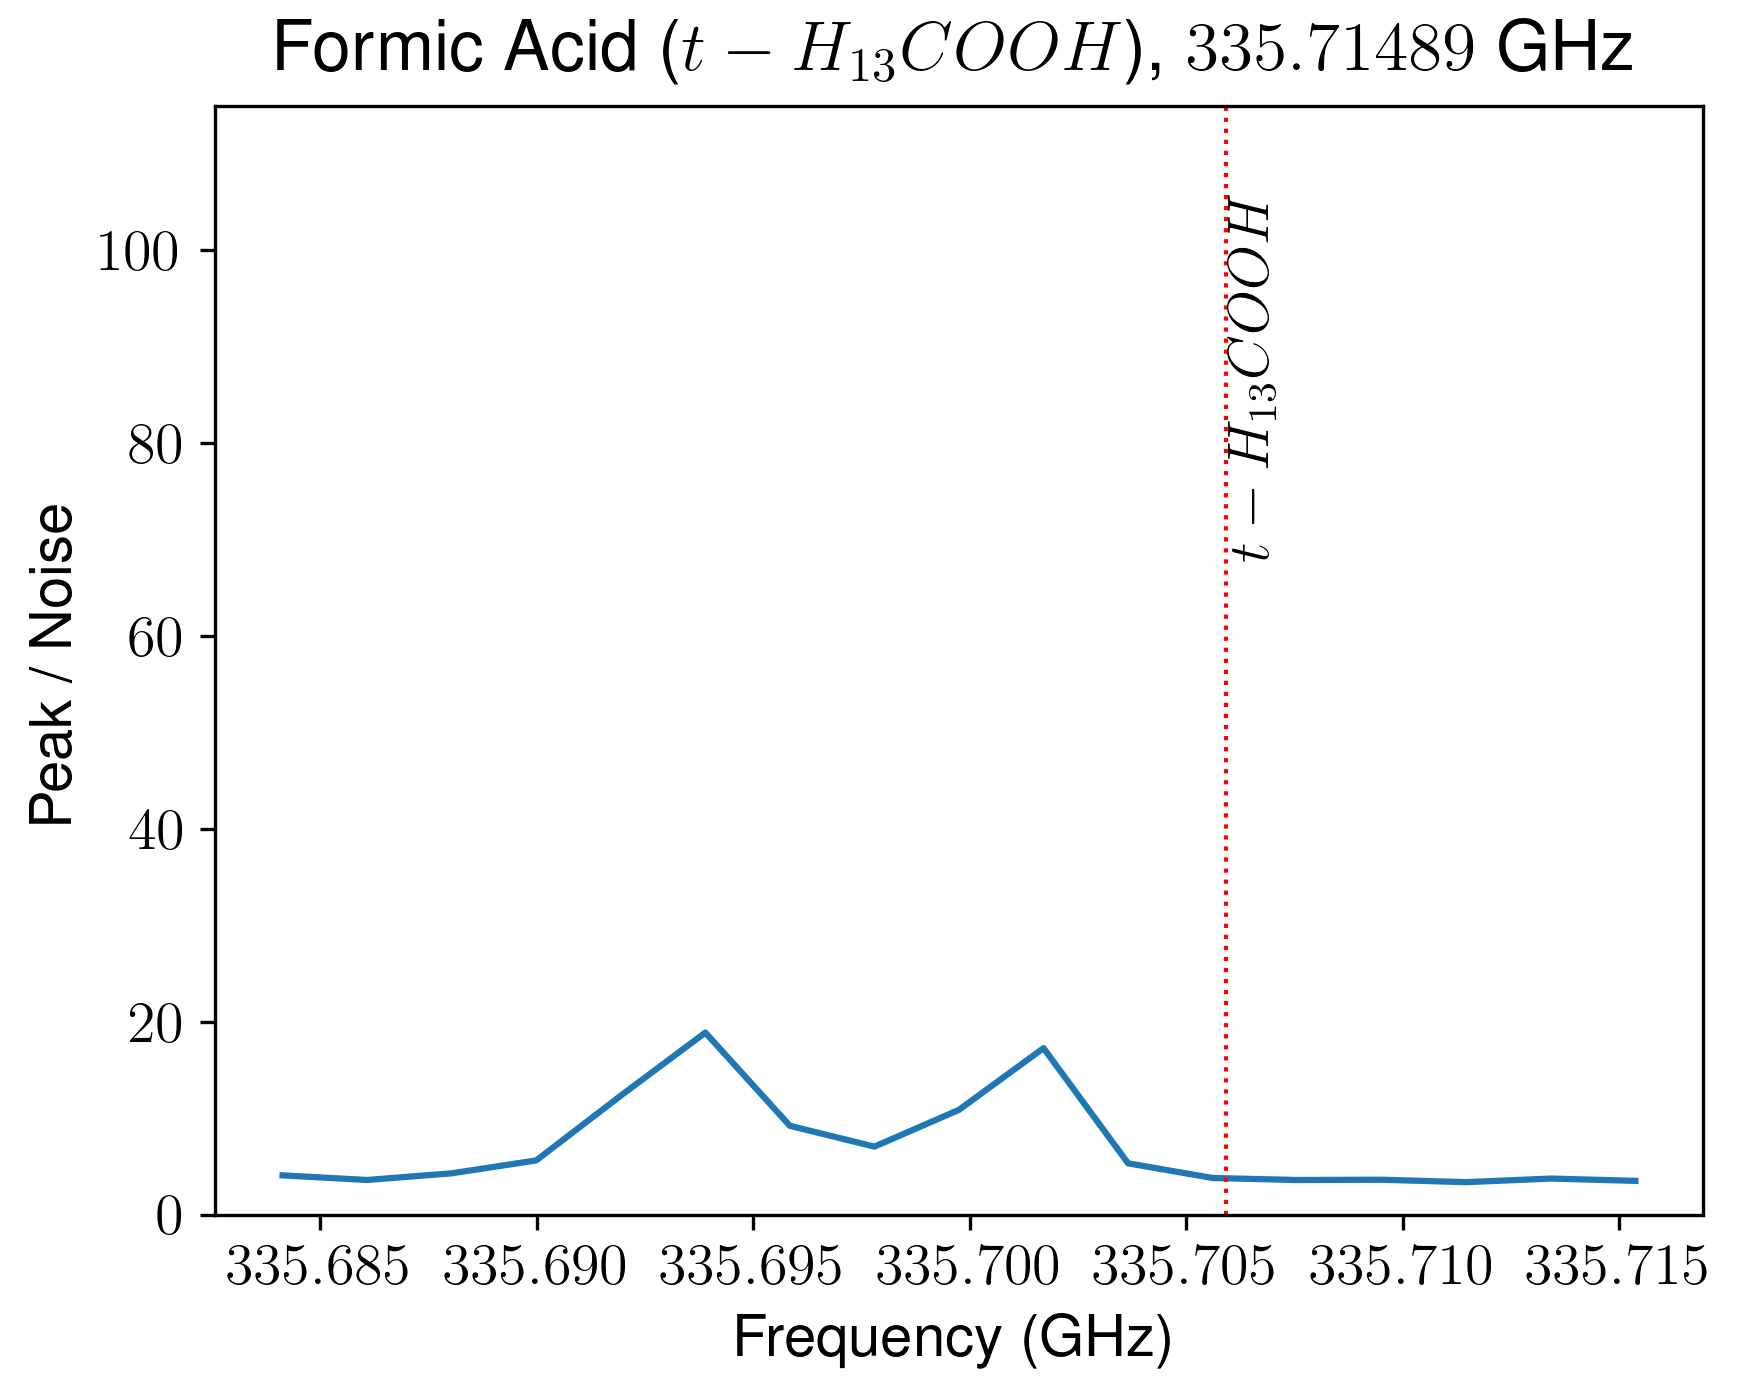
\includegraphics[width=0.33\textwidth]{spw2_t-H13COOH}
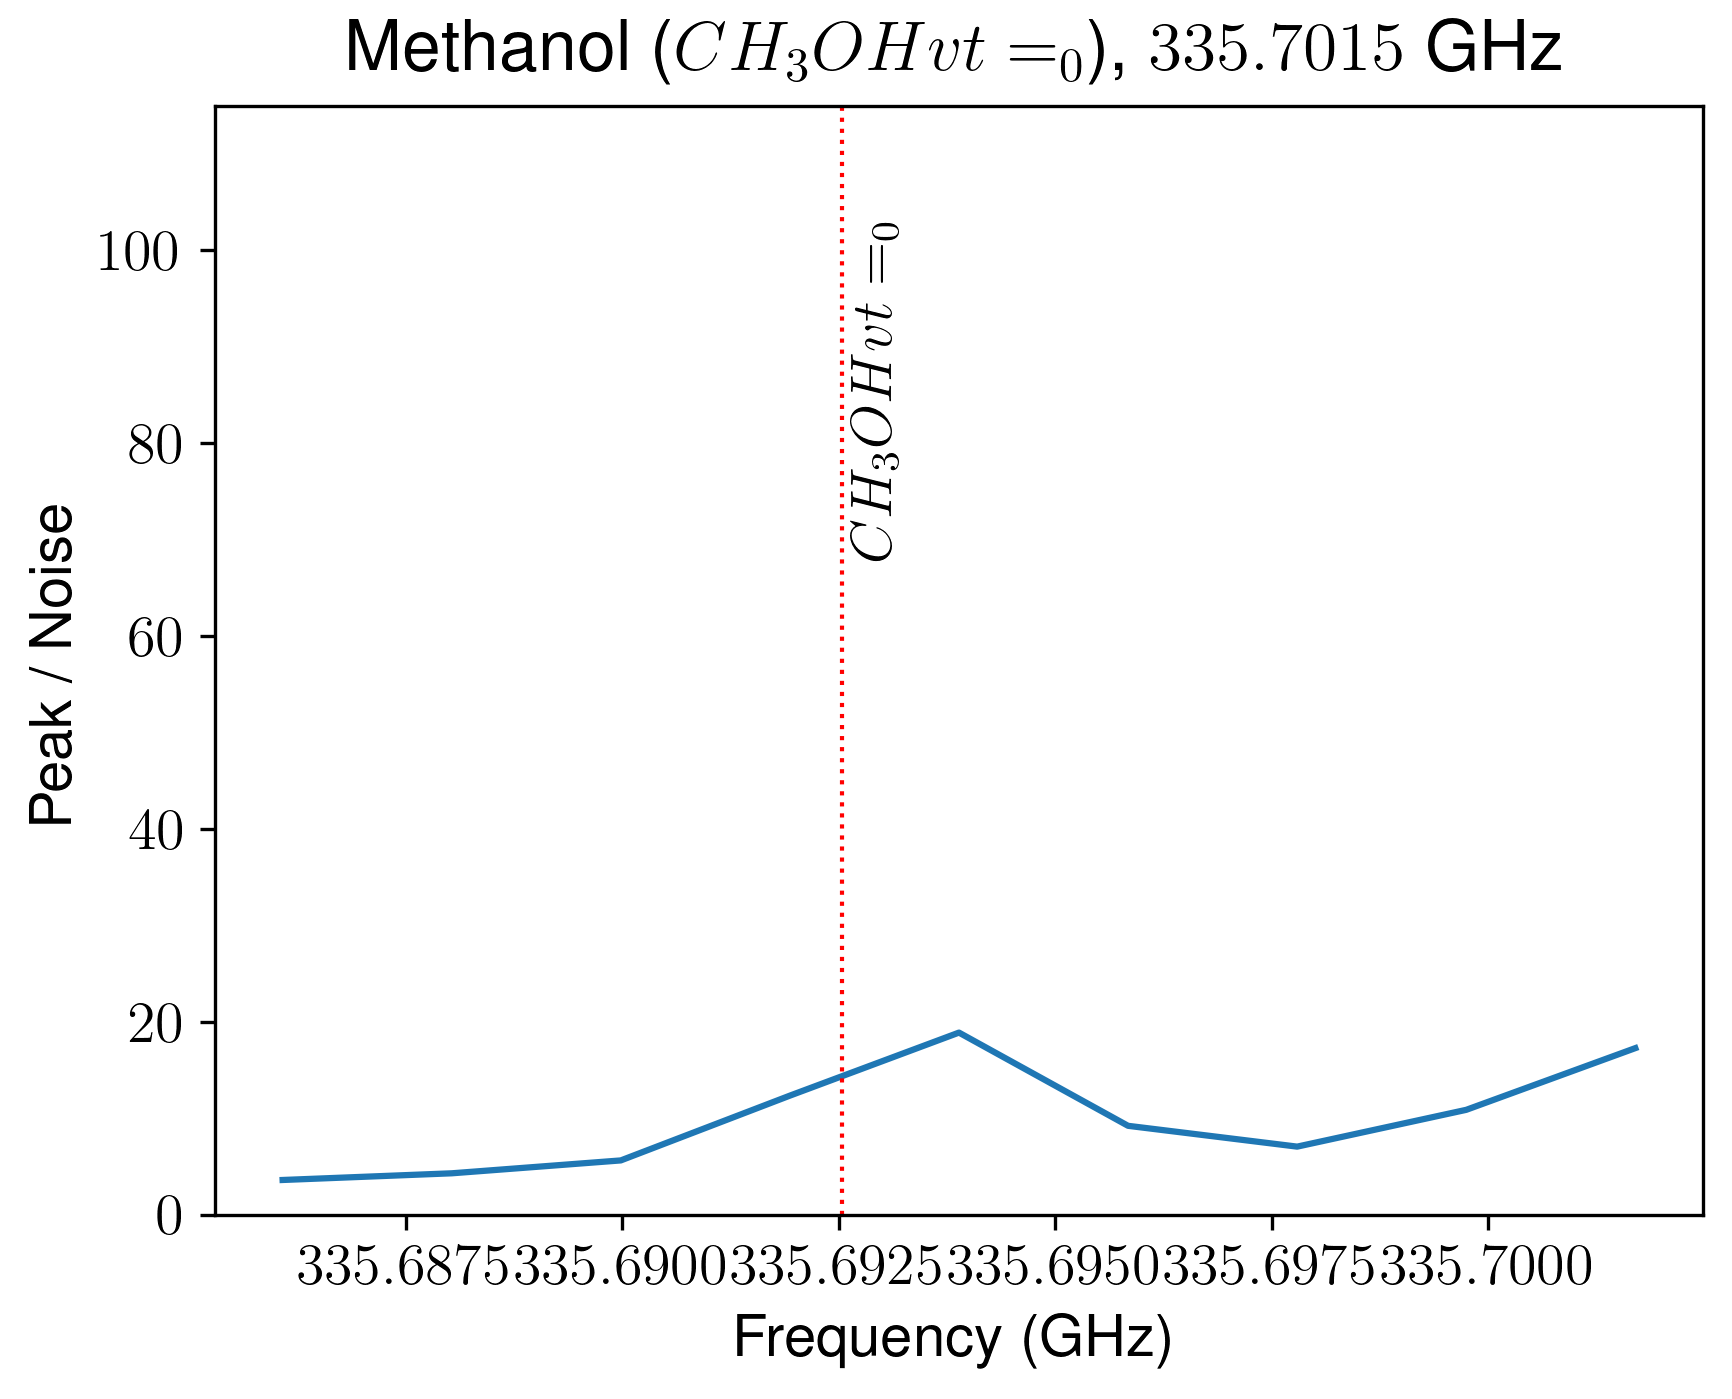
\includegraphics[width=0.33\textwidth]{spw2_CH3OHvt=0}
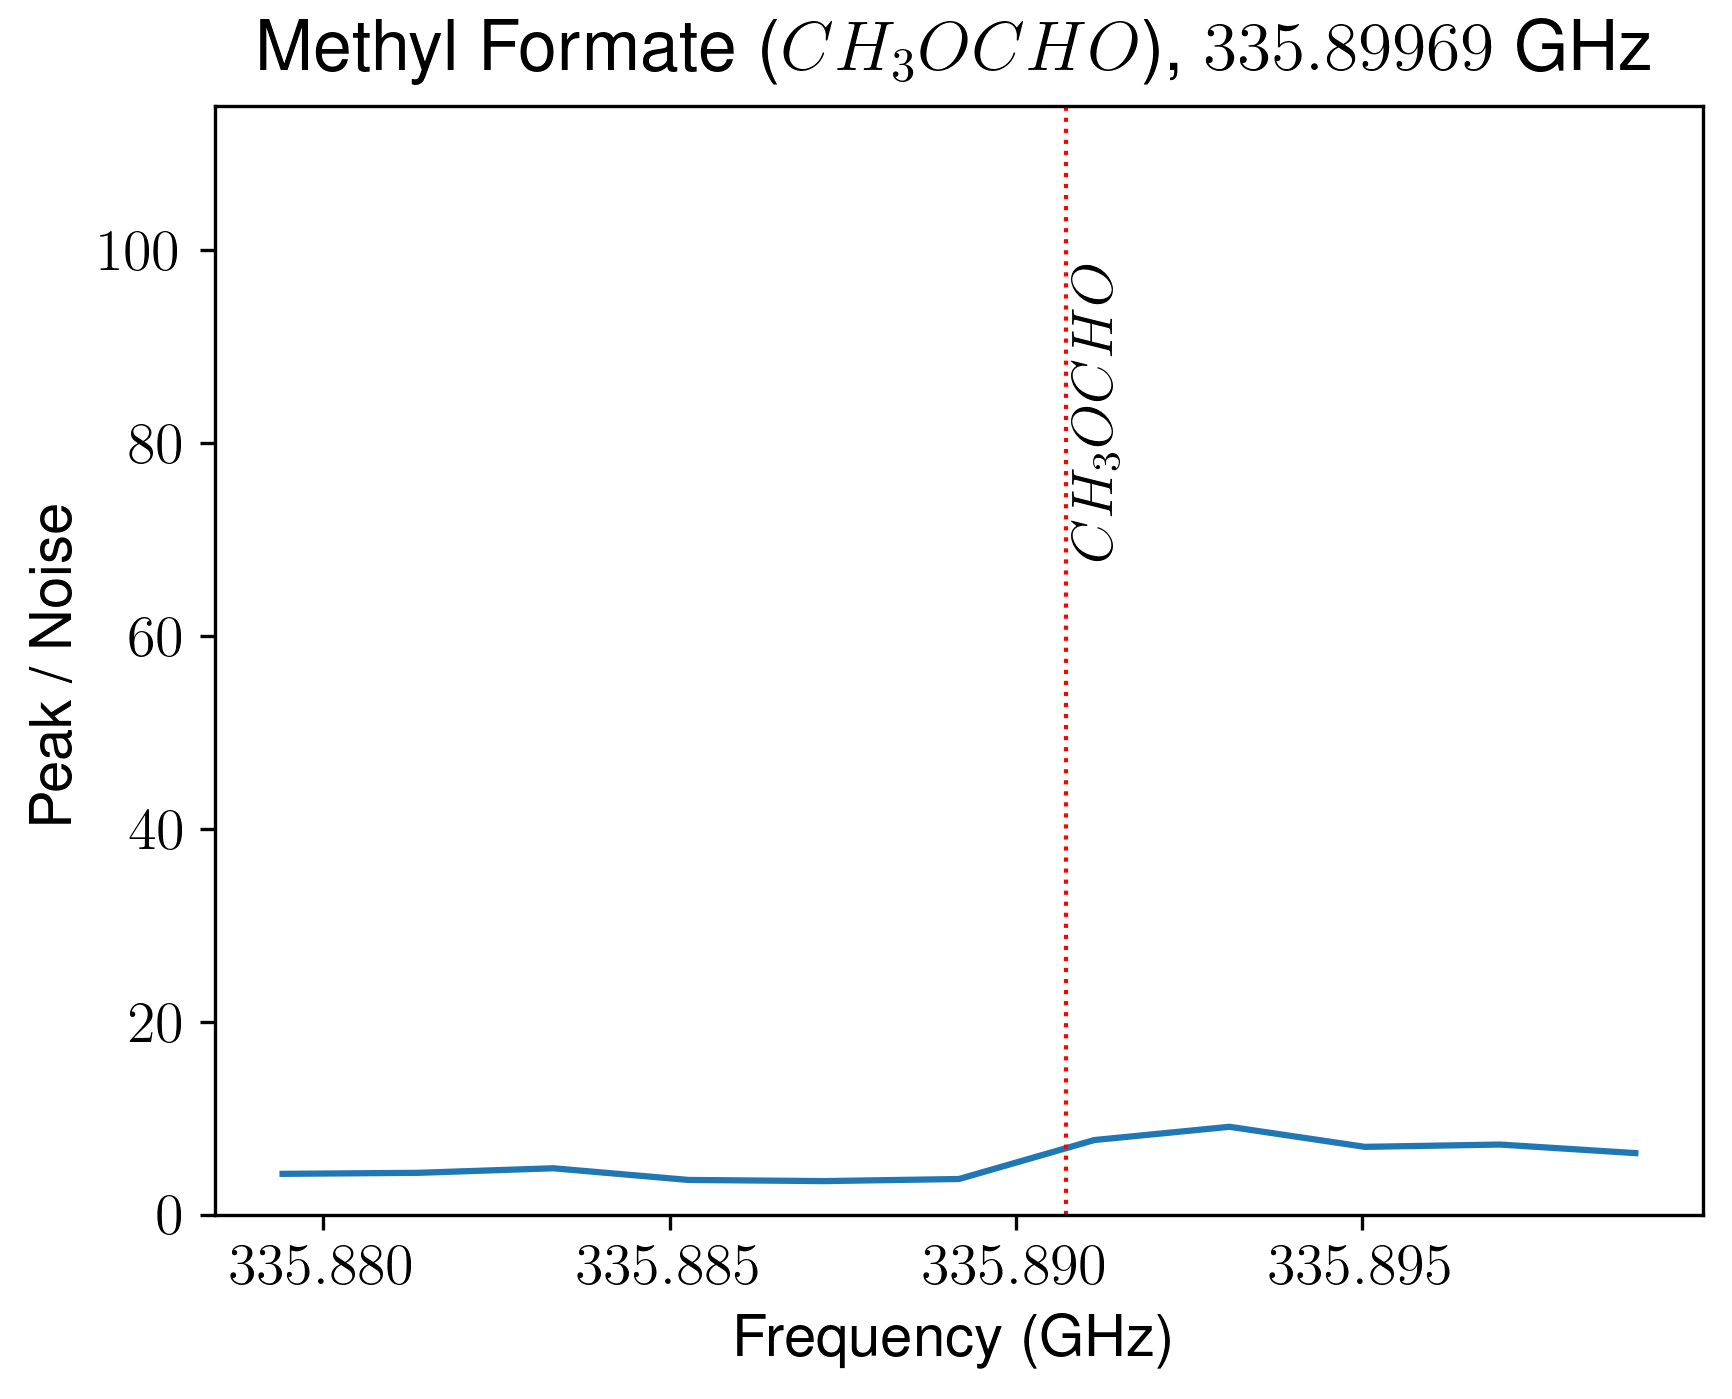
\includegraphics[width=0.33\textwidth]{spw2_CH3OCHO}
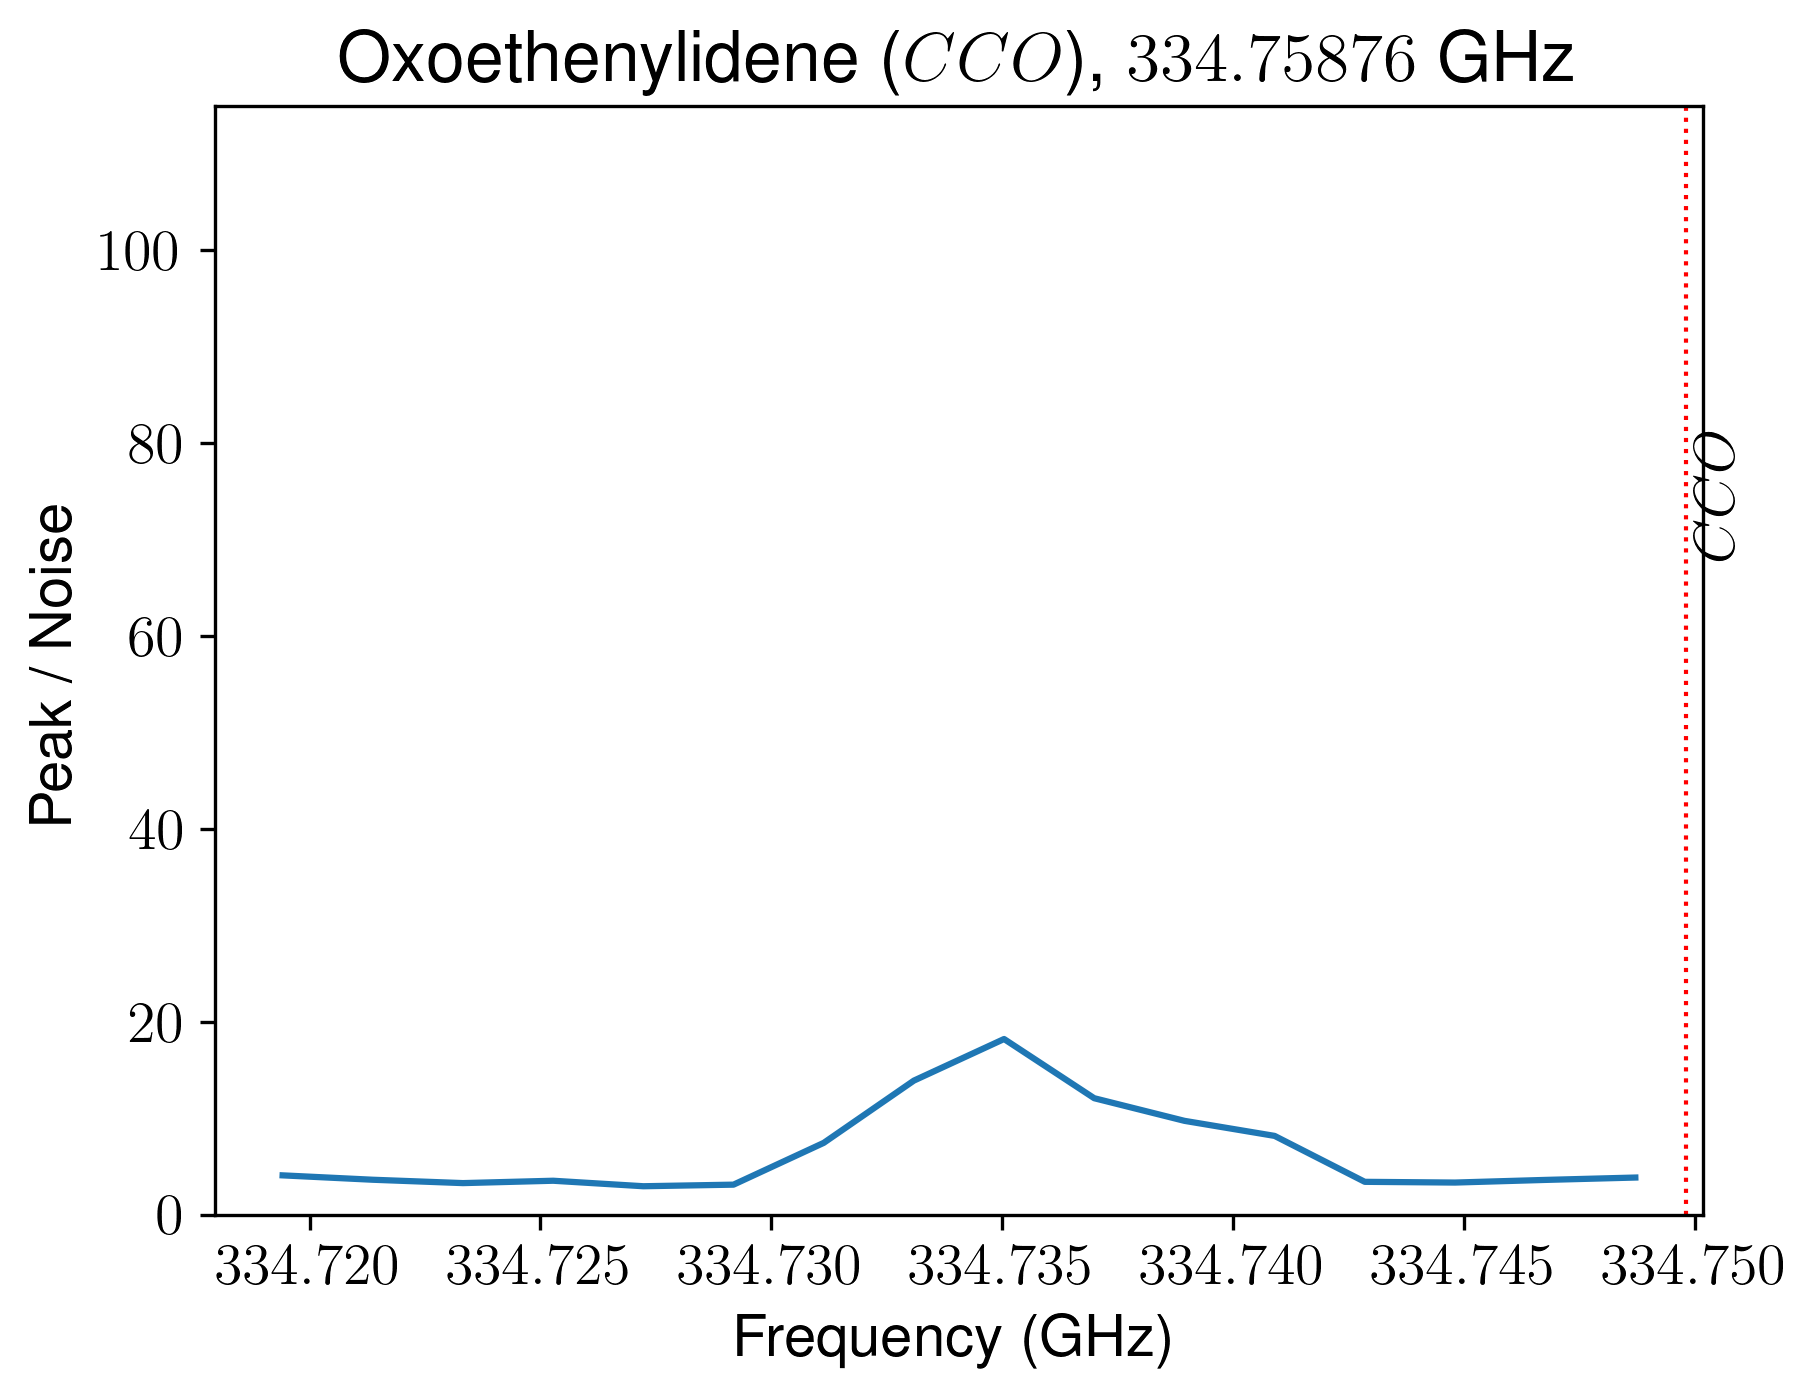
\includegraphics[width=0.33\textwidth]{spw2_CCO}
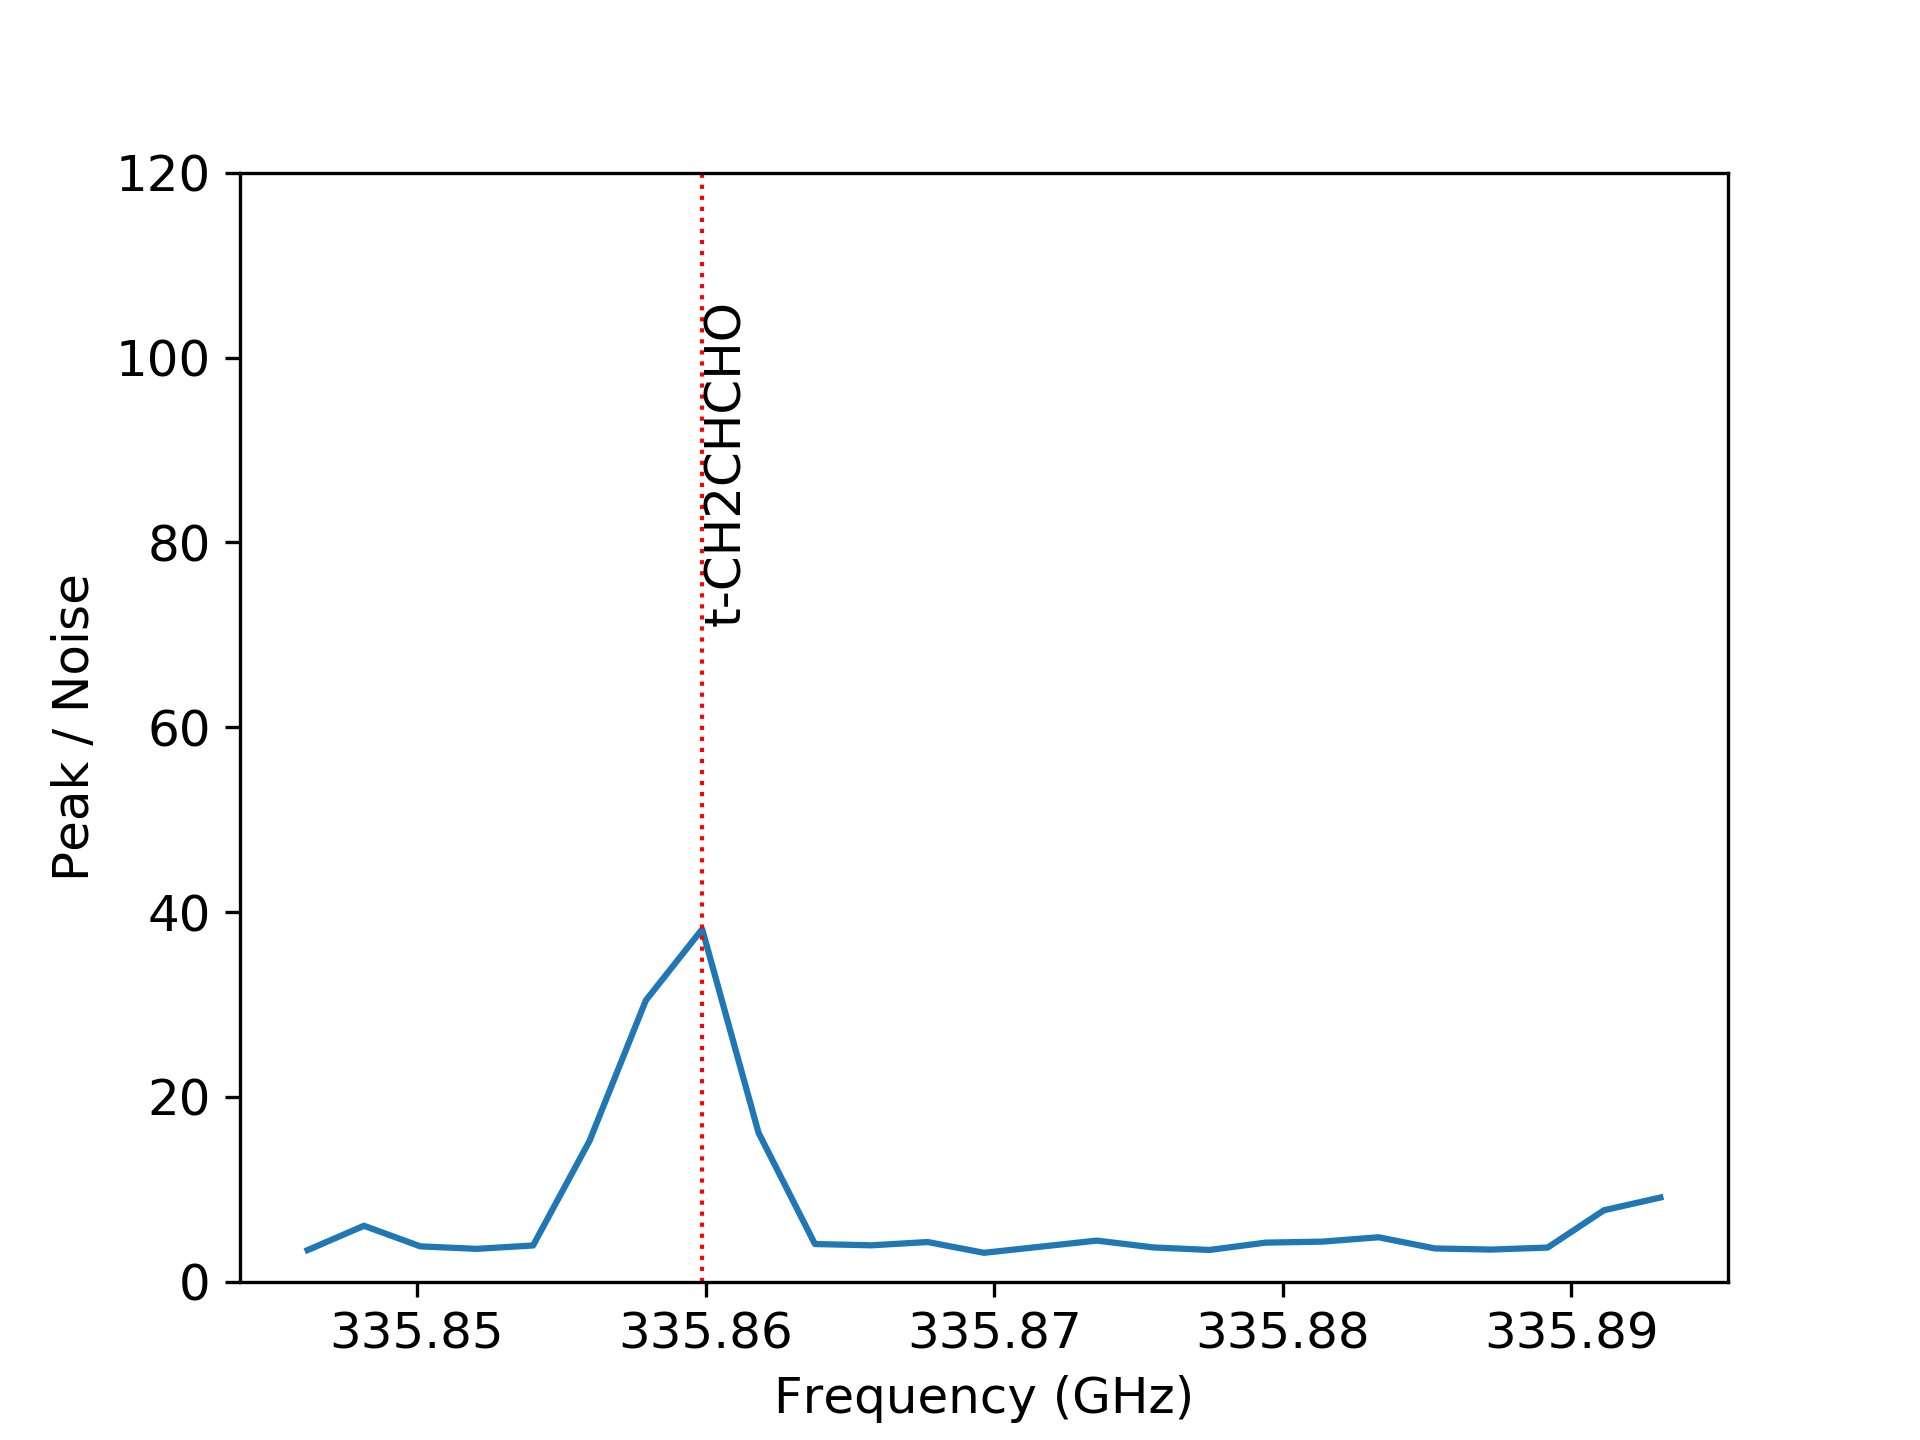
\includegraphics[width=0.33\textwidth]{spw2_t-CH2CHCHO}
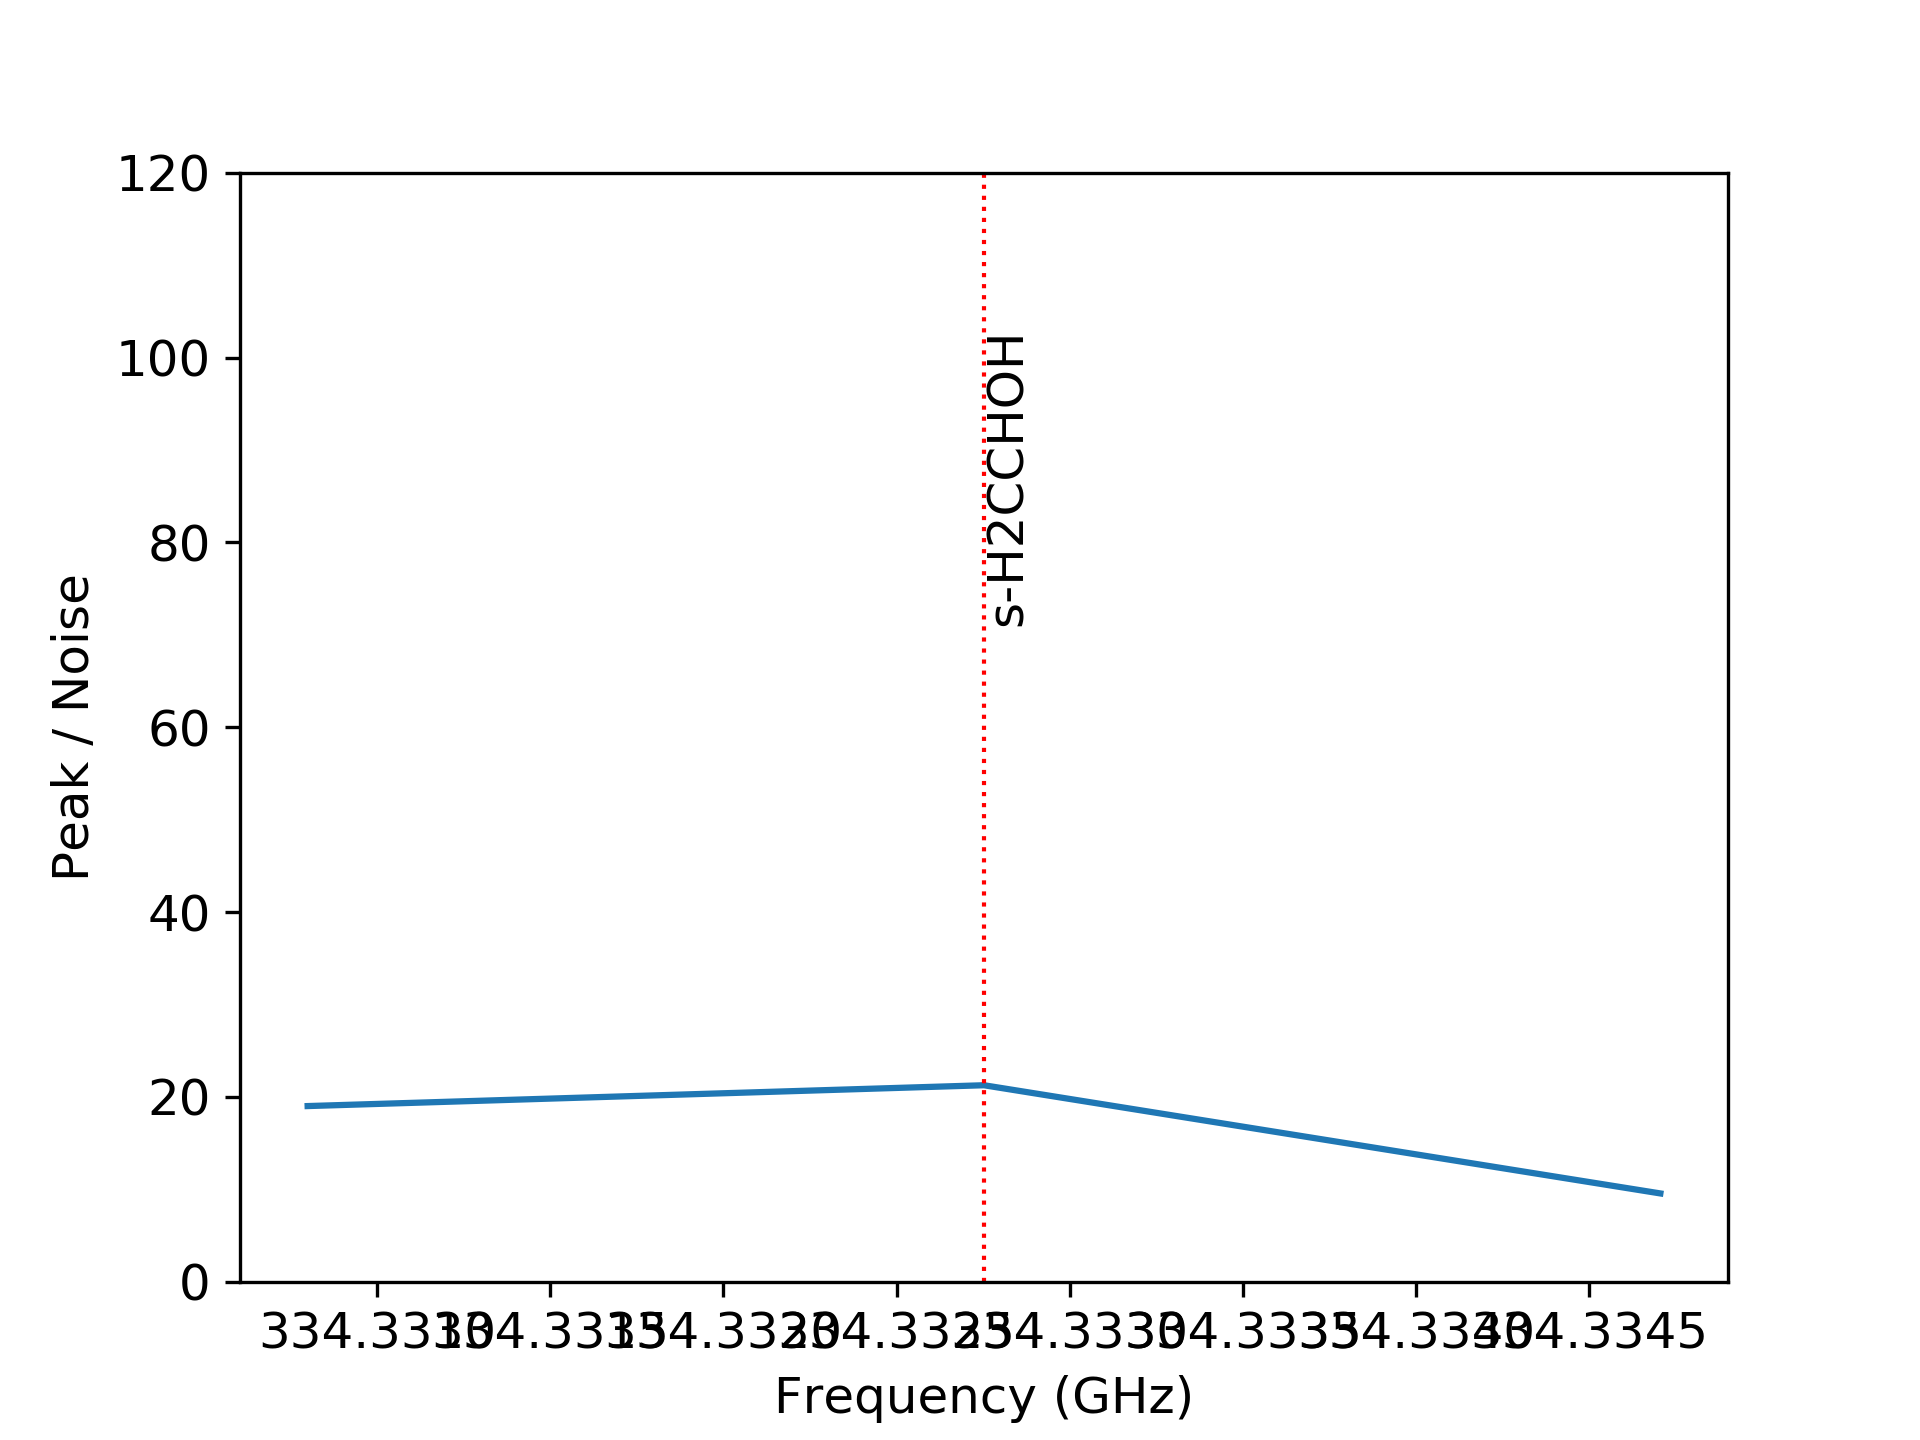
\includegraphics[width=0.33\textwidth]{spw2_s-H2CCHOH}

    \caption{Promising molecular lines identified in spectral window 2}
   \end{figure*}
   
      \begin{figure*}
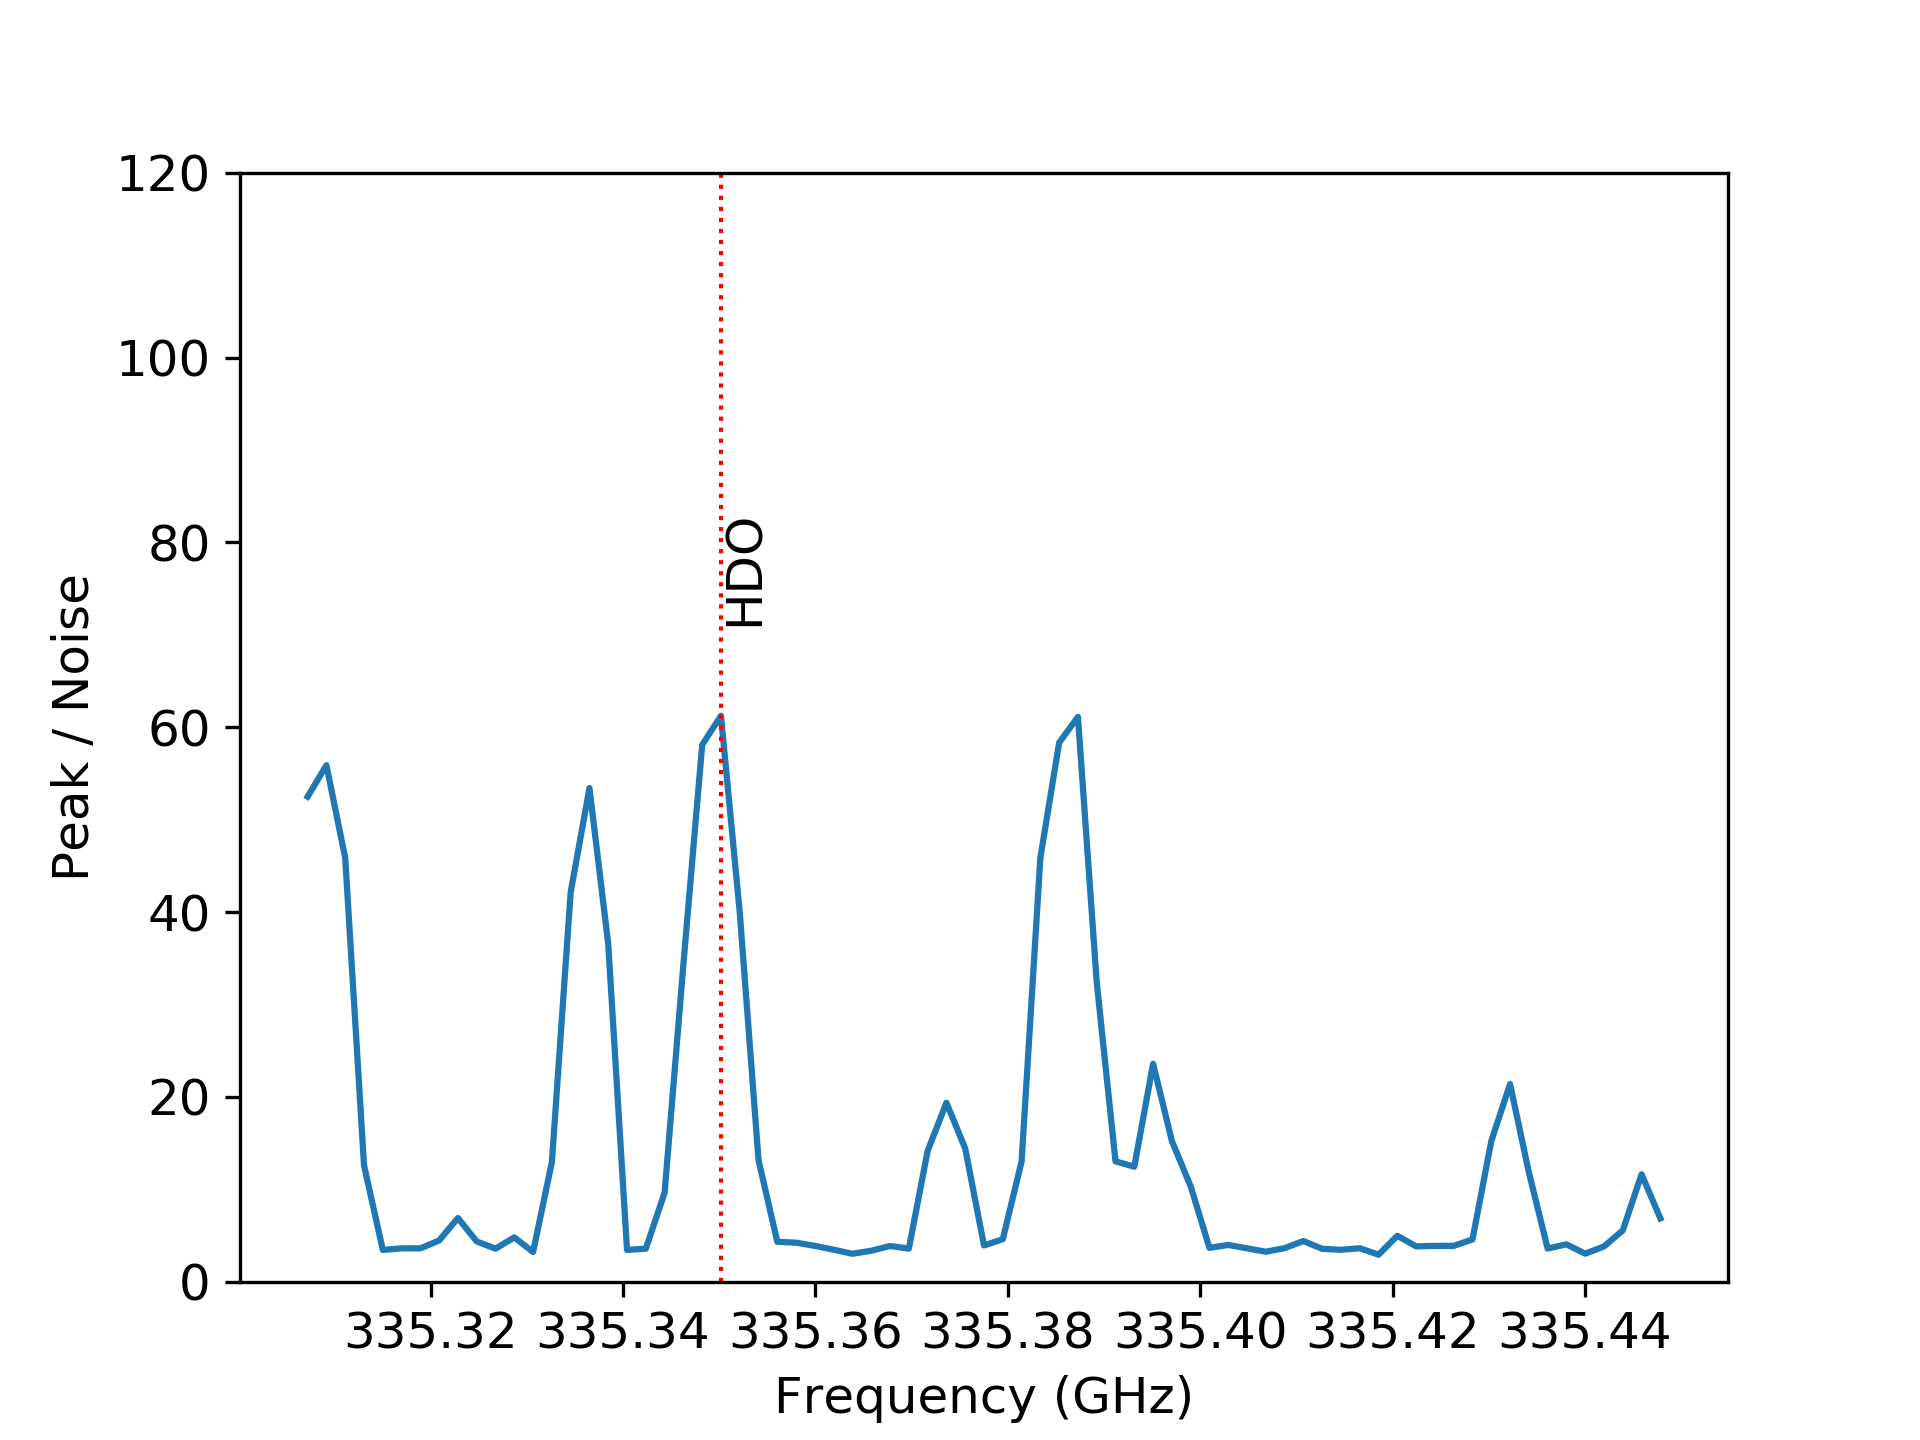
\includegraphics[width=0.33\textwidth]{spw2_HDO}
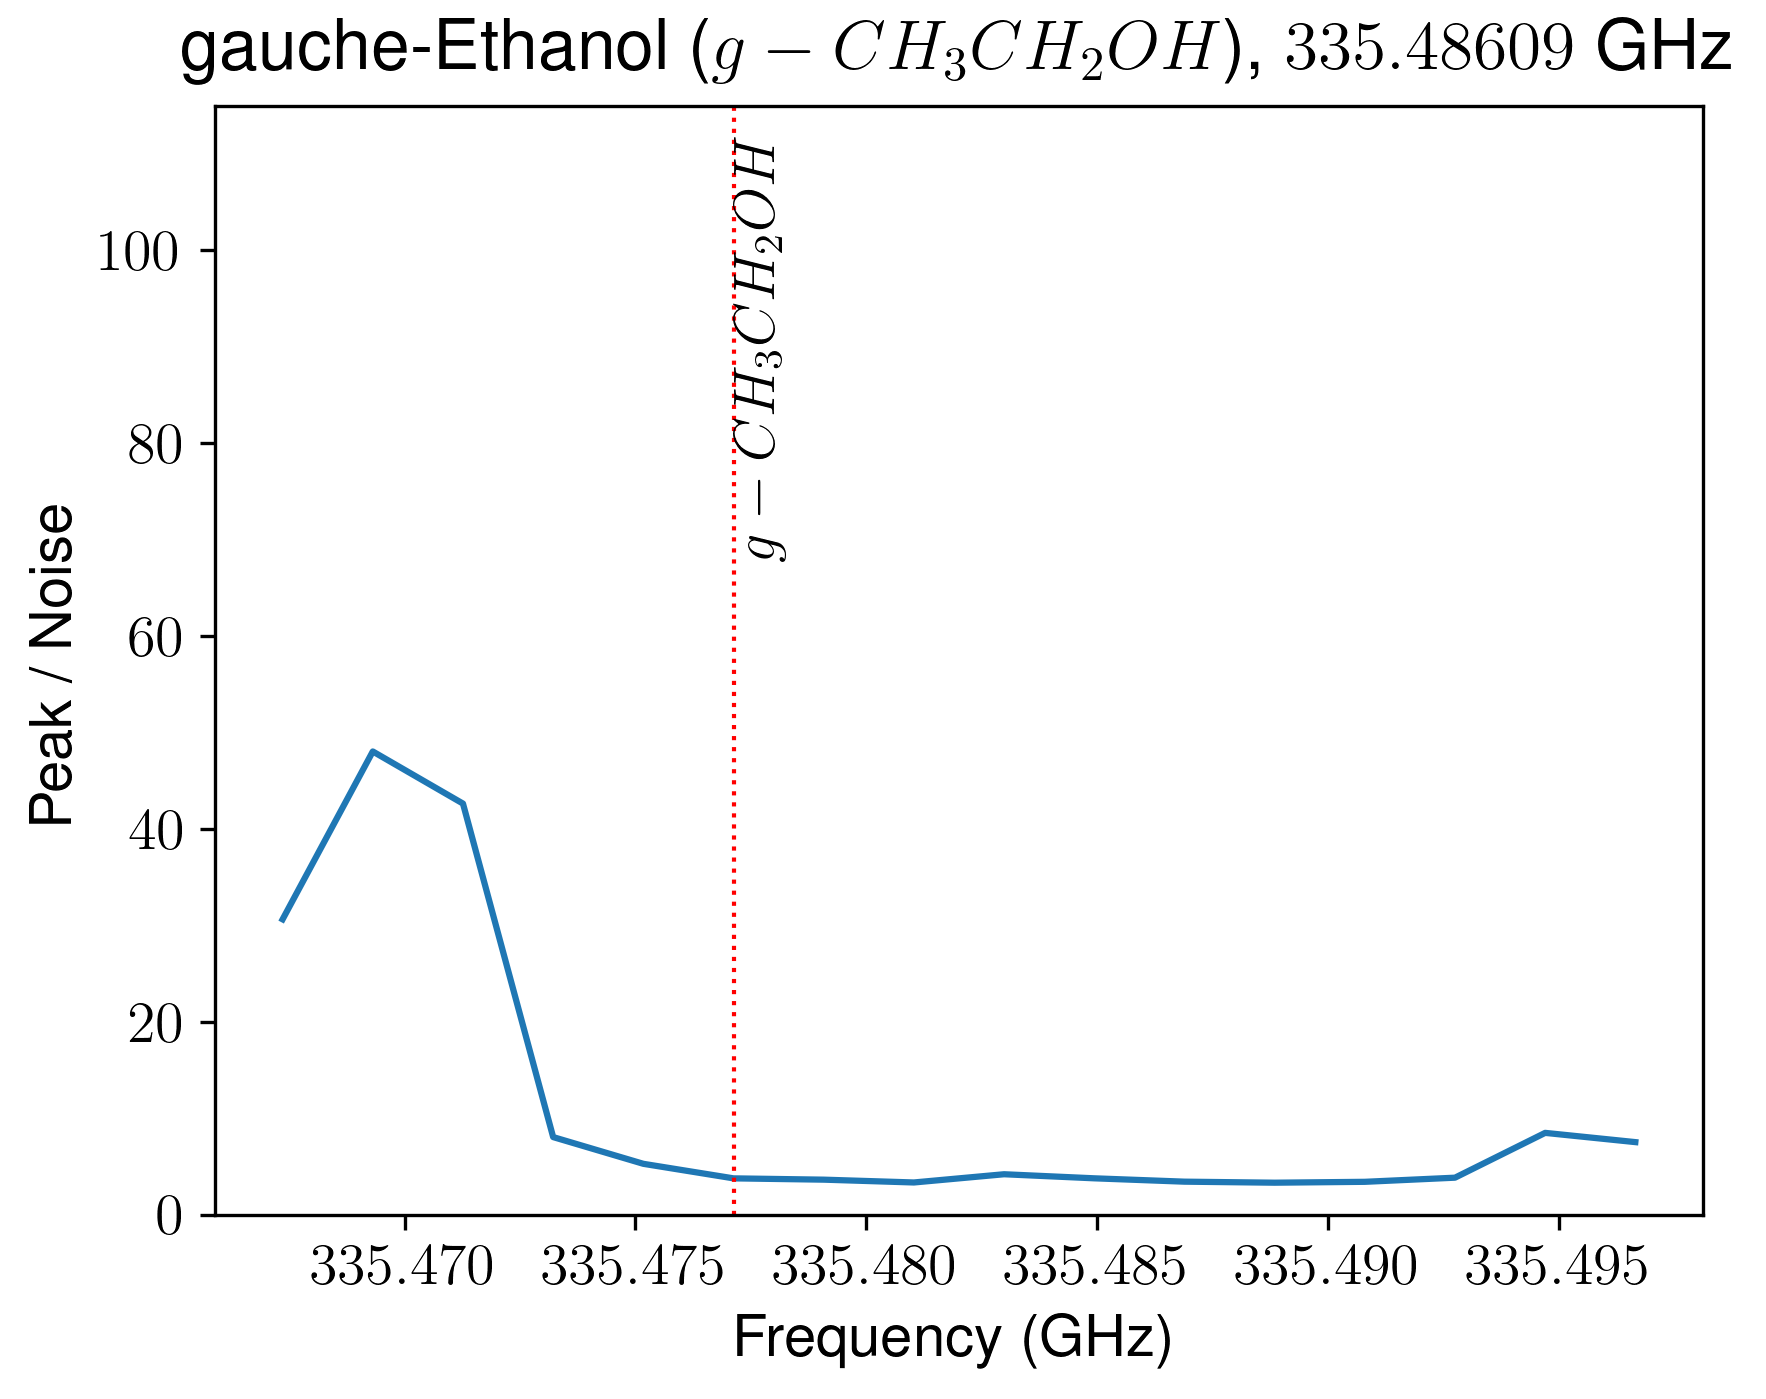
\includegraphics[width=0.33\textwidth]{spw2_g-CH3CH2OH}
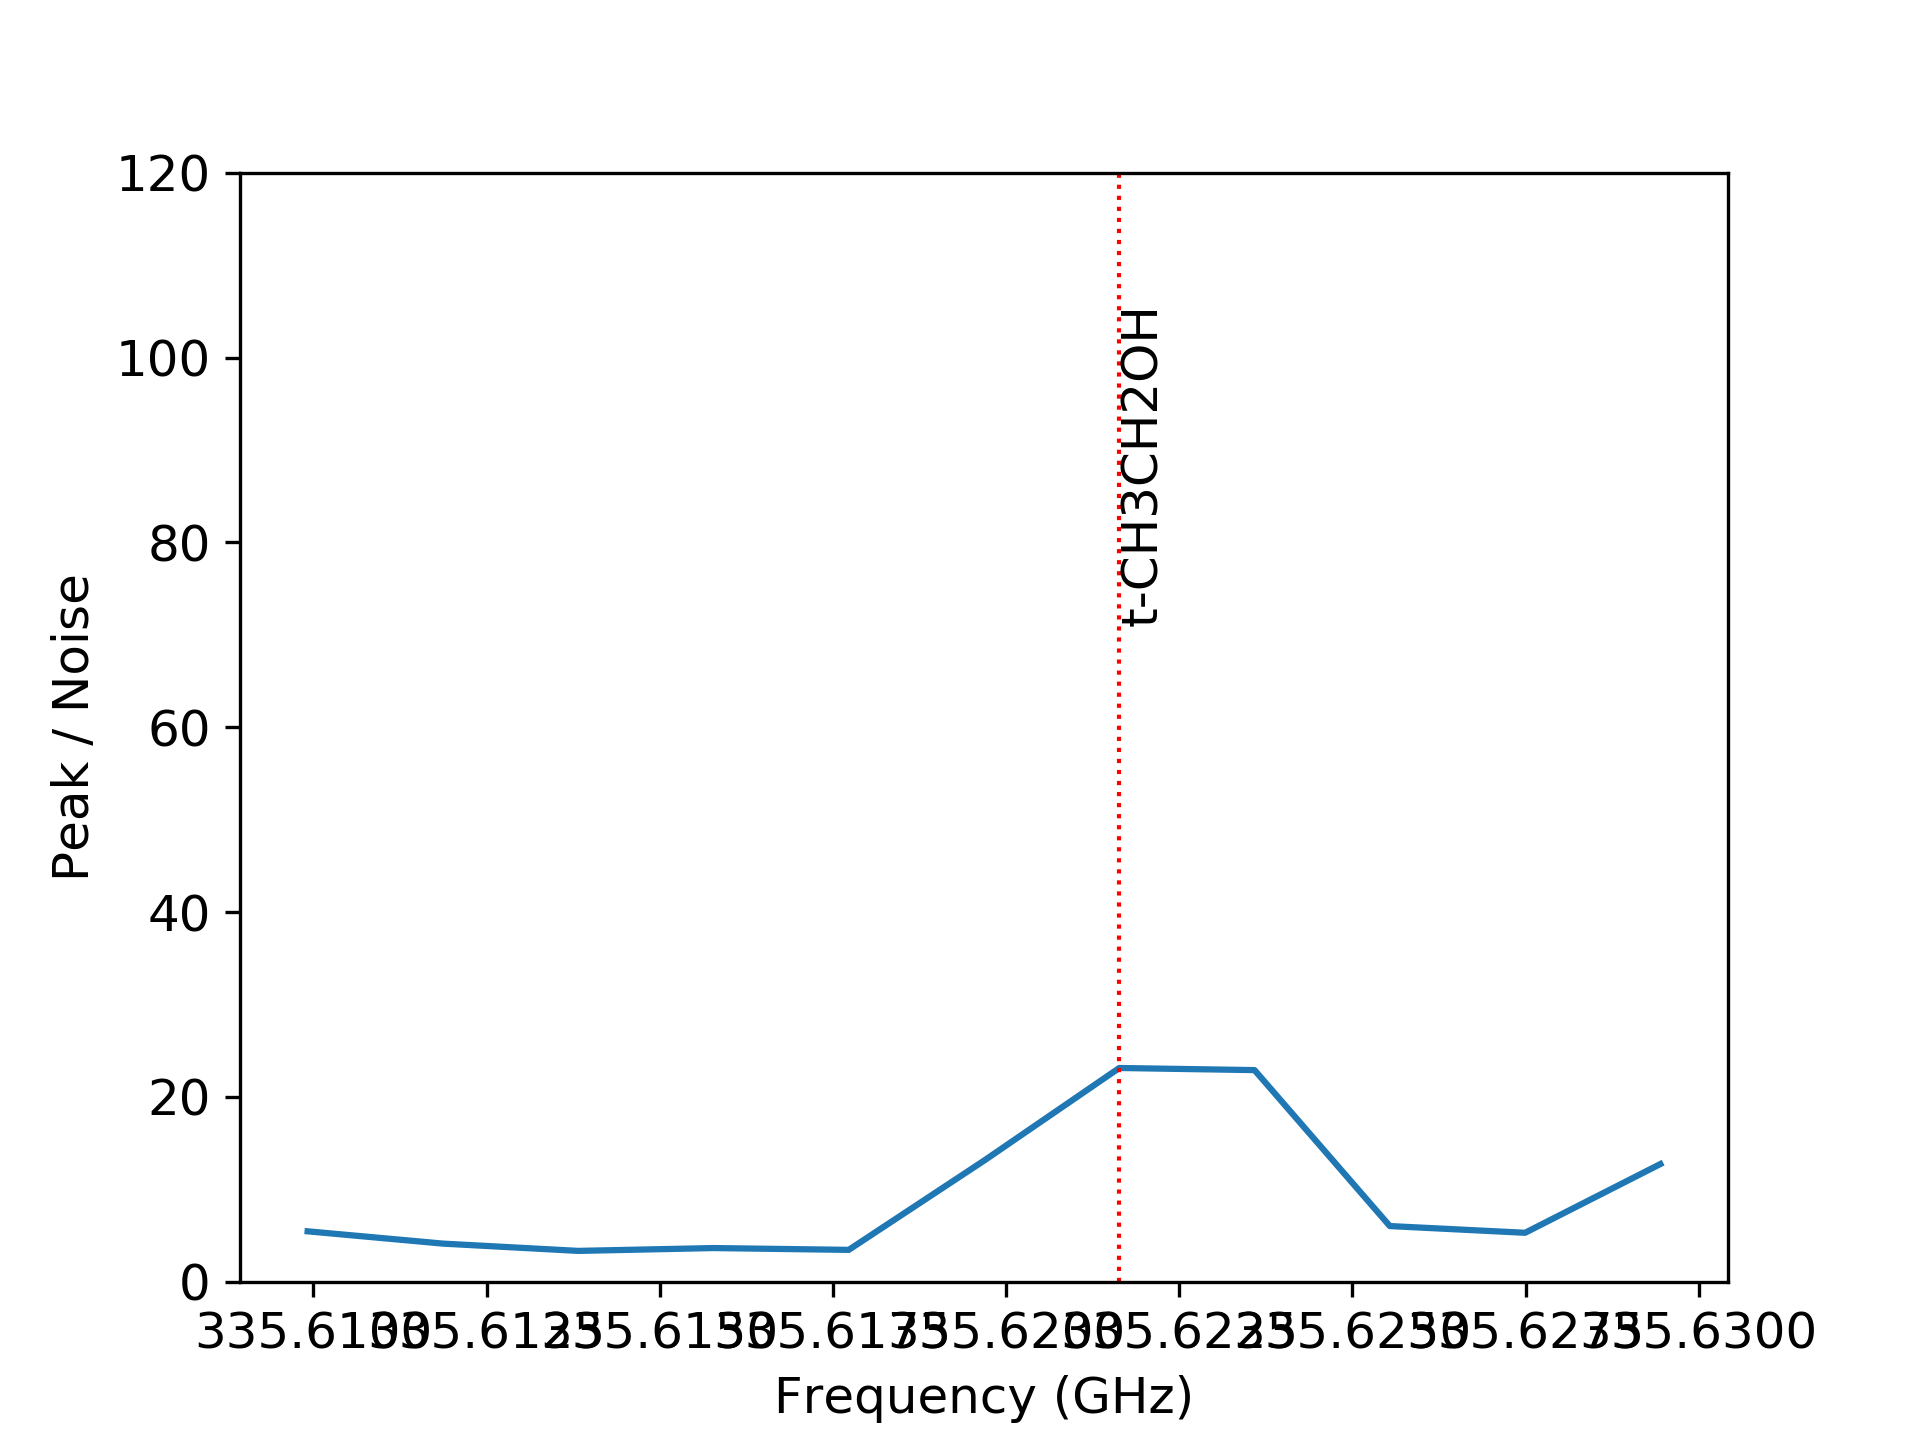
\includegraphics[width=0.33\textwidth]{spw2_t-CH3CH2OH}

    \caption{Promising molecular lines identified in spectral window 2 (continue)}
   \end{figure*}




\section{Conclusions}

   \begin{enumerate}
   \item Item placeholder
   \end{enumerate}


% WARNING
%-------------------------------------------------------------------
% Please note that we have included the references to the file aa.dem in
% order to compile it, but we ask you to:
%
% - use BibTeX with the regular commands:
%   \bibliographystyle{aa} % style aa.bst
%   \bibliography{Yourfile} % your references Yourfile.bib
%
% - join the .bib files when you upload your source files
%-------------------------------------------------------------------

\begin{thebibliography}{}

  \bibitem[Baker(1966)]{baker} Baker, N. 1966,
      in Stellar Evolution,
      ed.\ R. F. Stein,\& A. G. W. Cameron
      (Plenum, New York) 333
\end{thebibliography}

\end{document}
%
%%%%%%%%%%%%%%%%%%%%%%%%%%%%%%%%%%%%%%%%%%%%%%%%%%%%%%%%%%%%%%
Example below of non-structurated natbib references  
To use the v8.3 macros with this form of composition of bibliography, 
the option "bibyear" should be added to the command line 
"\documentclass[bibyear]{aa}".
%%%%%%%%%%%%%%%%%%%%%%%%%%%%%%%%%%%%%%%%%%%%%%%%%%%%%%%%%%%%%%

\begin{thebibliography}{}

  \bibitem[1966]{baker} Baker, N. 1966,
      in Stellar Evolution,
      ed.\ R. F. Stein,\& A. G. W. Cameron
      (Plenum, New York) 333

   \bibitem[1988]{balluch} Balluch, M. 1988,
      A\&A, 200, 58

   \bibitem[1980]{cox} Cox, J. P. 1980,
      Theory of Stellar Pulsation
      (Princeton University Press, Princeton) 16d5

   \bibitem[1969]{cox69} Cox, A. N.,\& Stewart, J. N. 1969,
      Academia Nauk, Scientific Information 15, 1

   \bibitem[1980]{mizuno} Mizuno H. 1980,
      Prog. Theor. Phys., 64, 544
   
   \bibitem[1987]{tscharnuter} Tscharnuter W. M. 1987,
      A\&A, 188, 55
  
   \bibitem[1992]{terlevich} Terlevich, R. 1992, in ASP Conf. Ser. 31, 
      Relationships between Active Galactic Nuclei and Starburst Galaxies, 
      ed. A. V. Filippenko, 13

   \bibitem[1980a]{yorke80a} Yorke, H. W. 1980a,
      A\&A, 86, 286

   \bibitem[1997]{zheng} Zheng, W., Davidsen, A. F., Tytler, D. \& Kriss, G. A.
      1997, preprint
\end{thebibliography}




















%-------------------------------------------------------------
%                 A figure as large as the width of the column
%-------------------------------------------------------------
   \begin{figure}
   \centering
   \includegraphics[width=\hsize]{empty.eps}
      \caption{Vibrational stability equation of state
               $S_{\mathrm{vib}}(\lg e, \lg \rho)$.
               $>0$ means vibrational stability.
              }
         \label{FigVibStab}
   \end{figure}
%
%-------------------------------------------------------------
%                                    One column rotated figure
%-------------------------------------------------------------
   \begin{figure}
   \centering
   \includegraphics[angle=-90,width=3cm]{empty.eps}
      \caption{Vibrational stability equation of state
               $S_{\mathrm{vib}}(\lg e, \lg \rho)$.
               $>0$ means vibrational stability.
              }
         \label{FigVibStab}
   \end{figure}
%
%-------------------------------------------------------------
%                        Figure with caption on the right side 
%-------------------------------------------------------------
   \begin{figure}
   \sidecaption
   \includegraphics[width=3cm]{empty.eps}
      \caption{Vibrational stability equation of state
               $S_{\mathrm{vib}}(\lg e, \lg \rho)$.
               $>0$ means vibrational stability.
              }
         \label{FigVibStab}
   \end{figure}
%
%-------------------------------------------------------------
%                                Figure with a new BoundingBox 
%-------------------------------------------------------------
   \begin{figure}
   \centering
   \includegraphics[bb=10 20 100 300,width=3cm,clip]{empty.eps}
      \caption{Vibrational stability equation of state
               $S_{\mathrm{vib}}(\lg e, \lg \rho)$.
               $>0$ means vibrational stability.
              }
         \label{FigVibStab}
   \end{figure}
%
%-------------------------------------------------------------
%                                      The "resizebox" command 
%-------------------------------------------------------------
   \begin{figure}
   \resizebox{\hsize}{!}
            {\includegraphics[bb=10 20 100 300,clip]{empty.eps}
      \caption{Vibrational stability equation of state
               $S_{\mathrm{vib}}(\lg e, \lg \rho)$.
               $>0$ means vibrational stability.
              }
         \label{FigVibStab}
   \end{figure}
%
%-------------------------------------------------------------
%                                             Two column Figure 
%-------------------------------------------------------------
   \begin{figure*}
   \resizebox{\hsize}{!}
            {\includegraphics[bb=10 20 100 300,clip]{empty.eps}
      \caption{Vibrational stability equation of state
               $S_{\mathrm{vib}}(\lg e, \lg \rho)$.
               $>0$ means vibrational stability.
              }
         \label{FigVibStab}
   \end{figure*}
%
%-------------------------------------------------------------
%                                             Simple A&A Table
%-------------------------------------------------------------
%
\begin{table}
\caption{Nonlinear Model Results}             % title of Table
\label{table:1}      % is used to refer this table in the text
\centering                          % used for centering table
\begin{tabular}{c c c c}        % centered columns (4 columns)
\hline\hline                 % inserts double horizontal lines
HJD & $E$ & Method\#2 & Method\#3 \\    % table heading 
\hline                        % inserts single horizontal line
   1 & 50 & $-837$ & 970 \\      % inserting body of the table
   2 & 47 & 877    & 230 \\
   3 & 31 & 25     & 415 \\
   4 & 35 & 144    & 2356 \\
   5 & 45 & 300    & 556 \\ 
\hline                                   %inserts single line
\end{tabular}
\end{table}

%
%-------------------------------------------------------------
%                                          Table with notes 
%-------------------------------------------------------------
%
% A single note
\begin{table}
\caption{\label{t7}Spectral types and photometry for stars in the
  region.}
\centering
\begin{tabular}{lccc}
\hline\hline
Star&Spectral type&RA(J2000)&Dec(J2000)\\
\hline
69           &B1\,V     &09 15 54.046 & $-$50 00 26.67\\
49           &B0.7\,V   &*09 15 54.570& $-$50 00 03.90\\
LS~1267~(86) &O8\,V     &09 15 52.787&11.07\\
24.6         &7.58      &1.37 &0.20\\
\hline
LS~1262      &B0\,V     &09 15 05.17&11.17\\
MO 2-119     &B0.5\,V   &09 15 33.7 &11.74\\
LS~1269      &O8.5\,V   &09 15 56.60&10.85\\
\hline
\end{tabular}
\tablefoot{The top panel shows likely members of Pismis~11. The second
panel contains likely members of Alicante~5. The bottom panel
displays stars outside the clusters.}
\end{table}
%
% More notes
%
\begin{table}
\caption{\label{t7}Spectral types and photometry for stars in the
  region.}
\centering
\begin{tabular}{lccc}
\hline\hline
Star&Spectral type&RA(J2000)&Dec(J2000)\\
\hline
69           &B1\,V     &09 15 54.046 & $-$50 00 26.67\\
49           &B0.7\,V   &*09 15 54.570& $-$50 00 03.90\\
LS~1267~(86) &O8\,V     &09 15 52.787&11.07\tablefootmark{a}\\
24.6         &7.58\tablefootmark{1}&1.37\tablefootmark{a}   &0.20\tablefootmark{a}\\
\hline
LS~1262      &B0\,V     &09 15 05.17&11.17\tablefootmark{b}\\
MO 2-119     &B0.5\,V   &09 15 33.7 &11.74\tablefootmark{c}\\
LS~1269      &O8.5\,V   &09 15 56.60&10.85\tablefootmark{d}\\
\hline
\end{tabular}
\tablefoot{The top panel shows likely members of Pismis~11. The second
panel contains likely members of Alicante~5. The bottom panel
displays stars outside the clusters.\\
\tablefoottext{a}{Photometry for MF13, LS~1267 and HD~80077 from
Dupont et al.}
\tablefoottext{b}{Photometry for LS~1262, LS~1269 from
Durand et al.}
\tablefoottext{c}{Photometry for MO2-119 from
Mathieu et al.}
}
\end{table}
%
%-------------------------------------------------------------
%                                       Table with references 
%-------------------------------------------------------------
%
\begin{table*}[h]
 \caption[]{\label{nearbylistaa2}List of nearby SNe used in this work.}
\begin{tabular}{lccc}
 \hline \hline
  SN name &
  Epoch &
 Bands &
  References \\
 &
  (with respect to $B$ maximum) &
 &
 \\ \hline
1981B   & 0 & {\it UBV} & 1\\
1986G   &  $-$3, $-$1, 0, 1, 2 & {\it BV}  & 2\\
1989B   & $-$5, $-$1, 0, 3, 5 & {\it UBVRI}  & 3, 4\\
1990N   & 2, 7 & {\it UBVRI}  & 5\\
1991M   & 3 & {\it VRI}  & 6\\
\hline
\noalign{\smallskip}
\multicolumn{4}{c}{ SNe 91bg-like} \\
\noalign{\smallskip}
\hline
1991bg   & 1, 2 & {\it BVRI}  & 7\\
1999by   & $-$5, $-$4, $-$3, 3, 4, 5 & {\it UBVRI}  & 8\\
\hline
\noalign{\smallskip}
\multicolumn{4}{c}{ SNe 91T-like} \\
\noalign{\smallskip}
\hline
1991T   & $-$3, 0 & {\it UBVRI}  &  9, 10\\
2000cx  & $-$3, $-$2, 0, 1, 5 & {\it UBVRI}  & 11\\ %
\hline
\end{tabular}
\tablebib{(1)~\citet{branch83};
(2) \citet{phillips87}; (3) \citet{barbon90}; (4) \citet{wells94};
(5) \citet{mazzali93}; (6) \citet{gomez98}; (7) \citet{kirshner93};
(8) \citet{patat96}; (9) \citet{salvo01}; (10) \citet{branch03};
(11) \citet{jha99}.
}
\end{table}
%-------------------------------------------------------------
%                      A rotated Two column Table in landscape  
%-------------------------------------------------------------
\begin{sidewaystable*}
\caption{Summary for ISOCAM sources with mid-IR excess 
(YSO candidates).}\label{YSOtable}
\centering
\begin{tabular}{crrlcl} 
\hline\hline             
ISO-L1551 & $F_{6.7}$~[mJy] & $\alpha_{6.7-14.3}$ 
& YSO type$^{d}$ & Status & Comments\\
\hline
  \multicolumn{6}{c}{\it New YSO candidates}\\ % To combine 6 columns into a single one
\hline
  1 & 1.56 $\pm$ 0.47 & --    & Class II$^{c}$ & New & Mid\\
  2 & 0.79:           & 0.97: & Class II ?     & New & \\
  3 & 4.95 $\pm$ 0.68 & 3.18  & Class II / III & New & \\
  5 & 1.44 $\pm$ 0.33 & 1.88  & Class II       & New & \\
\hline
  \multicolumn{6}{c}{\it Previously known YSOs} \\
\hline
  61 & 0.89 $\pm$ 0.58 & 1.77 & Class I & \object{HH 30} & Circumstellar disk\\
  96 & 38.34 $\pm$ 0.71 & 37.5& Class II& MHO 5          & Spectral type\\
\hline
\end{tabular}
\end{sidewaystable*}
%-------------------------------------------------------------
%                      A rotated One column Table in landscape  
%-------------------------------------------------------------
\begin{sidewaystable}
\caption{Summary for ISOCAM sources with mid-IR excess 
(YSO candidates).}\label{YSOtable}
\centering
\begin{tabular}{crrlcl} 
\hline\hline             
ISO-L1551 & $F_{6.7}$~[mJy] & $\alpha_{6.7-14.3}$ 
& YSO type$^{d}$ & Status & Comments\\
\hline
  \multicolumn{6}{c}{\it New YSO candidates}\\ % To combine 6 columns into a single one
\hline
  1 & 1.56 $\pm$ 0.47 & --    & Class II$^{c}$ & New & Mid\\
  2 & 0.79:           & 0.97: & Class II ?     & New & \\
  3 & 4.95 $\pm$ 0.68 & 3.18  & Class II / III & New & \\
  5 & 1.44 $\pm$ 0.33 & 1.88  & Class II       & New & \\
\hline
  \multicolumn{6}{c}{\it Previously known YSOs} \\
\hline
  61 & 0.89 $\pm$ 0.58 & 1.77 & Class I & \object{HH 30} & Circumstellar disk\\
  96 & 38.34 $\pm$ 0.71 & 37.5& Class II& MHO 5          & Spectral type\\
\hline
\end{tabular}
\end{sidewaystable}
%
%-------------------------------------------------------------
%                              Table longer than a single page  
%-------------------------------------------------------------
% All long tables will be placed automatically at the end of the document
%
\longtab{
\begin{longtable}{lllrrr}
\caption{\label{kstars} Sample stars with absolute magnitude}\\
\hline\hline
Catalogue& $M_{V}$ & Spectral & Distance & Mode & Count Rate \\
\hline
\endfirsthead
\caption{continued.}\\
\hline\hline
Catalogue& $M_{V}$ & Spectral & Distance & Mode & Count Rate \\
\hline
\endhead
\hline
\endfoot
%%
Gl 33    & 6.37 & K2 V & 7.46 & S & 0.043170\\
Gl 66AB  & 6.26 & K2 V & 8.15 & S & 0.260478\\
Gl 68    & 5.87 & K1 V & 7.47 & P & 0.026610\\
         &      &      &      & H & 0.008686\\
Gl 86 
\footnote{Source not included in the HRI catalog. See Sect.~5.4.2 for details.}
         & 5.92 & K0 V & 10.91& S & 0.058230\\
\end{longtable}
}
%
%-------------------------------------------------------------
%                              Table longer than a single page
%                                            and in landscape, 
%                    in the preamble, use: \usepackage{lscape}
%-------------------------------------------------------------

% All long tables will be placed automatically at the end of the document
%
\longtab{
\begin{landscape}
\begin{longtable}{lllrrr}
\caption{\label{kstars} Sample stars with absolute magnitude}\\
\hline\hline
Catalogue& $M_{V}$ & Spectral & Distance & Mode & Count Rate \\
\hline
\endfirsthead
\caption{continued.}\\
\hline\hline
Catalogue& $M_{V}$ & Spectral & Distance & Mode & Count Rate \\
\hline
\endhead
\hline
\endfoot
%%
Gl 33    & 6.37 & K2 V & 7.46 & S & 0.043170\\
Gl 66AB  & 6.26 & K2 V & 8.15 & S & 0.260478\\
Gl 68    & 5.87 & K1 V & 7.47 & P & 0.026610\\
         &      &      &      & H & 0.008686\\
Gl 86
\footnote{Source not included in the HRI catalog. See Sect.~5.4.2 for details.}
         & 5.92 & K0 V & 10.91& S & 0.058230\\
\end{longtable}
\end{landscape}
}
%
%-------------------------------------------------------------
%               Appendices have to be placed at the end, after
%                                        \end{thebibliography}
%-------------------------------------------------------------
\end{thebibliography}

\begin{appendix} %First appendix
\section{Background galaxy number counts and shear noise-levels}
Because the optical images used in this analysis...
\begin{figure*}%f1
\includegraphics[width=10.9cm]{1787f23.eps}
\caption{Shown in greyscale is a...}
\label{cl12301}
\end{figure*}

In this case....
\begin{figure*}
\centering
\includegraphics[width=16.4cm,clip]{1787f24.ps}
\caption{Plotted above...}
\label{appfig}
\end{figure*}

Because the optical images...

\section{Title of Second appendix.....} %Second appendix
These studies, however, have faced...
\begin{table}
\caption{Complexes characterisation.}\label{starbursts}
\centering
\begin{tabular}{lccc}
\hline \hline
Complex & $F_{60}$ & 8.6 &  No. of  \\
...
\hline
\end{tabular}
\end{table}

The second method produces...
\end{appendix}
%
%
\end{document}

%
%-------------------------------------------------------------
%          For the appendices, table longer than a single page
%-------------------------------------------------------------

% Table will be print automatically at the end of the document, 
% after the whole appendices

\begin{appendix} %First appendix
\section{Background galaxy number counts and shear noise-levels}

% In the appendices do not forget to put the counter of the table 
% as an option

\longtab[1]{
\begin{longtable}{lrcrrrrrrrrl}
\caption{Line data and abundances ...}\\
\hline
\hline
Def & mol & Ion & $\lambda$ & $\chi$ & $\log gf$ & N & e &  rad & $\delta$ & $\delta$ 
red & References \\
\hline
\endfirsthead
\caption{Continued.} \\
\hline
Def & mol & Ion & $\lambda$ & $\chi$ & $\log gf$ & B & C &  rad & $\delta$ & $\delta$ 
red & References \\
\hline
\endhead
\hline
\endfoot
\hline
\endlastfoot
A & CH & 1 &3638 & 0.002 & $-$2.551 &  &  &  & $-$150 & 150 &  Jorgensen et al. (1996) \\                    
\end{longtable}
}% End longtab
\end{appendix}

%-------------------------------------------------------------
%                   For appendices and landscape, large table:
%                    in the preamble, use: \usepackage{lscape}
%-------------------------------------------------------------

\begin{appendix} %First appendix
%
\longtab[1]{
\begin{landscape}
\begin{longtable}{lrcrrrrrrrrl}
...
\end{longtable}
\end{landscape}
}% End longtab
\end{appendix}

%%%% End of aa.dem
